\documentclass[10pt,a4paper]{article}
\usepackage{blindtext}
\usepackage{subcaption}
\usepackage{graphicx}
\usepackage{tikz}
\usepackage{amssymb}
\usepackage{caption}
\usepackage{amsmath}
\usepackage{circuitikz}
\usepackage{hyperref}
\usepackage{amssymb}
\usepackage{amsmath}
\usepackage{listings}
\usepackage{comment} 
\renewcommand{\familydefault}{\sfdefault}
\lstset{columns=fullflexible,basicstyle=\ttfamily}
\usepackage[top=1cm,bottom=2cm,left=1cm,right=1cm]{geometry}%

\lstset{
    inputencoding=utf8,
    extendedchars=true,
    literate={á}{{\'a}}1 {é}{{\'e}}1 {í}{{\'i}}1 {ó}{{\'o}}1 {ú}{{\'u}}1 {ñ}{{\~n}}1 {Á}{{\'A}}1 {É}{{\'E}}1 {Í}{{\'I}}1 {Ó}{{\'O}}1 {Ú}{{\'U}}1 {Ñ}{{\~N}}1
}
\usepackage[spanish,activeacute,es-tabla]{babel}
\usepackage[utf8]{inputenc}
\usepackage{ifthen}
\usepackage{listings}
\usepackage{dsfont}
\usepackage{subcaption}
\usepackage{amsmath}
\usepackage[strict]{changepage}
\usepackage[top=1cm,bottom=2cm,left=1cm,right=1cm]{geometry}%
\usepackage{color}%
\newcommand{\tocarEspacios}{%
	\addtolength{\leftskip}{3em}%
	\setlength{\parindent}{0em}%
}

% Especificacion de procs

\newcommand{\In}{\textsf{in }}
\newcommand{\Out}{\textsf{out }}
\newcommand{\Inout}{\textsf{inout }}

\newcommand{\encabezadoDeProc}[4]{%
	% Ponemos la palabrita problema en tt
	%  \noindent%
	{\normalfont\bfseries\ttfamily proc}%
	% Ponemos el nombre del problema
	\ %
	{\normalfont\ttfamily #2}%
	\
	% Ponemos los parametros
	(#3)%
	\ifthenelse{\equal{#4}{}}{}{%
		% Por ultimo, va el tipo del resultado
		\ : #4}
}

\newenvironment{proc}[4][res]{%
	
	% El parametro 1 (opcional) es el nombre del resultado
	% El parametro 2 es el nombre del problema
	% El parametro 3 son los parametros
	% El parametro 4 es el tipo del resultado
	% Preambulo del ambiente problema
	% Tenemos que definir los comandos requiere, asegura, modifica y aux
	\newcommand{\requiere}[2][]{%
		{\normalfont\bfseries\ttfamily requiere}%
		\ifthenelse{\equal{##1}{}}{}{\ {\normalfont\ttfamily ##1} :}\ %
		\{\ensuremath{##2}\}%
		{\normalfont\bfseries\,\par}%
	}
	\newcommand{\asegura}[2][]{%
		{\normalfont\bfseries\ttfamily asegura}%
		\ifthenelse{\equal{##1}{}}{}{\ {\normalfont\ttfamily ##1} :}\
		\{\ensuremath{##2}\}%
		{\normalfont\bfseries\,\par}%
	}
	\renewcommand{\aux}[4]{%
		{\normalfont\bfseries\ttfamily aux\ }%
		{\normalfont\ttfamily ##1}%
		\ifthenelse{\equal{##2}{}}{}{\ (##2)}\ : ##3\, = \ensuremath{##4}%
		{\normalfont\bfseries\,;\par}%
	}
	\renewcommand{\pred}[3]{%
		{\normalfont\bfseries\ttfamily pred }%
		{\normalfont\ttfamily ##1}%
		\ifthenelse{\equal{##2}{}}{}{\ (##2) }%
		\{%
		\begin{adjustwidth}{+5em}{}
			\ensuremath{##3}
		\end{adjustwidth}
		\}%
		{\normalfont\bfseries\,\par}%
	}
	
	\newcommand{\res}{#1}
	\vspace{1ex}
	\noindent
	\encabezadoDeProc{#1}{#2}{#3}{#4}
	% Abrimos la llave
	\par%
	\tocarEspacios
}
{
	% Cerramos la llave
	\vspace{1ex}
}

\newcommand{\aux}[4]{%
	{\normalfont\bfseries\ttfamily\noindent aux\ }%
	{\normalfont\ttfamily #1}%
	\ifthenelse{\equal{#2}{}}{}{\ (#2)}\ : #3\, = \ensuremath{#4}%
	{\normalfont\bfseries\,;\par}%
}

\newcommand{\pred}[3]{%
	{\normalfont\bfseries\ttfamily\noindent pred }%
	{\normalfont\ttfamily #1}%
	\ifthenelse{\equal{#2}{}}{}{\ (#2) }%
	\{%
	\begin{adjustwidth}{+2em}{}
		\ensuremath{#3}
	\end{adjustwidth}
	\}%
	{\normalfont\bfseries\,\par}%
}

% Tipos

\newcommand{\nat}{\ensuremath{\mathds{N}}}
\newcommand{\ent}{\ensuremath{\mathds{Z}}}
\newcommand{\float}{\ensuremath{\mathds{R}}}
\newcommand{\bool}{\ensuremath{\mathsf{Bool}}}
\newcommand{\cha}{\ensuremath{\mathsf{Char}}}
\newcommand{\str}{\ensuremath{\mathsf{String}}}

% Logica

\newcommand{\True}{\ensuremath{\mathrm{true}}}
\newcommand{\False}{\ensuremath{\mathrm{false}}}
\newcommand{\Then}{\ensuremath{\rightarrow}}
\newcommand{\Iff}{\ensuremath{\leftrightarrow}}
\newcommand{\implica}{\ensuremath{\longrightarrow}}
\newcommand{\IfThenElse}[3]{\ensuremath{\mathsf{if}\ #1\ \mathsf{then}\ #2\ \mathsf{else}\ #3\ \mathsf{fi}}}
\newcommand{\yLuego}{\land _L}
\newcommand{\oLuego}{\lor _L}
\newcommand{\implicaLuego}{\implica _L}

\newcommand{\cuantificador}[5]{%
	\ensuremath{(#2 #3: #4)\ (%
		\ifthenelse{\equal{#1}{unalinea}}{
			#5
		}{
			$ % exiting math mode
			\begin{adjustwidth}{+2em}{}
				$#5$%
			\end{adjustwidth}%
			$ % entering math mode
		}
		)}
}

\newcommand{\existe}[4][]{%
	\cuantificador{#1}{\exists}{#2}{#3}{#4}
}
\newcommand{\paraTodo}[4][]{%
	\cuantificador{#1}{\forall}{#2}{#3}{#4}
}

%listas

\newcommand{\TLista}[1]{\ensuremath{seq \langle #1\rangle}}
\newcommand{\lvacia}{\ensuremath{[\ ]}}
\newcommand{\lv}{\ensuremath{[\ ]}}
\newcommand{\longitud}[1]{\ensuremath{|#1|}}
\newcommand{\cons}[1]{\ensuremath{\mathsf{addFirst}}(#1)}
\newcommand{\indice}[1]{\ensuremath{\mathsf{indice}}(#1)}
\newcommand{\conc}[1]{\ensuremath{\mathsf{concat}}(#1)}
\newcommand{\cab}[1]{\ensuremath{\mathsf{head}}(#1)}
\newcommand{\cola}[1]{\ensuremath{\mathsf{tail}}(#1)}
\newcommand{\sub}[1]{\ensuremath{\mathsf{subseq}}(#1)}
\newcommand{\en}[1]{\ensuremath{\mathsf{en}}(#1)}
\newcommand{\cuenta}[2]{\mathsf{cuenta}\ensuremath{(#1, #2)}}
\newcommand{\suma}[1]{\mathsf{suma}(#1)}
\newcommand{\twodots}{\ensuremath{\mathrm{..}}}
\newcommand{\masmas}{\ensuremath{++}}
\newcommand{\matriz}[1]{\TLista{\TLista{#1}}}
\newcommand{\seqchar}{\TLista{\cha}}

\renewcommand{\lstlistingname}{Código}
\lstset{% general command to set parameter(s)
	language=Java,
	morekeywords={endif, endwhile, skip},
	basewidth={0.47em,0.40em},
	columns=fixed, fontadjust, resetmargins, xrightmargin=5pt, xleftmargin=15pt,
	flexiblecolumns=false, tabsize=4, breaklines, breakatwhitespace=false, extendedchars=true,
	numbers=left, numberstyle=\tiny, stepnumber=1, numbersep=9pt,
	frame=l, framesep=3pt,
	captionpos=b,
}

\newcommand{\barratexto}[3]{
    \begin{tikzpicture}
        \draw[thick] (0,0) -- (3,0);
        \node at (1.5, 0.3) {#1};
        \node at (1.5,-0.5) {#2}; 
        \node at (4,0) {#3}; 
    \end{tikzpicture}
}
\newcommand{\sd}[3]{
    \begin{tikzpicture}
        % Nodos para las expresiones matemáticas
        \node (A) at (0,0) {\(#1\)};
        \node (B) at (0,-1) {\(#2\)};
        
        % Dibujar la línea horizontal en el medio
        \draw[thick] (-2, -0.5) -- (2, -0.5);  
        
        % Colocar el texto del tercer parámetro al final de la línea
        \node[anchor=west] at (2.2, -0.5) {#3};
    \end{tikzpicture}
}

\newcommand{\equivDef}[1]{%
  \underset{#1}{\equiv}%
}



\newcommand{\notimplies}{\;\not\!\!\!\implies}
\title{Paradigmas de Lenguajes de Programación}
\author{Tomás Agustín Hernández}
\date{}

\begin{document}
\maketitle

\begin{figure}[b]
    \centering
    \begin{tikzpicture}[remember picture,overlay]
        \node[anchor=south east, inner sep=0pt, xshift=-1cm, yshift=2cm] at (current page.south east) {
            \begin{minipage}[b]{0.5\textwidth}
                
\includegraphics[width=\linewidth]{logo_uba.jpg}
                \label{fig:bottom}
            \end{minipage}
        };
    \end{tikzpicture}
\end{figure}

\newpage
\section*{Programación Funcional}
Consiste en definir funciones y aplicarlas para procesar información. \\
Las funciones son verdaderamente funciones (parciales): 
\begin{itemize}
    \item Aplicar una función no tiene efectos secundarios.
    \item A una misma entrada le corresponde siempre la misma salida.
    \item Las estructuras de datos son inmutables.
\end{itemize}
Las funciones, además son datos como cualquier otro:
\begin{itemize}
    \item Se pueden pasar como parámetros.
    \item Se pueden devolver como resultados.
    \item Pueden formar parte de estructuras de datos. Ej.: Un árbol binario que en sus nodos hay funciones.
\end{itemize}
\subsection*{Expresiones}
Son secuencias de símbolos que sirven para representar datos, funciones, y funciones aplicadas a los datos. \\
Una expresión puede ser:
\begin{itemize}
    \item Un constructor: True, False, [], (:), 0, 1, 2. 
    \begin{itemize}
        \item Type Constructor: Es un constructor que se utiliza para crear un nuevo tipo.
        \item Data Constructor: Se utiliza para crear valores de ese tipo.
        \item Ej.: $data \ Color \ = \ Rojo \ | \ Verde \ | \ Azul$. Azul es un \textbf{data constructor} pues nos permite crear valores del tipo Color mientras que el Type Constructor es Color.
        \item Ej.: $data \ Complejo \ = \ C \ Float \ Float $. C es una función que recibe dos Float y es un constructor de Complejo.
    \end{itemize}
    \item Una variable: longitud, ordenar, x, xs (+), (*). 
    \item La aplicación de una expresión a otra: ordenar lista, not True, (+) 1. 
\end{itemize}
\subsection*{Función Parcialmente Aplicada}
Una función parcialmente aplicada es una función a las cuales se llama otra función pero no se le proporcionan todos los argumentos. \\
Ahora, es importante que para que esta función parcialmente aplicada tenga sentido se le manden todos los parámetros. \\
Es una especie de $ a \rightarrow b$
Ej.: 
\begin{lstlisting}
    add :: Int -> Int -> Int
    add x y = x + y

    add5 :: Int -> Int
    add5 = add 5

    add5 es una función que ejecuta la función parcial add pues le manda solo un parámetro y necesita dos.
   
\end{lstlisting}
Una buena pregunta entonces es ¿pero por qué es una función parcial add 5? Pues hay una función add5 que la implementa sin pasarle todos los parámetros directamente explícitamente.
\begin{lstlisting}
    add5 3 -> Este 3 llega como "y" a add

    add5 = add 5 
    add = 5 + y
    add = 5 + 3
    add = 8 

\end{lstlisting}

Otro ejemplo 
\begin{lstlisting}
    const :: a -> b -> a 
    const x y = x

    const (const 1) 2 -> const 1
    El llamado de (const 1) es una función parcialmente aplicada porque no envía el valor de y, sin embargo, const (const 1) 2 no la aplica parcialmente porque le termina mandando los dos parámetros.
\end{lstlisting}

\subsection*{Aplicación de Expresiones}
Es asociativa hacia la izquierda:
\begin{itemize}
    \item $ f \ x \ y \equiv \ (f \ x) \ y $
    \item $ ((((f \ a) \ b) \ c) \ d)$: Primero calcula el resultado que devuelve la expresión f enviando el valor de a. Nótese que la ídea seria que (f a) devuelva una expresión del tipo función pues luego le pasamos otro parámetro (b).
\end{itemize}
\subsection*{Importancia de la Aplicación de las Expresiones}
¿Qué sucede si aplicamos Head Tail l? Recordemos que la asociatividad a la izquierda haría algo así Head(Tail) l pero Tail en ese momento no es nada, y si aplicamos head explota. \\
En este caso los paréntesis son importantes: (head (tail l)) \\

Veamos otro ejemplo $map(\backslash x \rightarrow x \ 0) \ (map(+) \ [1, 2, 3])$. En este caso la asociatividad a la izquierda nos muestra algo así $map(\backslash x \rightarrow x \ 0) \ ((map(+) \ [1, 2, 3]))$ \\
Esto genera $map(\backslash x \rightarrow x \ 0) \ [2, 3, 4]$ ahora según lo que haga la función x, hace una cosa u otra. Imaginemos que lo llamamos como map (+1) [2, 3, 4] esto daría $[3, 4, 5]$
\section*{Función \$}
Aplica una función a un valor
\begin{lstlisting}
    g :: (a -> b) -> (a -> b)
    g x y = x y 
\end{lstlisting}
\subsection*{Construyendo una lista paso a paso con constructores}
Ej.: ¿Como construimos la lista [1, 2] utilizando constructores?
\begin{itemize}
    \item Lo primero que necesitamos, es un constructor de listas. Para eso tenemos la expresión (:). Recordando que la aplicación de expresiones es asociativo a izquierda.
    \item Veamos su tipo desde GHCI $(:) \ :: \ a \ -> \ [a] -> \ [a]$.
    \item Necesitamos enviarle un valor de tipo a, una lista y como resultado, la operación (:) devuelve una lista. 
    \item Preguntemos lo siguiente: ¿Con ((:) 1) nos basta para agregar a una lista? No, porque no estamos cumpliendo el tipado del constructor. Si quisieramos una lista con solamente el 1 si bastaría, pero acá también queremos el 2.
    \item Entonces, comenzamos aplicando la expresión (:) con el número 2, y ahí sí enviamos como segundo parámetro una lista vacía (que da como resultado) una lista vacía.
    \item (((:) 2) []) = [2]
    \item Por último, ((:) 1) [2] también cumple el tipo pues nos quedaría ((:) 1) [2] = [1, 2]
\end{itemize}
¿Y si quisieramos construir 1, 2, 3, 4? Recordemos la asociatividad a la izquierda, pero a la hora de querer utilizar una expresión, hay que cumplir el tipado. Hasta que ese tipado no se cumpla, Haskell tratará de resolver la expresión más profunda para ver si reduciendo cumple el tipo. \\
\[((:) 1) \ (((:) \ 4)(((:) \ 2) (((:) \ 3) \ [])))\] \\
Esto lo podemos ver como $a \rightarrow (b \rightarrow (c \rightarrow (d))) $ pues para conocer a, necesitamos construir la lista de la derecha, para conocer a b necesitamos la lista de la derecha, para conocer a c necesitamos la lista de d, y d inicializa la lista vacía. Esto es importantísimo porque claramente no podríamos usar (:) 1 sin una lista. Entonces Haskell evalúa todo lo de la derecha hasta que obtenga una lista. Si no se obtuviera una lista, sería inválido.
\section*{Polimorfismo}
Sucede en aquellas expresiones que tienen más de un tipo. 
\begin{itemize}
    \item $ id \ :: \ a \rightarrow a $
    \item $(:) :: a \rightarrow [a] \rightarrow [a]$
    \item $fst :: (a, b) \rightarrow a$
    \item $cargarStringArray :: String -> [] \rightarrow [String]$. No es una expresión Polimórfica.
\end{itemize}
\textbf{Nota}: Es importante que si tenemos 2 parámetros de tipo a significa que los dos parámetros deben ser de ese tipo. Si tenemos 2 parámetros uno de tipo a y uno de b podría suceder que sean diferentes pero puede que sean el mismo. 
\textbf{Importante}: Recordar que si usamos operadores, colocar las clases que correspondan. Ej.: $a>0$ a debe ser $(Num \ a, Ord \ a)$. \\
Véase \hyperref[subsec:clases_tipos]{\underline{\textbf{anexo}}} para ver ejemplos de las clases de tipos.
\section*{Polimorfismo con Clases (Type Classes)}
Es posible limitar el polimorfismo a clases específicas. Es decir, si nos mandan un tipo $a$ podemos decir que ese tipo $a$ es genérico pero de una clase específica. \\
Ejemplo: $func :: Num \ a \implies a \rightarrow a \rightarrow a$ \\
En este caso, $Num \ a $ es una Type Class.
\section*{Modelo de Cómputo (cálculo de valores)}
Dada una expresión, se computa su valor usando las ecuaciones siempre y cuando estén bien tipadas. \\
\textbf{Importante}: Que una expresión se cumpla el tipado, no significa que devuelva un valor.
\begin{itemize}
    \item $sumarUno :: a -> a$: No falla nunca (función total)
    \item $division :: a -> b$: Falla si b = 0. Esto nos demuestra que aunque los parámetros estén bien tipados, podemos tener indefiniciones (función parcial).
\end{itemize}
\subsection*{¿Cómo está dado un programa en Funcional?}
Un programa funcional está dado por un conjunto de \textbf{ecuaciones orientadas}. Se les llama de esta forma pues del \textbf{lado izquierdo está lo que define y del lado derecho la definición} (o expresión que produce el valor)
Una ecuación e1 = e2 se interpreta desde dos puntos de vista
\begin{itemize}
    \item \textbf{Denotacional}: Declara que e1 y e2 tienen el mismo significado. 
    \begin{itemize}
        \item "\textbf{Denotan} lo mismo"
    \end{itemize}
    \item \textbf{Operacional}: Computar el valor de e1 se reduce a computar el valor de e2.
    \begin{itemize}
        \item "\textbf{Operan} de la misma forma"
    \end{itemize}
\end{itemize}
\subsection*{¿Cómo es el lado izquierdo de una ecuación orientada?}
No es una expresión arbitraria. Debe ser una función aplicada a \textbf{patrones}. \\
Un patrón puede ser: 
\begin{itemize}
    \item Una variable: a, b, c.
    \item Un comodin: \textunderscore. 
    \item Un constructor aplicado a patrones: Recordemos que un constructor sería algo que construye un tipo. 
    \begin{itemize}
        \item True, False, 1, etc.
    \end{itemize}
\end{itemize}
\textbf{Importante}: El lado izquierdo NO debe contener variables repetidas. \\
Ej.: $iguales \ x \ x \ = \ True$ es una expresión mal formada. Esto pues dos valores que pueden ser diferentes, no pueden caer en la misma variable. \\
Ej.: $predecesor \ (n+1) \ = \ n$ también está mal formada porque estamos haciendo un cálculo del lado izquierdo, y recordemos que del lado izquierdo solo hay definiciones. Del lado derecho se hacen los cómputos o cálculo de los valores.
\subsection*{¿Cómo evalúamos las expresiones?}
\begin{itemize}
    \item Buscamos la subexpresión más externa que coincida con el lado izquierdo de una ecuación.
    \item Reemplazar la subexpresión que coincide con el lado izquierdo de la ecuación por la expresión correspondiente al lado derecho.
    \item Continuar evaluando la expresión resultante.
\end{itemize}
\subsection*{¿Cuando se detiene la evaluación de una expresión?}
\begin{itemize}
    \item Cuando el programa estalla.
    \begin{itemize}
        \item Loop infinito.
        \item Indefinición.
    \end{itemize}
    \item Cuando la expresión es una función \textbf{parcialmente aplicada}. ¿que seria esto? ¿se refiere a utilizar mal la función parcialmente aplicada? 
    \item La expresión es un constructor o un constructor aplicado. Ej.: True, (:) 1, [1, 2, 3]. 
    \begin{itemize}
        \item Yo lo veo como algo más del tipo: una fórmula atómica o algo irreducible.
    \end{itemize}
\end{itemize}
\subsection*{¿Cómo ayuda el Lazy Evaluation (Evaluación Perezosa) a Haskell?}
Muchas veces nos ayuda a evitar tocar con un valor indefinido aunque esté ahí. Como no evalúa cosas que no necesita, si hay un indefinido por ahí y no necesita ni siquiera llegar, no lo toca.
\begin{lstlisting}
    indefinido :: Int 
    indefinido = indefinido 
    head(tail [indefinido, 1, indefinido])
\end{lstlisting}
¿Qué hace tail? Toma la cola de la lista, entonces como resultado arroja [1, indefinido] (ni siquiera evaluó el primer indefinido) \\ 
¿Qué hace head ahora entonces? [1] (ni siquiera evaluó el indefinido del final)
\subsection*{Importancia del orden de las Ecuaciones}
El criterio más fuerte debe ir por encima del resto. Porque puede haber un caso que matchee y nunca se evalúe el siguiente caso. \\
Veamos un ejemplo: 
\begin{lstlisting}
    esCorta (_:_:_) = False
    esCorta _ = True 
\end{lstlisting}

Considerando este orden: 
\begin{itemize}
    \item Si mando una lista que siempre tiene $\ge$ 3 elementos da False.
    \item Si mando una lista que tiene $ < $ 3 elementos es siempre True.
\end{itemize}

Cambiemos el orden y veamos qué cambia
\begin{lstlisting}
    esCorta _ = True 
    esCorta (_:_:_) = False
\end{lstlisting}
Considerando este orden: 
\begin{itemize}
    \item Si la lista tiene 0, 1, 2, 3, 4, ... n elementos siempre dará True.
\end{itemize}
En la segunda aplicación ¡nunca caemos en el caso 2! y esto es importante porque sabemos que si tiene 1 cae siempre en la primera.
\section*{Notación Infija \& Notación Prefija}
\textbf{Infija}: argumento + funcion + argumento \\
\textbf{Prefija}: funcion + argumentos \\
\textbf{Importante}: $(\le) 18 \neq (\le 18)$ pues la opción de $(\le) 18$ sería $(18 \le x)$ mientras que $(\le 18)$ sería $(x \le 18)$. Donde claramente denota que el parámetro cuando está fuera de la notación infija es el primer argumento mientras que si lo ponemos adentro hardcodeamos su posición. Es decir $(18 \le)$ estaríamos diciendo $(18 \le x)$
\section*{Currificación}
Una función es currificada cuando tiene la siguiente forma $ ab :: Int -> Int -> Int $ \\
Esto puede parecer que recibe 2 parámetros y devuelve uno, pero en realidad lo que hace es básicamente por cada parámetro asociar a la izquierda y hacer una función por cada parámetro. \\
Es decir, sería algo así $ab::Int -> (Int -> Int)$ \\
La función Curry \textbf{NO CAMBIA} la manera en que la función original currificada recibe los argumentos, sino que, la función curry es una especie de $puente$ para que nosotros mandemos los argumentos separados y los aplique a la función no currificada. \\
\textbf{Importante}: No tiene sentido hablar de currificación cuando las funciones tienen un solo parámetro \\
Las funciones currificadas son realmente importantes en la Programación Funcional porque nos permite aplicarlas de forma parcial. Es una especie mas reutilizable. \\

Una función no currificada tiene esta pinta $suma::(Int, Int) -> Int -> Int$ porque acá estoy obligando a la función suma a recibir una tupla de elementos, no puedo ir mandando de a uno parcialmente. \\
Véase \hyperref[subsec:curry_uncurry]{\textbf{anexo}} para armar una función curry y uncurry
\section*{Funciones de Orden Superior}
Son funciones que reciben como parámetro otras funciones. 

Definamos la composición de funciones $(g \ .\ f)$ \\
Recordemos que en Álgebra vimos Composición de Funciones y es algo así: sean $A:B \rightarrow C$ y $D:A \rightarrow B$ \\

La composición gof es $A \rightarrow B$. Es decir, va desde el dominio de D hasta la imagen de A. (la salida de una función debe ser la entrada de la otra.) \\

En Haskell, la podemos definir así
\begin{lstlisting}
    ent: Entrada sal: Salida

    (.) :: (b -> c) -> (a -> b) -> (a -> c)
    
    Queremos: (g . f) x => g (f x) 

    Desglosemos
    (.) :: (ent. de g -> sal. de g) -> (ent. de f -> sal. de f) -> (ent. de f -> sal. de g)
    
    El resultado de la composición nos da una nueva función que tiene como entrada un valor de tipo a, y la salida es un valor de tipo c.
    
    Entonces, primero se evalúa f x, lo cual produce un resultado de tipo b.
    
    Luego, este resultado (de tipo b) se pasa a g, produciendo un resultado de tipo c.
  
    (g . f) x: envía el parámetro x a la función f, y el resultado de f x se manda a g. Esto da como resultado g (f x)
\end{lstlisting}
Otra forma de definir la composición es usando Notación Lambda.
\begin{lstlisting}
    (.) :: (b -> c) -> (a -> b) -> (a -> c)
    g . f = \ x -> g (f x)
\end{lstlisting}
Recordemos que esto es algo recordable pues $fog$ seria meter g adentro de f y para eso, la salida de g debe ser la entrada de f. Y luego se devuelve como salida el dominio de g y la salida de f.
Nótese que la notación lambda es súper útil para definir funciones sin nombre, que solamente hagan algo. Esto es muy útil cuando queremos mandar una función por parámetro y que una función dada la llame a esta función.
\subsection*{Llamados estándar vs llamados en composición}
$not(null \ x) \equiv (not \ . \ null) \ x$ \\
Esto quiere decir que si primero componemos todas las funciones que queremos aplicarle a un valor, es lo mismo que ir aplicando de una a una las funciones al argumento. \\
\textbf{Importante}: La composición funciona \textbf{sí y solo sí} alguna de las funciones está parcialmente aplicada. Ej.: $(== 0) . mod \ n \ m$ no funciona, pero $(== 0) . mod \ n$ sí.
\subsection*{Funciones Lambda}
Son funciones anónimas, es decir, no tienen nombre.  \\
\textbf{($\backslash x \rightarrow x+1$)}: Es una función anónima que dado un x, te devuelve una función que le aplica x+1.
\subsection*{Funciones Lambda Anidadas}
$\backslash y \rightarrow (\backslash x \rightarrow y)$: Esto a ojo es una función constante, porque dado un valor y, se aplica la función x pero se devuelve el mismo valor y. \\
Los parámetros se obvían en algunos casos, este es uno. La mejor forma sería $\backslash y \rightarrow \backslash x \rightarrow y$. \\
Mejor notación para funciones anidadas: $\backslash y \ x \rightarrow y$
\subsection*{Reducción de Lambda}
Preguntar $foldr(\backslash x \ rec \rightarrow fx:rec) \equiv \backslash x \rightarrow (:)(fx)$ y $ \backslash x \rightarrow ex \equiv e$
\section*{Asignar nombre a una función}
$a = \backslash x \rightarrow x $: al nombre \textbf{a} le asigno la función anónima $\backslash x \rightarrow x$
\subsection*{¿Para qué queremos funciones de orden superior? Pt 1}
\begin{lstlisting}
    dobleL :: [Float] -> [Float]
    dobleL [] = []
    dobleL (x:xs) = x * 2 : dobleL xs 

    esParL :: [Int] -> [Bool]
    esParL [] = []
    esParL (x:xs) = x 'mod' 2 == 0 : esParL xs
\end{lstlisting}

¿Qué es lo que tienen en común? Todas tienen una estructura bastante similar.
\begin{lstlisting}
    g [] = []
    g (x : xs) = f x : g xs
\end{lstlisting}
Lo único que cambia es \textbf{qué se hace} en cada paso recursivo. \\
Hagamos una pregunta ¿la cantidad de elementos de la entrada es igual a la de la salida? en este caso sí pero ¿qué operación se está haciendo? se están haciendo ciertas manipulaciones de los datos y se devuelve la información modificada en una lista nueva. \\
Esto, en varios lenguajes se conoce como \textbf{map}. Se hace una manipulación de los datos pero se devuelve \textbf{la misma cantidad de elementos}. 
\subsection*{Map}
Recibe como parámetro una función que es aplicada a todos los elementos y devuelve una lista nueva. Se utiliza para modificar los valores de una lista dada según lo que haga la función. \\
\begin{lstlisting}
    map :: (a -> b) -> [a] -> [b]
    map f [] = []
    map f (x : xs) = f x : map f xs 
\end{lstlisting}

Entonces, podemos definir \textbf{qué operación de modificación} se le realizan a los elementos de una lista dada.
\begin{lstlisting}
    multiplicarPorDos :: [a] -> [b]
    multiplicarPorDos xs = map (\x -> x * 2) xs 

    dividirPorDos :: [a] -> [b]
    dividirPorDos xs :: map(\x -> x / 2) xs 
\end{lstlisting}
Entonces gracias a Map nos abstraemos de tener miles de funciones con la misma estructura pero solo cambien \textbf{qué hacen} con los elementos. \\
Véase \hyperref[subsec:map_ejercicios]{\underline{\textbf{anexo}}} para ver ejercicios interesantes con Map. 
\subsection*{¿Para qué queremos funciones de orden superior? Pt 2}
\begin{lstlisting}
    negativos :: [Int] -> [Int]
    negativos [] = []
    negativos (x:xs) = if x < 0 
                       then x : negativos xs
                       else negativos xs 
    
    pares :: [Int] -> [Int]
    pares [] = []
    pares (x:xs) = if x 'mod' 2 == 0
                   then x : pares xs 
                   else pares xs
\end{lstlisting}
¿Qué es lo que tienen en común? Todas tienen una estructura bastante similar, pero lo único que cambia es \textbf{cuando vamos a agregar a la lista los elementos}. \\

\begin{lstlisting}
    g [] = []
    g (x:xs) = f x : g xs
\end{lstlisting}

Hagamos una pregunta ¿la cantidad de elementos de la entrada es igual a la de la salida? Puede que sí, puede que no.   \\
¿Qué operación se está haciendo? se están filtrando ciertos elementos de una lista que no cumplan una condición dada. \\
Esto, en varios lenguajes se conoce como \textbf{filter}. Se devuelve una nueva lista con los elementos que cumplan una condición dada.
\subsection*{Filter}
Recibe como parámetro una función que es aplicada a todos los elementos. Se utiliza para "borrar" elementos de una lista, o quitar aquellos que no cumplan un criterio dado. 
\begin{lstlisting}
    filter :: (a -> Bool) -> [a] -> [b]
    filter p [] = []
    filter p (x : xs) = if p x
                        then x : filter p xs 
                        else filter p xs
\end{lstlisting}

La función que le envíamos es para especificar \textbf{qué elementos nos queremos quedar}.

Entonces, podemos definir \textbf{qué operación de filtro} se le realizan a los elementos de una lista dada.
\begin{lstlisting}
    eliminarImpares :: [a] -> [b]
    eliminarImpares xs = filter (\x -> x `mod` 2 == 0) xs 

    borrarNegativos :: [a] -> [b]
    borrarNegativos xs = filter(\x -> x > 0) xs 
\end{lstlisting}
Entonces gracias a Filter nos abstraemos de tener miles de funciones con la misma estructura pero solo cambien \textbf{con qué elementos nos quedamos} dada una condición
\section*{Recursión}
¿Qué tienen en común los siguientes problemas? ¿En qué difieren? 
\begin{lstlisting}
    concat :: [[a]] -> [a]
    concat [] = []
    concat (x:xs) = x ++ concat xs

    reverso :: [a] -> [a]
    reverso [] = []
    reverso (x:xs) = reverso xs ++ [x]

    sum :: [int] -> int 
    sum [] = 0
    sum (x:xs) = x + sum xs

    En común: 
        1. Todos tienen un caso base, pero es diferente.
        2. Todos hacen un paso recursivo, pero cambia la operación que hacen. 
        3. El tipo de entrada puede no coincidir con el de la salida.
\end{lstlisting}
En este tipo de problemas lo mejor que podemos hacer es realizar una especie de función que nos permita modularizar lo más posible y aquello que difiere, pasarlo por parámetros. \\
Este tipo de problemas lo podemos solucionar con Foldr. 
\subsection*{Recursión Estructural (foldr)}
Se la conoce como Plegado a la Derecha porque va anidando el llamado de la función hacia adentro hasta que llega al caso base. Cuando llega al caso base, resuelve de derecha a izquierda. 
\begin{figure}[h]
    \centering
    \begin{minipage}[b]{0.5\textwidth}
        \centering
        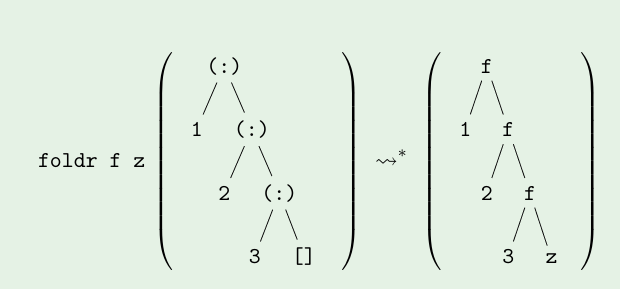
\includegraphics[width=\linewidth]{assets/foldr_grafico.png}
    \end{minipage}%
    \begin{minipage}[b]{0.5\textwidth}
        \centering
        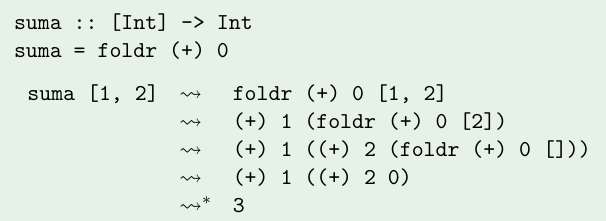
\includegraphics[width=\linewidth]{assets/suma_foldr.png}
    \end{minipage}
\end{figure}
Una función f está dada por recursión estructural sí: 
\begin{itemize}
    \item El caso base devuelve un valor fijo z.
    \item El caso recursivo es una función de x y (g xs)
    \item Se trabaja solamente con la cabeza de la lista.
    \item Se hace recursión sobre la cola pero no se tiene acceso a ella, sino al llamado recursivo.  Es decir, el caso recursivo no usa xs. 
    \item La recursión es la clásica, va desde derecha a izquierda. La R de foldr es de Right. 
\end{itemize}
Su estructura formal es la siguiente 
\begin{lstlisting}
    g [] = <caso base> -> valor 
    g (x:xs) = <caso recursivo> -> función cabeza de la lista y resultado de la recursión.
\end{lstlisting}
Por lo tanto foldr se define como
\begin{lstlisting}
    foldr :: (a -> (b -> b)) -> b -> [a] -> b 
    foldr f z [] = <
    foldr f z (x:xs) = f x (foldr f z xs)
\end{lstlisting}
\textbf{Importantísimo}: El tipado de foldr es $ Foldable \ t \implies (a \rightarrow b \rightarrow b) \rightarrow b \rightarrow t a \rightarrow b $
\begin{itemize}
    \item a = Es el elemento que tenemos actualmente en la recursión.
    \item b = Es cualquier tipo que nos permita acumular. Puede ser una tupla, un número, lo que sea. Pero en cada paso recursivo hay que llenar eso. El caso base tiene que cumplir este tipo b.
    \item Véase \hyperref[subsec:foldr_ejercicios]{\underline{\textbf{anexo}}} para ver ejemplos usando foldr.
\end{itemize}
¿Qué es lo que produce foldr (:) []? Es una identidad sobre listas porque haría recursión sobre una lista vacía. \\
¿Qué es lo que hace la siguiente función foldr? $ foldr(\backslash x \ r \rightarrow x) \ 0 \ [1, 2]$ 
\begin{itemize}
    \item Toma la lista y hace recursión. Empieza con el 2, ejecuta la función y devuelve 2. Hace el paso recursivo.
    \item Toma la lista y hace recursión. Ahora sigue con el 1, recibe 1 y la salida es 1. 
    \item Esta función agarra el primer elemento de una lista, sería el head.
\end{itemize}
\textbf{IMPORTANTÍSIMO}: Se pueden recorrer dos listas, tres listas, las que quieras a la vez con Foldr. La recursion se hace sobre una sola, pero las n-1 listas las enviarías por argumento en cada paso recursivo. Véase \hyperref[subsec:foldr_armar_pares]{\textbf{\underline{anexo}}} para ver ver el árbol de recursión y un ejemplo práctico. 
\textbf{Importante}: Foldr puede trabajar con listas infinitas. \\
Véase \hyperref[subsec:foldr_ex]{\textbf{\underline{anexo}}} para ver ejemplos de Foldr. \\
\subsection*{Recursión que \textbf{no} es estructural}
\begin{lstlisting}
    ssort :: Ord a => [a] -> [a]
    ssort [] = []
    ssort (x:xs) = minimo (x:xs) : ssort(sacarMinimo(x:xs))
\end{lstlisting}
No es estructural pues se esta usando xs para el llamado de minimo(x:xs) y no solamente en el llamado recursivo de ssort.
\subsection*{Iteración (foldl)}
Se la conoce como Plegado a la Izquierda porque va resolviendo inmediatamente de izquierda a derecha hasta que termine el proceso. \\
\begin{figure}[h]
    \centering
    \begin{minipage}[b]{0.5\textwidth}
        \centering
        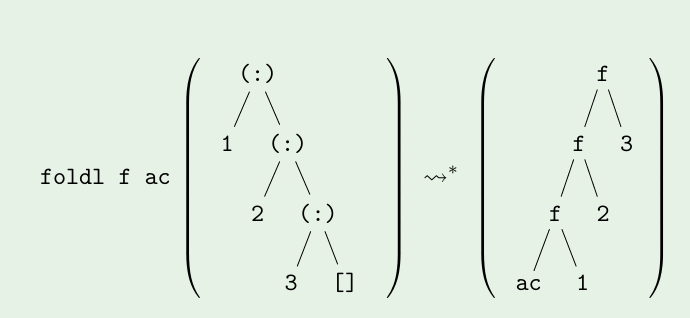
\includegraphics[width=\linewidth]{assets/foldl_grafico.png}
    \end{minipage}%
    \begin{minipage}[b]{0.5\textwidth}
        \centering
        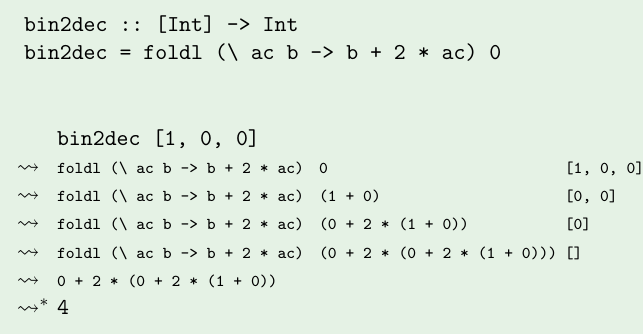
\includegraphics[width=\linewidth]{assets/bin2dec_foldl.png}
    \end{minipage}
\end{figure}
Este tipo de recursión es más que recursión una iteración, en este caso empezamos yendo desde el primer valor hasta el último. \\
En este enfoque voy modificando una solución parcial. \\
Por lo tanto foldl se define como
\begin{lstlisting}
    foldl :: (b -> a -> b) -> b -> [a] -> b 
    foldl f ac [] = ac
    foldl f ac (x:xs) = foldl f (f ac x) xs
\end{lstlisting}
¿Qué es lo que sucede en el siguiente ejemplo? \\
\begin{lstlisting}
    foldl (\x y -> 1) 0 unos
    foldl f (f 0 1) unos
    foldl f(f(f 0 1) 1) unos
\end{lstlisting}
Esto es in-realizable con foldl. Es decir, foldl no puede manejar listas infinitas. \\
\textbf{Importantísimo}: El tipado de foldl es $ Foldable \ t  \implies (b \rightarrow a \rightarrow b) \rightarrow b \rightarrow t a \rightarrow b $
\begin{itemize}
    \item b = Es cualquier tipo que nos permita acumular. Puede ser una tupla, un número, lo que sea. Pero en cada paso recursivo hay que llenar eso. El caso base tiene que cumplir este tipo b.
    \item a = Es el elemento que tenemos actualmente en la recursión.
\end{itemize}
Véase \hyperref[subsec:foldl_ejercicios]{\underline{\textbf{anexo}}} para ver ejemplos usando foldl.
\subsection*{¿Por qué foldl es peor que foldr?}
\textbf{foldl}: Procesa la lista de izquierda a derecha, lo que requiere evaluar toda la lista antes de devolver un resultado, lo que no es posible con listas infinitas. \\
\textbf{foldr}: Procesa la lista de derecha a izquierda, permite trabajar de manera perezosa y puede manejar listas infinitas si la función y el valor inicial permiten una evaluación parcial o completa sin necesidad de procesar todos los elementos.
\subsection*{Recursión Primitiva (recr)}
No existe en Haskell. Es una manera de nosotros podemos tener las mismas ventajas de foldr pero en este caso, la recursión primitiva nos permite utilizar la cola de la lista 
\begin{itemize}
    \item Se trabaja solamente con la cabeza de la lista y la cola.
    \item Se hace recursión sobre la cola.
\end{itemize}
Su estructura forma les la siguiente 
\begin{lstlisting}
    g [] = b
    g (x:xs) = f x xs (g xs)
\end{lstlisting}
Por lo tanto recr se define como 
\begin{lstlisting}
    recr :: (a -> [a] -> b ->b) -> b -> [a] -> b 
    recr f z [] = z
    recr f z (x:xs) = f x xs (recr f z xs)
\end{lstlisting}
\section*{Tipos}
Existen diferentes maneras de definir tipos. Esto es según sea el objetivo.
Definimos tipos con la palabra \textbf{data} + Nombre = Tipo1 | Tipo2 | Tipo 3 \\
Si hacemos en GHCI $:t Tipo1$ saldrá que es de tipo Nombre. \\
\textbf{Nota}: $|$ indica que a continuación hay otro tipo.
\subsection*{Tipos Comunes}
Son no recursivos, ej: $data Dia = Lu | Ma | Mi | Mie | Ju | Vi | Sa | Do $ \\
Lu, Ma, Mi, ... son constructores del tipo dia. \\
Los argumentos podrán ser recibidos diciendo qué tipo se espera, y usamos pattern matching para utilizarlos.
\begin{lstlisting}
    EsLunes :: Dia -> Bool
    EsLunes Lu = True 
    EsLunes _ = False 

    EsFinDeSemana :: Dia -> Bool
    EsFinDeSemana Sa = True 
    EsFinDeSemana Do = True 
    EsFinDeSemana _ = False 
\end{lstlisting}
\subsection*{Tipos con Funciones}
Los tipos también pueden tener tipos que necesiten argumentos. Difieren en la info que devuelven. \\
Ej.: data Persona = LaPersona String String Int \\
\textbf{Importante}
\begin{itemize}
    \item Si evaluamos $:t LaPersona$ sin enviar los argumentos retornará $LaPersona :: String -> String -> Int$. 
    \item Si evaluamos $:t LaPersona "T", "H", 23$ enviando los argumentos retornará que LaPersona es de tipo Persona
\end{itemize}
\begin{lstlisting}
    Edad :: Persona -> Int 
    Edad (LaPersona n a e) = e

    Cumpleaños :: Persona -> Persona 
    Cumpleaños (LaPersona n a e) = LaPersona n a (e+1)
\end{lstlisting}
\textbf{Importante}: Nótese que estamos devolviendo \textbf{una nueva persona}. En programación funcional no existe el concepto de "modificar" algo, sino crear algo nuevo con lo anterior y cambiarle algo.
\subsection*{Tipos Recursivos}
Cuando tengo tipos recursivos, las funciones que los usen deben manejar casos bases y la recursión \\
Ej.: data Nat = Zero | Succ Nat \\
\subsection*{Tipos Polimórficos} 
Al igual que las funciones, podemos definir que los tipos tengan constructores de un tipo específico.
\begin{lstlisting}
    data List a = Vacia | Const a (List a)
\end{lstlisting}
\subsection*{Importante en Tipos}
No se puede repetir un mismo constructor para un mismo tipo. \\
Es decir
\begin{lstlisting}
    data List = Vacia | Cons Int ListI 
    data List a = Vacia | Cost a (List a)

    Error. No puede estar Vacia como constructor de dos tipos diferentes.
\end{lstlisting}

\section*{Listas}
\begin{itemize}
    \item Por extensión: Es dar la lista implícita escribiendo todos sus elementos. Ej. [1, 2, 3]
    \item Secuencias: Progresiones aritméticas en un rango particular. Ej.: [3..7] es la lista que tiene los números del 3 al 7.
    \item Por compresión: Se definen de la siguiente manera [expresion | selectores, condiciones]. Ej.: [(x,y) | x <- [0..5], y <- [0..3], x+y==4] es la lista de pares que tienen elementos de x e y que dan menos que 4
\end{itemize}
\section*{Estructuras Recursivas sobre Otras Estructuras de Datos}
¿Cómo podemos plantear la estructura de un foldr para un árbol binario o cualquier estructura plegable que no sea una lista? \\
Lo primero que podemos intuir es que en las listas, solo hay una recursión, sobre la lista propiamente pero en un Árbol Binario tenemos dos caminos: rama izquierda y rama derecha. Esto quiere decirque de alguna manera, tenemos que capturar 2 recursiones.
\begin{itemize}
    \item Planteamos varios problemas acerca de esa estructura de datos y vemos qué patrones hay en común. 
    \item Las cosas que sean diferentes, las pasamos por parámetros. 
\end{itemize}
Por ejemplo, sean estas operaciones de un árbol binario 
\begin{lstlisting}
    nodos :: AB -> Int 
    nodos Nil = 0
    nodos (Bin i r d) = nodos i + 1 + nodos d 

    preorder :: AB -> [a]
    preorder Nil = []
    preorder (Bin i r d) = [r] ++ preorder i ++ preorder d
\end{lstlisting}
Podemos observar que cambia lo siguiente 
\begin{itemize}
    \item Tipos de salida: En el primer ejemplo devolvemos un int, en el segundo una lista de a. La lista de a sería el tipo que tenga el AB. 
    \item Caso base: En uno es [] y en otro 0. Por lo tanto tenemos que admitir un tipo b para el caso base. El caso base es del mismo tipo que el tipo de salida \textbf{siempre}.
    \item Función que realiza: En uno hace sumas, en el otro hace concatenaciones. 
\end{itemize}
¿Cómo podríamos escribir las funciones anteriormente mencionadas de manera anónima? 
\begin{lstlisting}
    nodos: (\ri r rd -> ri + 1 + rd)(nodos i) r (nodos d)
    preorder: (\ri r rd -> [r] ++ ri ++ rd) (preorder i) r (preorder d)
\end{lstlisting}
Recordemos la firma de foldr: $Foldable \ t \ \implies \ (a \ \rightarrow \ b \ \rightarrow \ b) \ \rightarrow \ b \ \rightarrow \ t \ a \ \rightarrow \ b$ \\
Donde b era el caso base / recursivo y a el elemento actual, acá tenemos dos. \\
Recordemos la estructura del tipo AB: AB a = Nil | Bin (AB a) a (AB a) \\
Entonces nuestra función foldAB va a tener que estar preparado para recibir ambos (AB a) y a.
foldAB :: (b $\rightarrow$ a $\rightarrow$ b $\rightarrow$ b) $\rightarrow$ b $\rightarrow$ AB a $\rightarrow$ b donde :t Bin: (AB a) $\rightarrow$ a $\rightarrow$ (AB) a $\rightarrow$ AB a donde 
\begin{itemize}
    \item $(b \rightarrow a \rightarrow b \rightarrow b)$
    \begin{itemize}
        \item la primera b: recursión rama izquierda
        \item la a: la raíz 
        \item la segunda b: recursión rama derecha 
        \item la tercera b: el resultado del proceso.
    \end{itemize}
    \item b: el resultado.
    \item AB a: la entrada 
    \item b: el resultado.
\end{itemize}
Es súper importante entender que la firma de la función que acepta foldAB está prácticamente atada al tipo de la estructura de dato.
\section*{Validación y Verificación de Programas}
\begin{itemize}
    \item Trabajaremos con estructuras de datos \textbf{finitas}. Más técnicamente, con tipos de datos \textbf{inductivos}.
    \item Trabajamos con \textbf{funciones totales}
    \begin{itemize}
        \item Las ecuaciones deben cubrir todos los casos posibles.
        \item La recursión siempre termina.
    \end{itemize} 
    \item El programa \textbf{no depende del orden} de las ecuaciones. 
\end{itemize}
\section*{Principio de Reemplazo}
Sea $e1 = e2$ una ecuación del programa. Las siguientes operaciones preservan la igualdad de expresiones.
\begin{itemize}
    \item Reemplazar \textbf{cualquier instancia} de e1 por e2.
    \item Reemplazar \textbf{cualquier instancia} de e2 por e1.
\end{itemize}
\textbf{Importante}: Si una igualdad se puede demostrar usando sólo el principio de reemplazo, decimos que la igualdad vale \textbf{por definición}.
\[\begin{minipage}[b]{0.9\textwidth}
    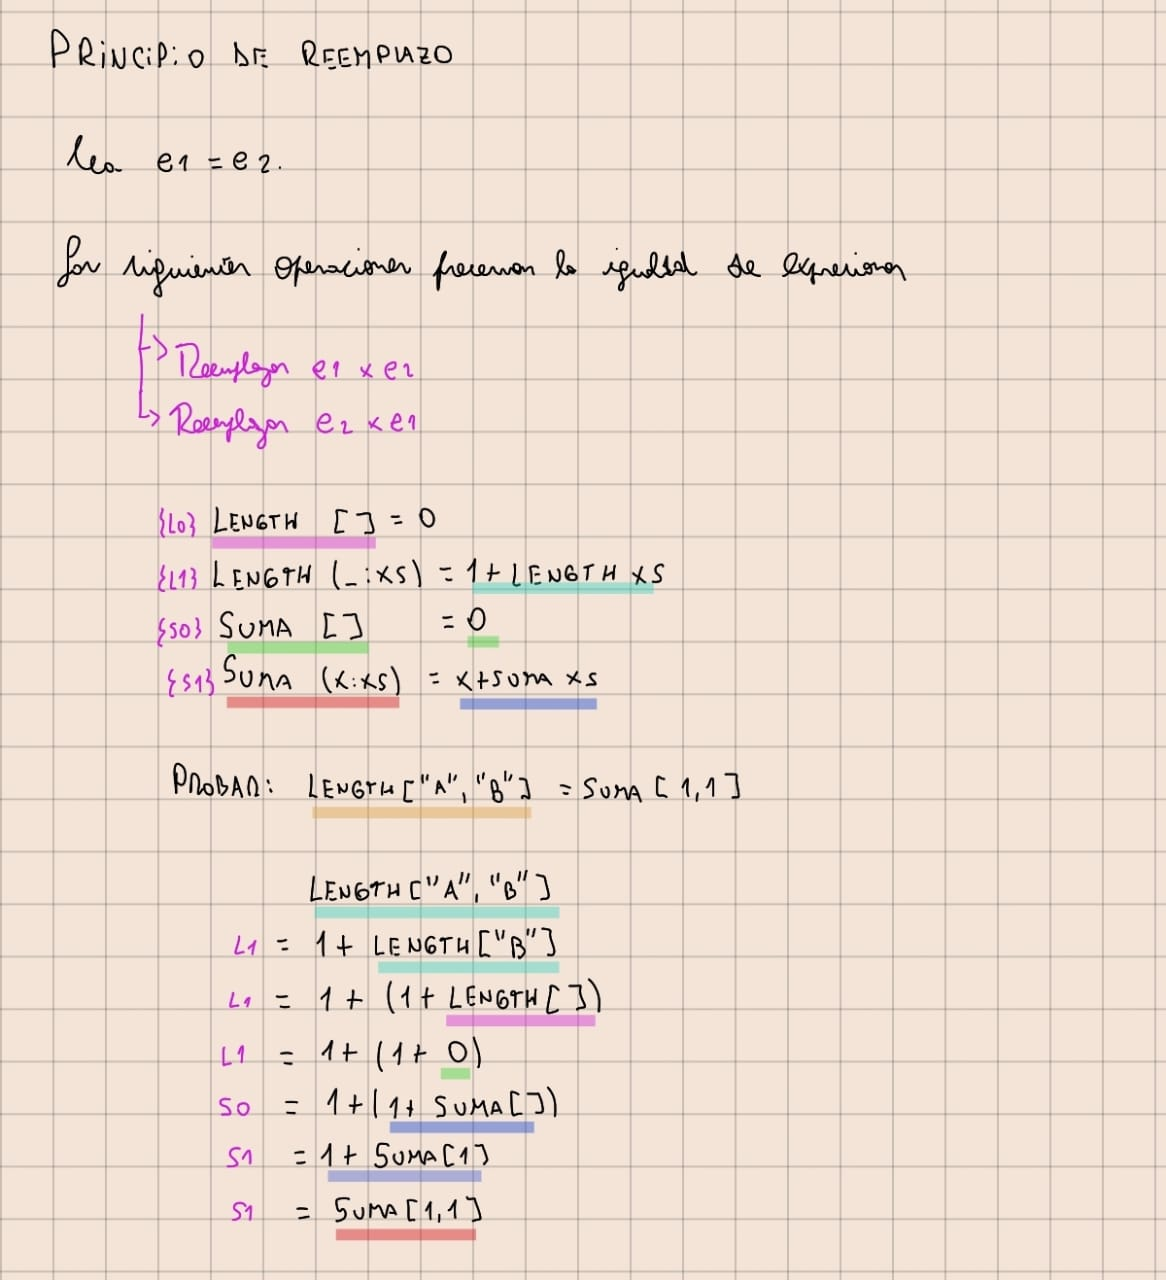
\includegraphics[width=\linewidth]{assets/principio_reemplazo_dibujo.jpg}
\end{minipage}\]
\section*{Inducción Estructural}
Cada tipo de datos tiene su propio principio de inducción. \\
\textbf{Importante}: El . acá cumple el rol del () en el $\forall$ es decir $\forall x :: Bool . \mathcal{P} \equiv (\forall x :: Bool)(\mathcal{P}) $ y el $::$ cumple el rol de \textbf{es del tipo...} \\
Los constructores de tipo NO recursivos serán los casos base mientras que aquellos constructores recursivos serán las hipótesis inductivas.
\subsection*{Formas de demostrar}
Existen 3 formas conocidas de demostrar cosas, por lo menos en la materia lo hacemos de maneras determinadas. Cuando usar una o la otra depende de la experiencia, y no es tan intuitivo saber cuando usar una opción u otra. 
\begin{itemize}
    \item Forma Álgebra: Arrancás desarrollando el lado izquierdo de tu TI. Aplicás la HI y tratás de llegar al lado derecho del TI.
    \item Forma Intermedia: Llegar de ambos lados de la TI a aplicar la HI. Solo funciona si estamos probando \textbf{igualdades}.
    \item Desarrollando lado derecho en base a contexto: Esta suele ser la opción más coherente en muchos casos. Consiste en desarrollar el TI del lado izquierdo, aplicar la HI y cuando llegamos a algo trivial o que no podemos seguir reduciendo, empezamos a desarrollar el lado derecho de la TI pero asumiendo las hipótesis del lado izquierdo. 
    \begin{itemize}
        \item Digamos que del lado izquierdo para aplicar la HI tuvimos que entrar a varios casos, por ejemplo: xs = (z:zs), e == z. Si llegamos a una respuesta trivial del lado izquierdo entonces desarrollamos el lado derecho asumiendo que xs tiene la pinta (z:zs) y efectivamente e == z. Esto nos hará todo mucho más corto.  
    \end{itemize}
\end{itemize}
Estas estrategias, las dejaré en el anexo para que claramente se note su diferencia y ventajas en cada caso. 
\subsection*{Inducción sobre booleanos}
Si $\mathcal{P}(True)$ y $\mathcal{P}(False)$ entonces $\forall x :: Bool \ \mathcal{P} (x)$ 
\[\begin{minipage}[b]{0.7\textwidth}
    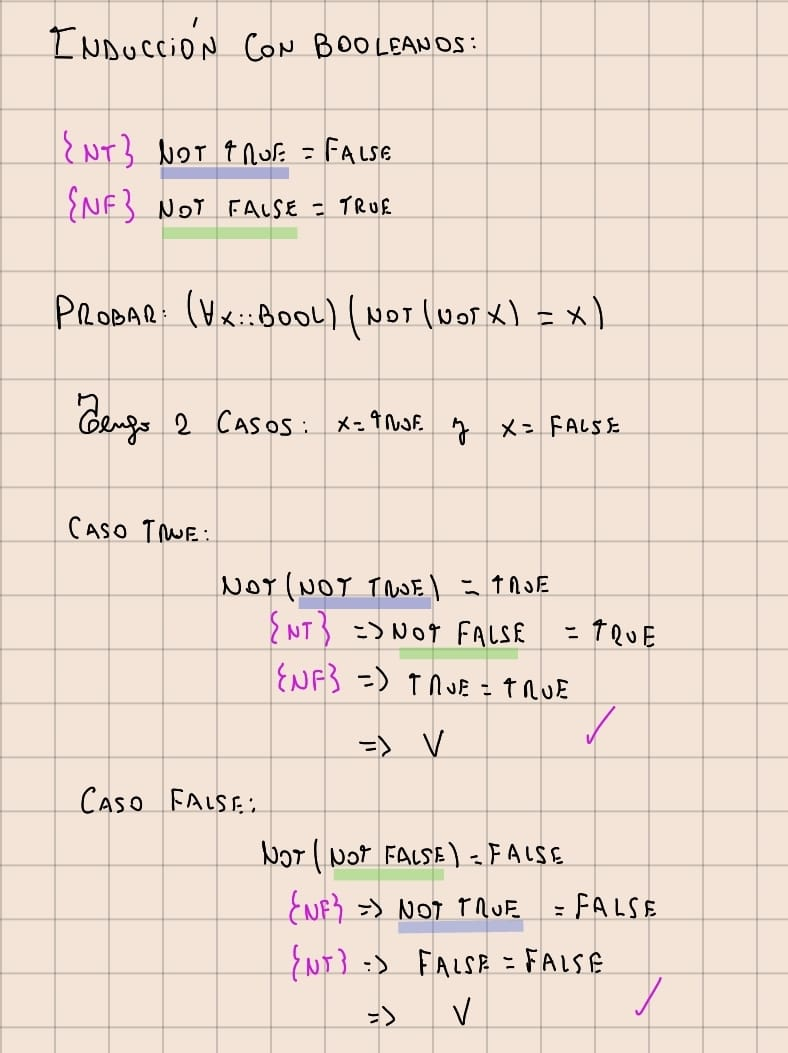
\includegraphics[width=\linewidth]{assets/induccion_booleanos_dibujo.jpg}
\end{minipage}\]
\subsection*{Inducción sobre pares}
Si $(\forall x :: a)(\forall y :: b)(\mathcal{P}(x, y))$ entonces $\forall p :: (a, b) \mathcal{P}(p)$
\[\begin{minipage}[b]{0.7\textwidth}
    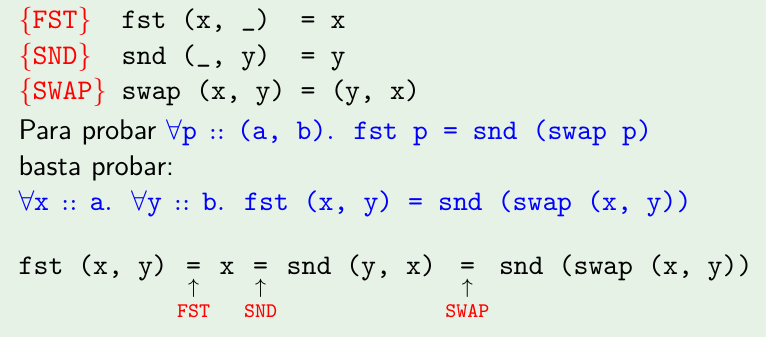
\includegraphics[width=\linewidth]{assets/induccion_pares.png}
\end{minipage}\]
\[\begin{minipage}[b]{0.7\textwidth}
    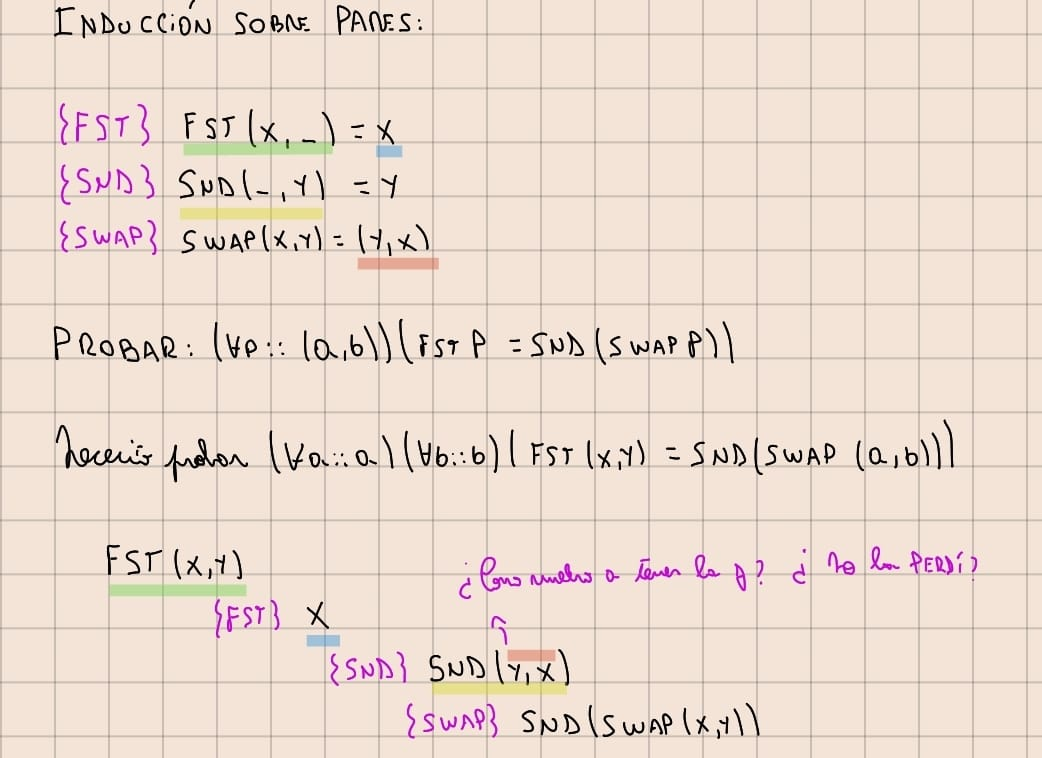
\includegraphics[width=\linewidth]{assets/induccion_pares_dibujo.jpg}
\end{minipage}\]
\subsection*{Inducción sobre naturales}
Si $\mathcal{P}(Zero)$ y $(\forall n :: Nat)(\mathcal{P}(n) \implies \mathcal{P}(Suc \ n))$ entonces $(\forall n :: Nat)(\mathcal{P}(n))$ donde 
\begin{itemize}
    \item $\mathcal{P}(n)$: Hipótesis Inductiva.
    \item $\mathcal{P}(Suc \ n)$: Tesis Inductiva.
\end{itemize}
\[\begin{minipage}[b]{0.7\textwidth}
    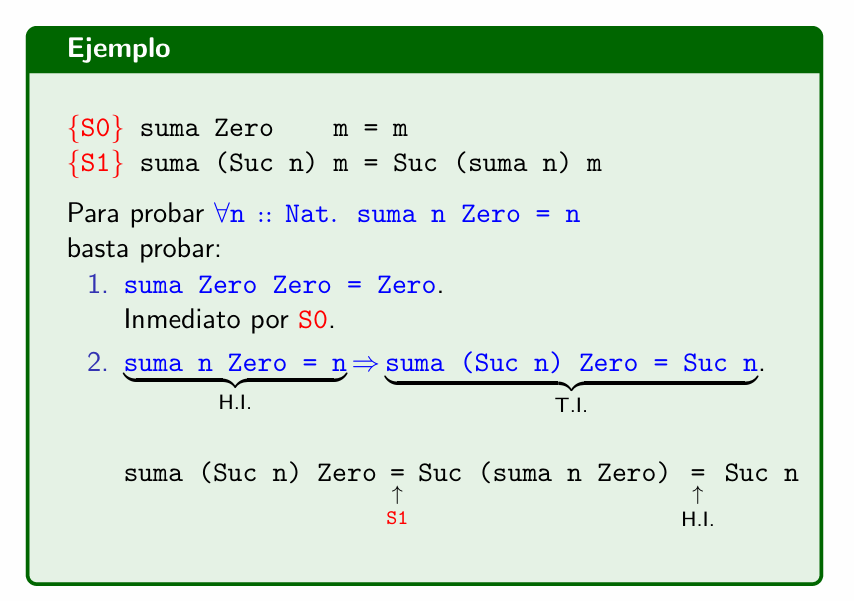
\includegraphics[width=\linewidth]{assets/induccion_naturales.png}
\end{minipage}\]
\[\begin{minipage}[b]{0.7\textwidth}
    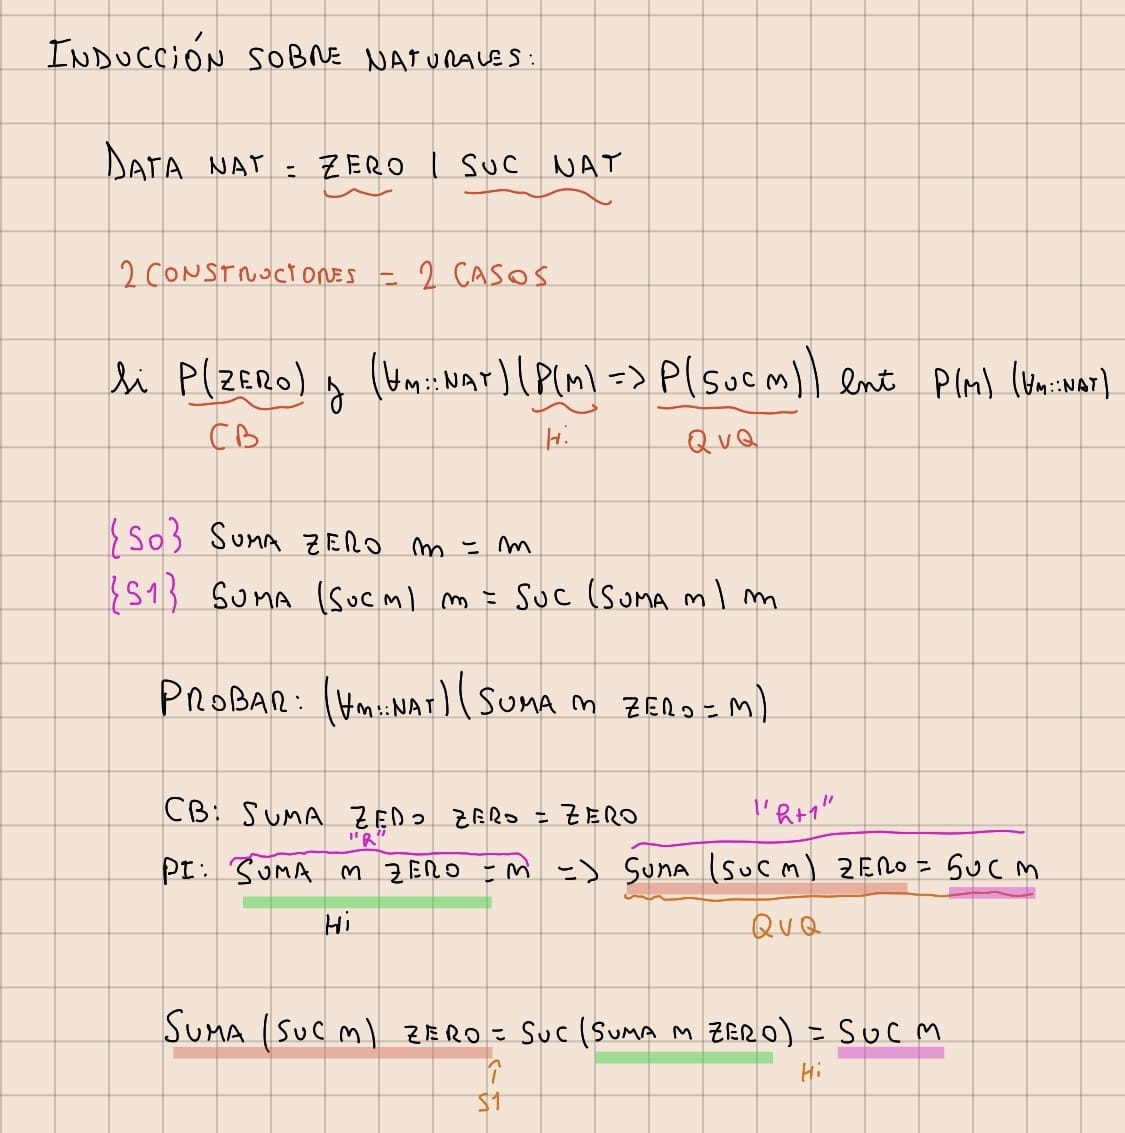
\includegraphics[width=\linewidth]{assets/induccion_naturales_dibujo.jpg}
\end{minipage}\]
\subsection*{Inducción Estructural: Caso General}
Sea $\mathcal{P}$ una propiedad acerca de las expresiones tipo T tal que 
\begin{itemize}
    \item $\mathcal{P}$ vale sobre todos los constructores base de T,
    \item $\mathcal{P}$ vale sobre todos los constructores recursivos de T, asumiendo como hipótesis inductiva que vale para los parámetros de tipo T,
\end{itemize}
entonces $(\forall x :: T)(\mathcal{P}(x))$
\subsection*{Principio de Inducción sobre Listas}
\[\begin{minipage}[b]{0.9\textwidth}
    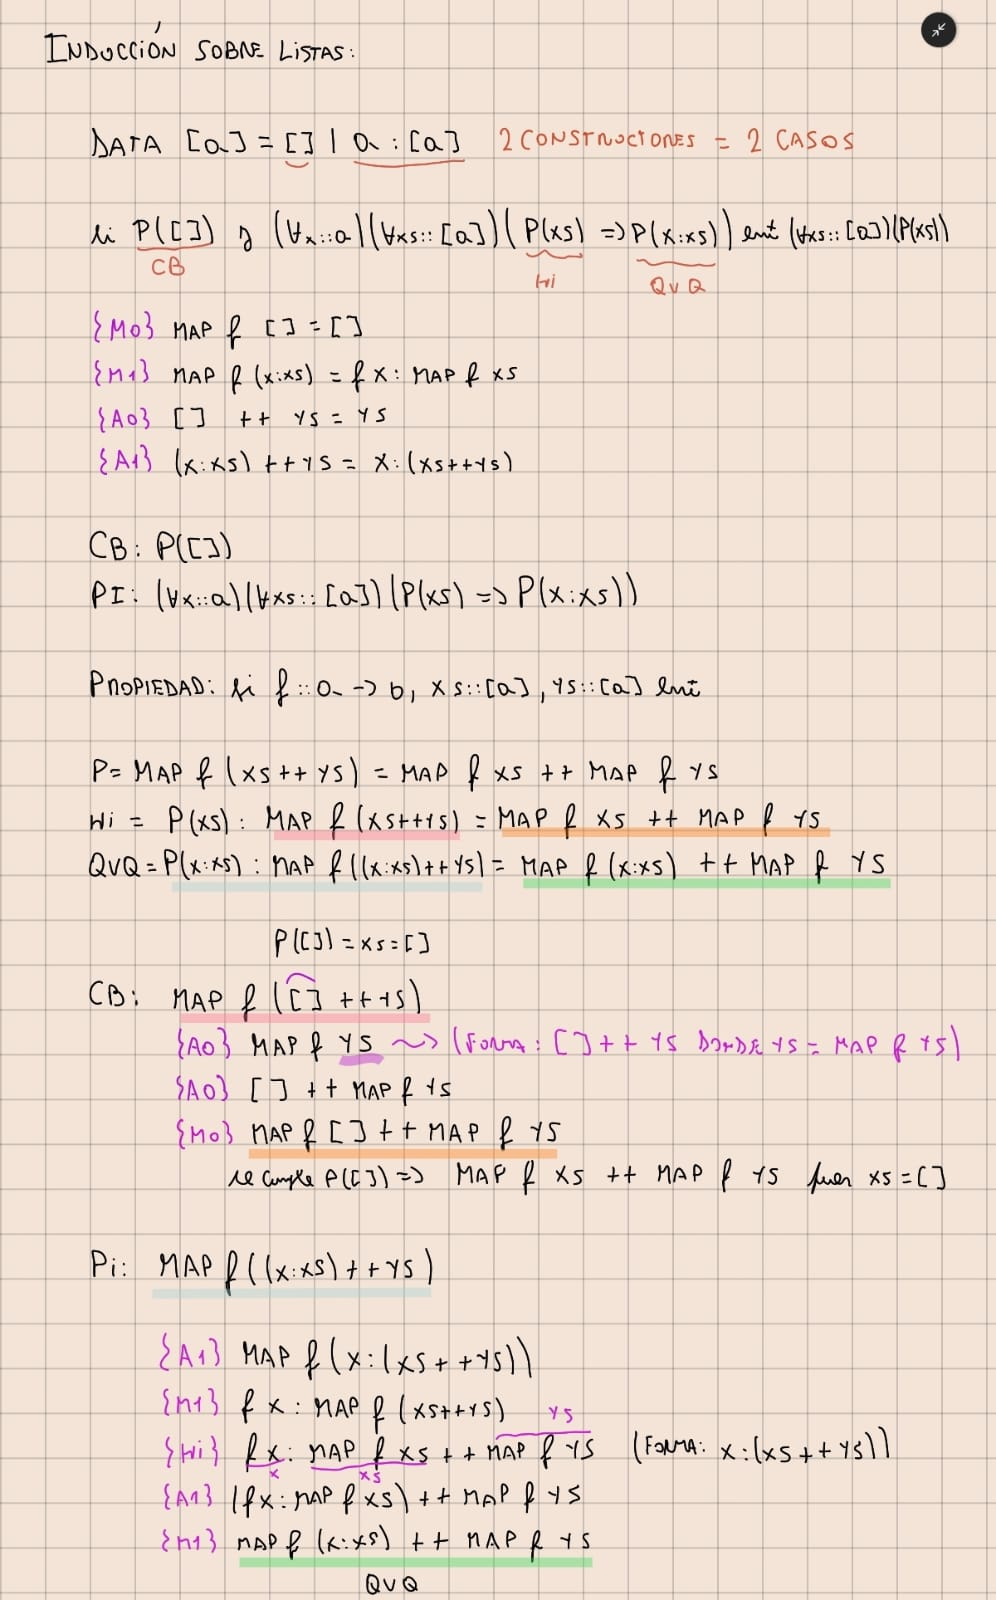
\includegraphics[width=\linewidth]{assets/induccion_listas_dibujo.jpg}
\end{minipage}\]
\subsection*{Principio de Inducción sobre Árboles Binarios}
\[\begin{minipage}[b]{0.7\textwidth}
    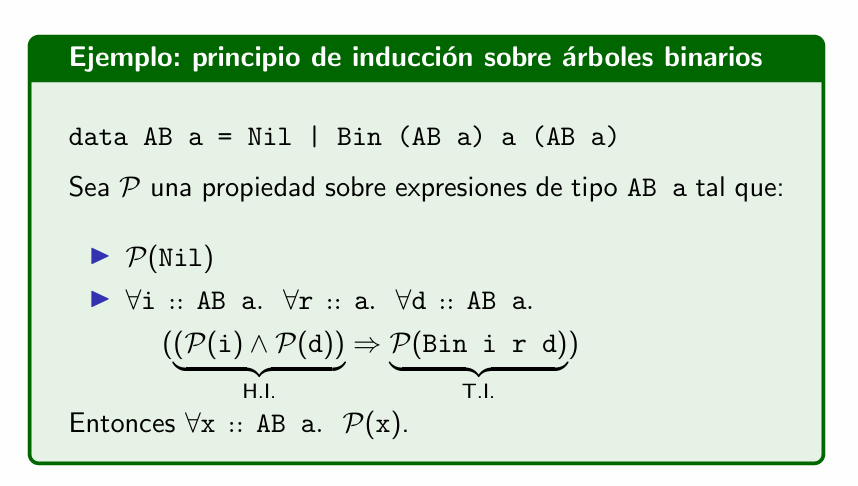
\includegraphics[width=\linewidth]{assets/principio_induccion_ab.png}
\end{minipage}\]
\subsection*{Principio de Inducción sobre Polinomios}
\[\begin{minipage}[b]{0.7\textwidth}
    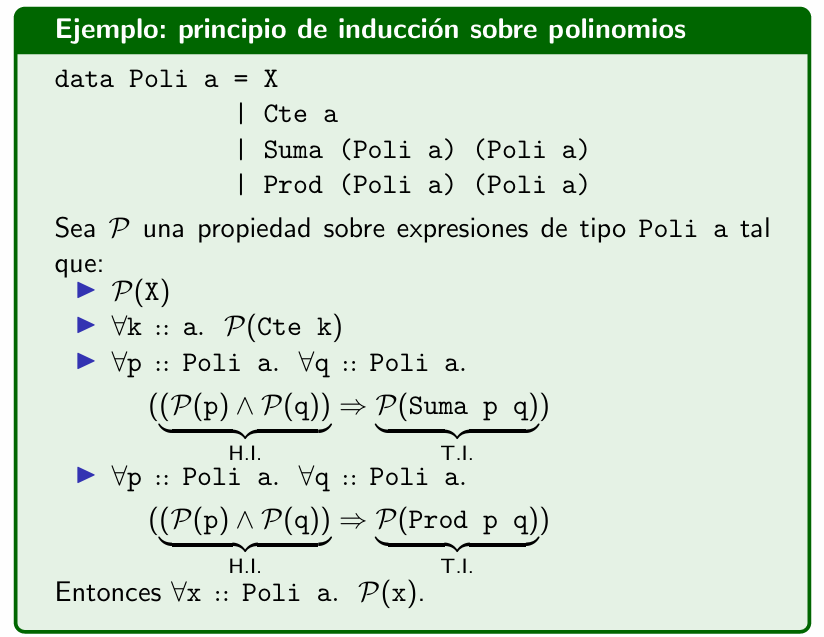
\includegraphics[width=\linewidth]{assets/principio_induccion_polinomios.png}
\end{minipage}\]
\subsection*{Relación entre foldr y foldl}
\textbf{Propiedad}: Si $f::a\rightarrow b \rightarrow b, \ z::b, \ xs::[a]$ entonces foldr f z xs = foldl (flip f) z (reverse xs) \\
\textbf{Lema}: Si $g::b \rightarrow a \rightarrow b, \ z::b, x::a, xs::[a]$ entonces foldl g z (xs ++ [x]) = g (foldl g z xs) xs
\subsection*{Puntos de vista intensional vs extensional}
Sí, es con \textbf{s}. Es intensional. \\
¿Es equivalente mergesort = insertionSort? La realidad es que: hacen lo mismo (llegan al mismo resultado); ordenan algo pero de una manera diferente.
\begin{itemize}
    \item Punto de vista intensional: Dos valores son iguales si están definidos de la misma manera.
    \item Punto de vista extensional: Dos valores son iguales si son indistinguibles al observarlos.
\end{itemize}
Entonces mergesort = insertionSort desde el lado extensional, porque hacen lo mismo pero no son iguales desde el punto de vista intensional. 
\subsection*{Principio de Extensionalidad Funcional}
Sean $f, \ g :: a \rightarrow b$. \\
\textbf{Principio de extensionalidad funcional}: Si $(\forall x :: a)(f \ x  =  g \ x) $ entonces $f=g$ \\
El ppio. de extensionalidad funcional nos dice que si son funciones son iguales entonces son iguales punto a punto donde las evaluemos.
\section*{Principio de Extensionalidad}
Nos permite predicar sobre la forma de algo particular y nos da la ventaja de poder seguir estudiando algo particular y poder sacar ciertas conclusiones. \\
\textbf{Importante}: Es súper común tener que aplicar este tipo de estrategias durante una demostración varias veces.   
\subsection*{Principio de Extensionalidad de Booleanos}
Dada una condición booleana, difurcamos en dos casos: o es verdadero, o es falso. \\
Ej.: $e == x$ se separa en dos casos 
\begin{itemize}
    \item e == x = true 
    \item e == x = false
\end{itemize}
\subsection*{Principio de Extensionalidad sobre Listas}
Dada una lista, que no sabemos que pinta tiene, podemos predicar sobre ella diciendo que tenemos dos casos 
\begin{itemize}
    \item xs = []
    \item $\exists z::a, z::[a] \ / \ xs = (z:zs)$
\end{itemize}
\subsection*{Demostración de Desigualdades}
¿Cómo demostramos que no vale una igualdad e1 = e2 :: A? \\
Entiendo que básicamente hay que encontrar hacer \textbf{ALGO} para demostrar que no son iguales. Este \textbf{ALGO} es una funcionalidad que devuelva algo con uno, y otra cosa con otro. Por lo tanto debería ser del tipo $obs \ a :: A \rightarrow Bool$. \\
Demostrar que \textbf{no} vale la igualdad: $id = swap :: (Int, Int) \rightarrow (Int, Int)$. \\
Esto es fácil de probar porque sabemos que $id$ nos da exactamente lo mismo que envíamos, y swap justamente da vuelta todo. Por lo tanto podemos comparar el primer elemento con id y el primer elemento haciendo el swap. \\
Ej.: $(1, 2) \rightarrow id (1, 2) \rightarrow (1, 2)$ pero $swap (1, 2) = (2, 1)$ y el primer elemento de $id (1, 2) \rightarrow (1, 2)$ es decir, $1 \neq 2$ que arroja el swap. \\
Por lo tanto
\begin{lstlisting}
    Ej: (1, 2)
    obs :: ((Int, Int) -> (Int, Int)) -> Bool 
    obs f = fst (f (1,2)) == 1

    obs id -> True 
    obs swap False
\end{lstlisting}
Nótese que el obs está \textbf{exactamente armado para este caso particular}. Para demostrar que las funciones no hacen lo mismo.
\section*{Isomorfismo de Tipos}
Decimos que dos tipos son isomorfos si podemos pasar de uno al otro aplicando alguna función y al componerlas el resultado arroja la función identidad. 
\begin{lstlisting}
    ("hola", (1, True)) :: (String, (Int, Bool))
    ((True, "hola"), 1) :: ((Bool, String), Int)
    Estos dos tipos son isomorfos porque podemos transformar los valores de un tipo en valores del otro

    f :: (String, (Int, Bool)) -> ((Bool, String), Int)
    f (s, (i, b)) = f((b, s), i)

    g :: ((Bool, String), Int) -> (String, (Int, Bool))
    g ((b, s), i) = f (s, (i, b))

\end{lstlisting}
¡Es básicamente crear una función que reciba los parámetros de otra manera y los mande a la otra función de la otra forma! Una especie de Curry/Uncurry. \\
Con esto se puede demostrar que $g . f = id$ y $f . g = id$ \\
Formalmente, podemos decir que dos tipos de datos A y B son \textbf{isomorfos} si 
\begin{itemize}
    \item Hay una función $f :: A \rightarrow B$ total.
    \item Hay una función $g :: B \rightarrow A$ total 
    \item Se puede demostrar que $g . f = id :: A \rightarrow A$
    \item Se puede demostrar que $f . g = id :: B \rightarrow B$
\end{itemize}
En criollo: Debe existir una función que me mapee de f a g y viceversa. Por último, si hago f(g) o g(f) tienen que dar la identidad. \\
\textbf{Notación}: $A \simeq B$ indican que A y B son isomorfos.
\section*{Sistemas Deductivos}
Sirve para razonar acerca de juicios (afirmaciones que queremos probar). \\
Ej.: Probar que \textbf{el tipo $(Bool \rightarrow Int)$} está sintácticamente bien formado 
\subsection*{Estructura de los Sistemas Deductivos}
Está dado por \textbf{reglas de inferencia} que tienen la siguiente estructura 
\begin{center}
    \barratexto{}{$\langle$ axioma $\rangle$}{$\langle$ nombre $\rangle$}
    \barratexto{$\langle premisa_{0} \rangle$ $\langle premisa_{1} \rangle$... $\langle premisa_{n} \rangle$}{$\langle$ nombre de la regla $\rangle $}{$\langle conclusion \rangle$}
\end{center}
\subsection*{Diferencia entre Axioma y Reglas de Inferencia}
\begin{itemize}
    \item \textbf{Axioma}: Es una afirmación que se asume como verdadera.
    \item \textbf{Reglas de Inferencia}: Permiten derivar afirmaciones (teoremas) a partir de axiomas y otras afirmaciones.
\end{itemize}
\subsubsection*{Cómo leer reglas de inferencia}
Existen dos formas, de abajo hacia arriba o de arriba hacia abajo.
\begin{itemize}
    \item De arriba hacia abajo: Si sabemos que valen las premisas, podemos decir que vale la conclusión.
    \item De abajo hacia arriba: Si queremos demostrar que vale la conclusión, tenemos que demostrar todas las premisas.
\end{itemize}
\subsection*{Árbol de Derivación} 
Es la representación gráfica de una derivación.
\begin{itemize}
    \item Los nodos representan afirmaciones.
    \item La raíz es la afirmación que se quiere probar.
    \item Las ramas representan las reglas de inferencias que conectan a las afirmaciones. 
\end{itemize}
Si llegamos a una prueba correcta, \textbf{las hojas son axiomas}.
\subsection*{Afirmación Derivable (Teorema)}
Una afirmación es derivable si existe alguna derivación sin premisas que la tiene como conclusión. \\
Es decir: si podés armar el árbol de derivación y llegás a hojas que son axiomas, entonces, tu afirmación es derivable.
\subsection*{Lógica Proposicional}
Dado un conjunto infinito de variables proposicionales: $\mathcal{P} = \{P, Q, R, \dots\}$
\subsubsection*{Fórmulas}
\begin{itemize}
    \item Cualquier variable proposicional es una fórmula.
    \item Si $\rho$ es una fórmula, entonces $\neg \rho$ es una fórmula.
    \item Si $\rho$ y $\sigma$ son fórmulas, $(\rho \land \sigma), (\rho \lor \sigma), (\rho \implies \sigma), (\rho \iff \sigma) $ son fórmulas.
\end{itemize}
Al ser un conjunto inductivo, viene provisto de 
\begin{itemize}
    \item Esquema de prueba para probar propiedades sobre ellos \textbf{inducción estructural}.
    \item Esquema de recursión para definir funciones sobre el conjunto \textbf{recursión estructural}.
\end{itemize}
\subsubsection*{Gramática de la Lógica Proposicional}
Las fórmulas son las expresiones que se pueden generar a partir de la siguiente gramática 
\[\tau, \sigma, \rho ... :: = P \ | \ \bot \ | \ (\tau \land \sigma) \ | \ (\tau \implies \sigma) \ | \ (\tau \lor \sigma) \ | \ \neg \tau\] 
Llamamos \textbf{contexto} a un conjunto finito de fórmulas.  \\
\textbf{Good to Know}
\begin{itemize}
    \item Los conectivos $\land, \lor$ no son conmutativos ni asociativos.
    \item La implicación, al igual que en Haskell, asocia a la derecha.
    \item Ómitimos los paréntesis más externos de las fórmulas.
    \item $\bot$ es siempre falso
\end{itemize}
\subsubsection*{Valuación}
Una valuación es una función $v : \mathcal{V} \implies \{V, F\}$ que asigna valores de verdad a las variables proposicionales. \\
Una valuación \textbf{satisface} una proposición $\tau$ si $ v \vDash \tau$ donde: 
\begin{itemize}
    \item $v \vDash P \ sii \ v(P) = V$
    \item $v \vDash \neg \tau \ sii \ v \nvDash \tau$
    \item $v \vDash \tau \lor \sigma \ sii \ v \vDash \tau \ o \ v \vDash \sigma$
    \item $v \vDash \tau \land \sigma \ sii \ v \vDash \tau \ y \ v \vDash \sigma$
    \item $v \vDash \tau \implies \sigma \ sii \ v \nvDash \tau \ o \ v \vDash \sigma$
     \item $v \vDash \tau \iff \sigma \ sii \ v \vDash \tau \ sii \ v \vDash \sigma$
\end{itemize}
\textbf{Nota}: Una valuación es una fila de la tabla de verdad. Es decir, cada variable se le asigna un valor de verdad para esa valuación. \\ 
Ej.: Si tengo $\sigma \land \tau$ ¿qué necesito que pase para $\sigma$ y $\tau$ para que sea verdadero? Bueno, necesito que la valuación de $v \vDash \sigma$ y $v \vDash \tau$ \\
A modo de ejercicio escribamos uno de estas valuaciones con árboles de derivación a nivel de sistema deductivo: 
\begin{center}
    \barratexto{$v \vDash \tau \ v \vDash \sigma$}{$\langle$ $v \vDash \tau \land \sigma $ $\rangle$}{$\langle$ $\land$ $\rangle$}
\end{center}
\subsubsection*{Contexto}
Es un conjunto finito de fórmulas. Es lo que tenemos como información en nuestros juicios a medida que vamos encontrando las premisas. \\
Ej.: $\Gamma = P \implies Q, \neg Q$
\subsubsection*{Semántica en Lógica Proposicional}
Una valuación v satisface un contexto $\Gamma$ $(v \vDash \Gamma)$ sí y solo sí v satisface todas las fórmulas de $\Gamma$. \\
Si $\Gamma = P \land Q, \neg Q$ entonces para que $v \vDash \Gamma$ tiene que suceder que: 
\begin{itemize}
    \item $v \vDash P \land Q$ sii $v \vDash P$ y $v \vDash Q$
    \item $v \vDash \neg Q$ sii $v \nvDash Q$
\end{itemize}
\textbf{Good to Know}: Todo v satisface al contexto vacío. \\
\textbf{Consecuencia Lógica}: Si llegase a encontrar ahora una fórmula $\tau$ del conjunto $\Gamma (\Gamma \vDash \tau)$, entonces, todas las valuaciones $v$ que valían en $\Gamma$, valen también en $\tau$ (si antes valía, y ahora agregué $\tau$ veo que siga valiendo).
\subsubsection*{Equivalencia Lógica y Tipos de Fórmulas}
Dadas dos fórmulas $\tau$ y $\sigma$: 
\begin{itemize}
    \item $\tau$ es lógicamente equivalente a $\sigma$ cuando $v \vDash \tau$ sii $v \vDash \sigma$ para toda valuación $v$.
\end{itemize}
Una fórmula $\tau$ es: 
\begin{itemize}
    \item Una tautología si $v \vDash \tau$ para toda valuación $v$. 
    \item Satisfactible si existe una valuación $v$ tal que $v \vDash \tau$
    \item Insatisfactible si no es satisfactible.
\end{itemize}
Un conjunto de fórmulas $\Gamma$ es 
\begin{itemize}
    \item Satisfactible si existe una valuación $v$ tal que $\forall \tau \in \Gamma$ se tiene $v \vDash \tau$
    \item Insatisfactible si no es satisfactible.
\end{itemize}
\subsubsection*{Teorema de la Insatisfactibilidad}
Una fórmula $\tau$ es una tautología sii $\neg \tau$ es insatisfactible.
\subsection*{Sistema Deductivo (Deduccion Natural)}
El enfoque que vimos antes de la lógica proposicional a través de la semántica tiene algunas limitaciones. \\
En nuestro caso, vemos el sistema de deducción natural aunque existen otros. \\
Este sistema trabaja con afirmaciones (juicios) de la forma $\Gamma \vdash \tau$ donde $\Gamma$ es la hipótesis y $\tau$ es la tesis.
\subsubsection*{Lógica Intuicionista (NJ) vs Lógica Clásica (NK)}
Las reglas de la lógica intuicionista están contenidas en las reglas de la lógica clásica. \\
Algunas reglas que podemos aplicar en la \textbf{lógica clásica} que no podemos usar en la lógica intucionista 
\begin{itemize}
    \item PBC (proof by contradiction): No es derivable, es decir, no se puede deducir.
    \item LEM (law of excluded middle): Es un axioma, no tiene premisas y por lo tanto no se puede probar.
    \item $\neg \neg e$ (doble negation elimination)
\end{itemize}
Las reglas \textbf{PBC}, \textbf{LEM} y \textbf{$\neg \neg e$} son equivalentes.
\[\begin{minipage}[b]{0.7\textwidth}
    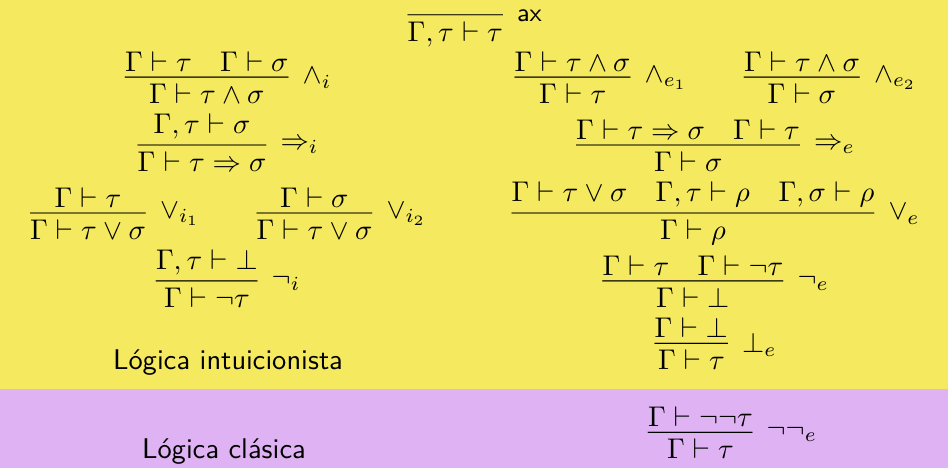
\includegraphics[width=\linewidth]{assets/logica_1.png}
\end{minipage}\]
\[\begin{minipage}[b]{0.7\textwidth}
    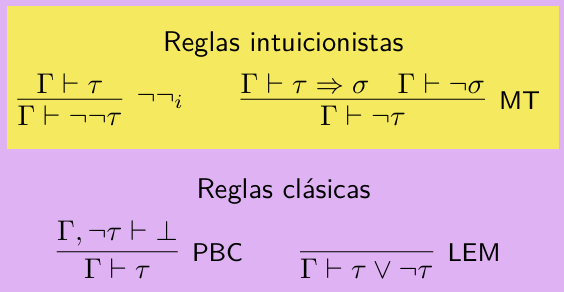
\includegraphics[width=\linewidth]{assets/logica_2.png}
\end{minipage}\]
Si un juicio es derivable en NJ también lo es en NK, esto se debe a que NJ es más restrictivo que NK. \\
¿Por qué es importante NJ? Porque es la base de un lenguaje de programación funcional.
\subsection*{Weakening (Debilitamiento) y Strengthening (Fortalecimiento)}
\subsubsection*{Weakening}
Si $\Gamma \vdash \tau$ es derivable, entonces $\Gamma, \sigma \vdash \tau$ es derivable. 
\subsubsection*{Strengthening}
Es lo contrario a Weakening, la idea es que podemos ir sacando hipótesis que no nos sirven y poder seguir probando que vale. Se utiliza mucho en algo llamado Cálculo Lambda que veremos luego. \\
Se dice que es Strengthening porque estamos haciendo más fuerte la prueba, esto es porque a menor cantidad de información que tiene el contexto es más fácil de probar.
\subsection*{Correctitud (Soundness) y Completitud}
\textbf{Importante}: Utilizamos $\vDash$ para hablar de satisfacibilidad en el contexto de \textbf{semántica} mientras que utilizamos $\vdash$ para indicar que una fórmula se puede derivar en el contexto de \textbf{sintáxis}. \\

Correctitud y Completitud responde a la siguiente pregunta: ¿cuál es la relación entre la sintáxis y la semántica?
\begin{itemize}
    \item \textbf{Sintáxis}: Conjunto de fórmulas $\tau$ tal que $\neg \tau$ es un secuente válido. 
    \item \textbf{Semántica}: Conjutno de fórmulas $\tau$ tal que $v \vDash \tau$ para toda valuación $v$. Ej: Tautologías.
\end{itemize}
\[\Gamma \vDash T \iff \Gamma \vdash T\]
\textbf{Corrección} \\
$\vDash \tau$ secuente válido implica que $\tau$ es tautología.
\begin{itemize}
    \item $\sigma_{1}, \sigma_{2}, \dots, \sigma_{n} \vdash \tau$ secuente válido implica que $\sigma_{1}, \sigma_{2}, \dots, \sigma_{n} \vDash \tau$
\end{itemize}
\textbf{Para demostrar}: Hacemos inducción en la estructura de la prueba analizando por casos la última regla aplicada en la prueba. \\
Caso base, la última regla fue un axioma. \\
Casos recursivos, el resto de reglas $\land_{i}, \land_{e1}, etc$ \\
\textbf{Completitud}
$\tau$ tautología implica que $\vdash \tau$ es secuente válido. 
\begin{itemize}
    \item $\sigma_{1}, \sigma_{2}, \dots, \sigma_{n} \vDash \tau$ implica que $\sigma_{1}, \sigma_{2}, \dots, \sigma_{n} \vdash \tau$ es un secuente válido. 
\end{itemize}
\textbf{Para demostrar}: Usamos el contrarrecíproco: si $P \implies Q$ vale que $\neg Q \implies \neg P$ \\
Luego probar estos dos lemas
\begin{itemize}
    \item Si $\Gamma \nvdash \tau$ entonces $\Gamma \cup \{\neg \tau\}$ es consistente (sale por contrarrecíproco).
    \item Si $\Gamma$ es consistente, entonces tiene modelo. Ej.: $\Gamma$ es satisfactible (es más dificil).
\end{itemize}
\subsection*{Consecuencia Semántica}
Sean $\tau_{1}, \tau_{2}, \dots, \tau_{n}, \sigma$ fórmulas de la lógica proposicional. \\
$\tau_{1}, \tau_{2}, \dots, \tau_{n} \vDash \sigma \iff \forall \ v \ valuacion \ ((v \vDash \tau_{1} \land v \vDash \tau_{2} \land \dots \land v \vDash \tau_{n}) \implies (v \vDash \sigma))$ \\
\textbf{En criollo}: Vale que $\tau_{1}, \tau_{2}, \dots, \tau_{n} \vDash \sigma \iff$ para toda valuación v tal que v satisface a todas las hipótesis $v \vDash \tau_{i}$ para toda $i \in 1, \dots, n \implies v \vDash \sigma$ 
\subsection*{Consistencia}
Decimos que $\Gamma$ es consistente si $\Gamma \nvdash \bot$, es decir, $\Gamma$ es consistente si no se puede derivar una contradicción a partir de él.
\section*{Cálculo Lambda ($\lambda$)}
Es un lenguaje de programación. Puede computar cualquier cosa. En lenguajes funcionales hablamos de cálculo lambda mientras que en lenguajes imperativos hablamos de máquinas de Turing. \\
Para entrar en calor, comenzaremos hablando del cálculo lambda no tipado. Luego, introduciremos la noción de tipos.
\subsection*{Reglas Generales}
Es probable que muchas cosas que mencione acá no se hayan definido todavía, pero ténganlo presente a medida que lean el documento. Esto, más que nada, para que las reglas más importantes estén en un único lugar. 
\begin{itemize}
    \item La aplicación es asociativa a izquierda.
    \begin{itemize}
        \item $M N R = (M N) \ R$
    \end{itemize}
    \item El constructor de tipos $\rightarrow$ es asociativo a derecha.
    \begin{itemize}
        \item $\tau \rightarrow \sigma \rightarrow \rho = \tau \rightarrow (\sigma \rightarrow \rho)$
    \end{itemize}
    \item La aplicación tiene mayor precedencia (se resuelve primero) que la abstracción, y que el condicional. (APP > ABS > COND)
    \begin{itemize}
        \item if x then y else z true $\equiv$ if x then y else (z true). 
        \item $\lambda x:\tau$. if x then y else z  $\equiv$ $\lambda x:\tau.$(if x then y else z). 
        \item $\lambda x:\tau .$ if x then y else z true $\stackrel{APP}{=}$ $\lambda x:\tau.$ if x then y else (z true) $\stackrel{ABS}{=}$ $\lambda x:\tau. $(if x then y else (z true)). 
    \end{itemize}
    \item fv(M): Es el conjunto de variables libres de \textbf{cada posible término M} de un sistema de tipos. Una variable está ligada si está al alcance de una abstracción.
    \item Todas las funciones toman un único argumento. 
    \begin{itemize}
        \item $\lambda x.\lambda y. \lambda z.$(if x then y else z) genera (if x then y else z) con los argumentos ya aplicados.
    \end{itemize}
\end{itemize}
\subsection*{Con booleanos}
Los términos válidos de cálculo lambda con booleanos los podemos describir con una gramática formal 
\[
\begin{aligned}
M \ ::= \ & x \quad &&\text{(variable)} \\
       | \ & \lambda x .\ M \quad &&\text{(abstracción)} \\
       | \ & M\ N \quad &&\text{(aplicación)} \\
       | \ & \text{true} \quad &&\text{(constante verdadera)} \\
       | \ & \text{false} \quad &&\text{(constante falsa)} \\
       | \ & \text{if } M \text{ then } N \text{ else } P \quad &&\text{(condicional)}
\end{aligned}
\]
\begin{itemize}
    \item \textbf{Tipos}: $\tau, \sigma, \rho, \dots ::= bool \ | \ \tau \rightarrow \sigma$. 
    \item \textbf{Términos}: Variables $X = \{X, Y, Z, \dots\}$
\end{itemize}
\subsection*{Cálculo Lambda tipado}
En el Cálculo Lambda tipado damos los tipos en las operaciones, ej.: $\backslash \lambda x:\sigma \ . \ M$
\subsection*{Función Identidad}
En cálculo lambda existe una función id \textbf{propia por cada tipo}.
\subsubsection*{Captura de variables ($\alpha$ equivalencias)}
Decimos que dos términos M y N son $\alpha$ equivalentes si solamente difieren en el nombre de sus variables ligadas.\\
Ej.: $\lambda x.\lambda y.x = \lambda y.\lambda x.x$
\subsubsection*{Conjunto de Variables Libres $fv(M)$}
El conjunto de variables libres de un término M se define para todo posible término del sistema de tipos y se denota como $fv(M)$. \\
Definamos, para cada término del cálculo lambda en booleanos el conjunto de variables libres
\begin{itemize}
    \item $fv(x) \stackrel{def}{=} \{x\}$
    \item $fv(\lambda x. M) \stackrel{def}{=} fv(M) \backslash \{x\}$
    \item $fv(true), fv(false) \stackrel{def}{=} \emptyset$
    \item $fv(M N) \stackrel{def}{=} fv(M) \cup fv(N)$
    \item $fv(if \ M \ then \ N \ else \ P) \stackrel{def}{=} fv(M) \cup fv(N) \cup fv(P)$
\end{itemize}
Si $fv(M) = \emptyset$ entonces $M$ es \textbf{cerrado} es decir, no tiene variables libres.
\subsection*{Sistema de Tipos}
Se formaliza con un sistema deductivo. Solo tipamos términos sin variables libres. Indica \textbf{cómo se construyen los programas.}
\subsubsection*{Contexto de tipado}
¿Qué sucede con el siguiente programa? $(\lambda x:Bool. (y \ x))$ \\
Como y puede (o no) tener variables libres, necesitamos un \textbf{contexto de tipado}.\\
Un contexto de tipado es un conjunto finito de pares $(x_{i}:\tau_{i}): \{x_{1}:\tau_{1}, \dots, x_{n}:\tau_{n}\}$ \textbf{sin variables repetidas} $(i \neq j \implies x_{i} \neq x_{j})$ \\
A veces notamos $dom(\Gamma) = \{x_{1}, \dots, x_{n}\}$, por lo que, si queremos saber el tipo de $x_{i}$, podemos escribir $\Gamma(x_{i})$ \\
Decimos que el contexto de tipado está vacío $(\emptyset)$ cuando \textbf{o bien el término no tiene ninguna variable libre o bien cuando el término es una constante}
\subsubsection*{Juicios de Tipado}
El sistema de tipos predica sobre \textbf{juicios de tipado} de la forma: $\Gamma \vdash M:\tau$ \\
Se lee como ``en el contexto $\Gamma$, $M$ es de tipo $\tau$``
\[\begin{minipage}[b]{1\textwidth}
    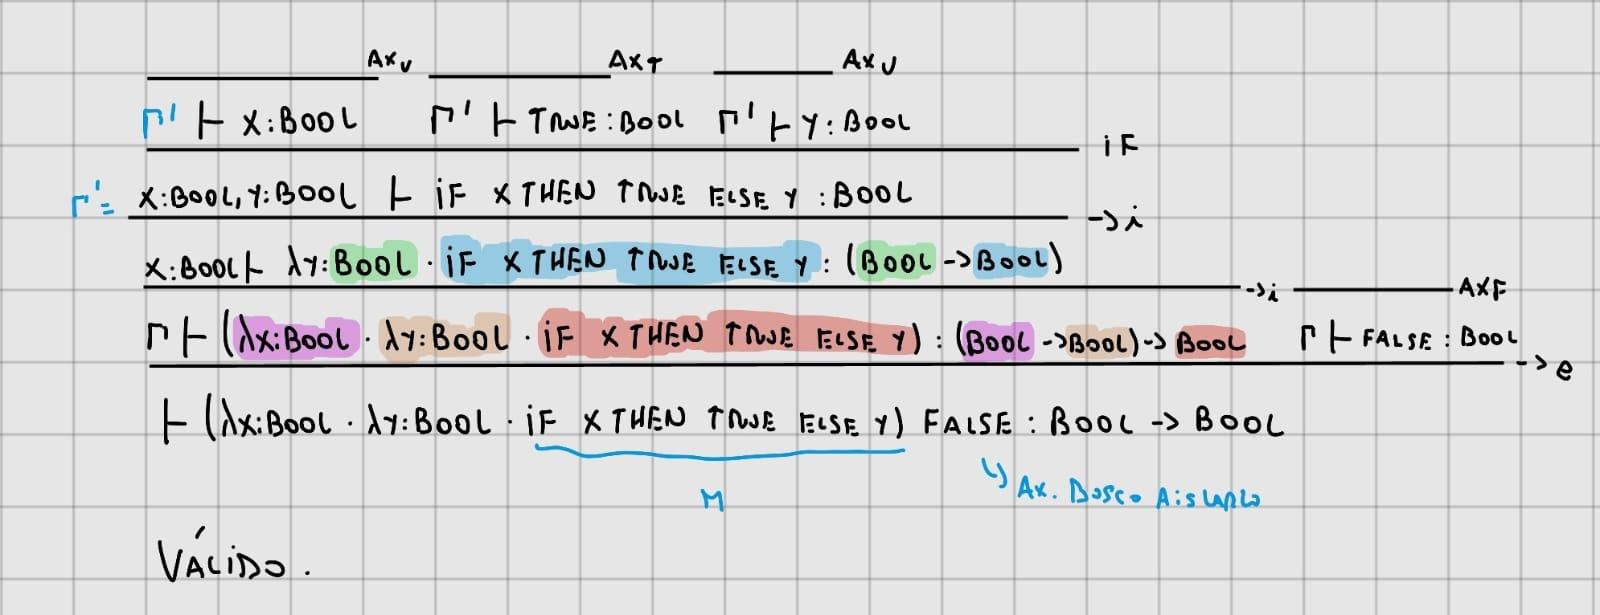
\includegraphics[width=\linewidth]{assets/tipado.jpg}
\end{minipage}\]
\subsubsection*{Reglas de tipado}
\[\begin{minipage}[b]{0.7\textwidth}
    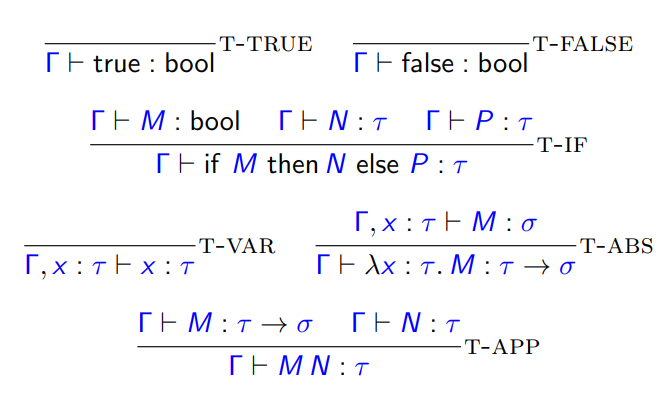
\includegraphics[width=\linewidth]{assets/tipado_operaciones2.png}
\end{minipage}\]
\subsubsection*{Unicidad de Tipos}
Si $\Gamma \vdash M:\sigma$ y $\Gamma \vdash M:\rho$ son derivables ent $\sigma = \rho$ \\
\textbf{Importante}: No vale en todos los sistema de tipos, pero vale en el cálculo lambda tipado y es fundamental.
\subsubsection*{Teorema (Weakening + Strengthening)}
Si $\Gamma \vdash M:\tau$ es derivable y $fv(M) \subseteq \Gamma \cap \Gamma'$ entonces $\Gamma' \vdash M:\tau$ es derivable
\begin{itemize}
    \item Weakening: Agregar más hipótesis hace que la afirmación sea más débil y dificil de demostrar.
    \item Strengthening: Sacar hipótesis hace que la afirmación sea más fuerte y fácil de demostrar.
\end{itemize}
Lo importante es acordarse que
\begin{itemize}
    \item Si en el contexto tenés algo que te sirve para tipar en M, entonces podés agregar cuantas cosas quieras en el contexto que va a seguir valiendo (weakening). 
    \item Si en el contexto tenés algo que NO te sirve para tipar en M, entonces podés sacarlo que no te va a afectar en nada (strengthening).
\end{itemize}
\subsubsection*{Tipos Habitados}
Uu tipo está habitado si existe un término M tal que el juicio $\vdash M:\tau$ es derivable. \\
Por ejemplo, si nos piden algo que cumpla $\vdash M:(\tau \rightarrow \rho) \rightarrow (\sigma \rightarrow \tau) \rightarrow (\sigma \rightarrow \rho)$. \\
Podemos notar que una función que haga esto, sería la composición: $\lambda f:\tau \rightarrow e . \lambda g :\sigma \rightarrow \tau . \lambda x:\sigma . f (gx)$ o mejor escrita $(\lambda f:\tau \rightarrow e) (\lambda g :\sigma \rightarrow \tau)(\lambda x:\sigma) (f (gx))$
\subsection*{Semántica Formal}
Nos permite darle significado a nuestros programas.
\begin{itemize}
    \item \textbf{Semántica Operacional}: Indica cómo se ejecuta el programa hasta llegar a un resultado. Es el tipo de semántica que usamos en la materia que trabaja en base a reglas de reducción entre términos. La idea es llegar a expresiones irreducibles.
    \begin{itemize}
        \item small-step: ejecución paso a paso.
        \item big-step: evaluación directa al resultado.
    \end{itemize}
    \item \textbf{Semántica Denotacional}:  Interpreta los programas como objetos matemáticos.
    \item \textbf{Semántica Axiomática}: Establece relaciones lógicas entre el estado del programa antes y después de la ejecución.
\end{itemize}
\subsubsection*{Forma Normal}
Un término está en forma normal cuando no existe ninguna regla que lo reduzca a otro.
\subsubsection*{Determinismo}
Cuando cada término que \textbf{NO} está en forma normal tiene una única forma de reducir.
\subsubsection*{Estrategia de Reducción}
Usaremos la estrategia de reducción \textbf{call by value}. \\
$M \rightarrow N$: indica que M reduce o reescribe a N. 
\subsubsection*{Programa}
Es un término M tipable y cerrado (fv(M) = $\emptyset$) que debe ser derivable para algún $\tau$. 
\subsubsection*{Juicios de Evaluación}
La semántica operacional hace afirmaciones sobre juicios de evaluación $M \rightarrow N$ donde M y N son programas.
\subsubsection*{Valores}
Los valores son los posibles resultados de evaluar programas, se definen como los términos cerrados y bien tipados V producidos por la gramática de valores. \\
La estrategia call-by-value define los siguientes valores: $V ::= true \ | \ false \ | \ \lambda x:\sigma.M$, estos ya tienen todos sus parámetros completamente reducidos, de lo contrario, no serían valores. \\
\textbf{Ej.}: $V ::= \ \dots \ | \ Nil \ | \ Bin(V, V, V)$ corresponde a los valores de trabajar con un árbol binario. 
\subsubsection*{Obtener Valores}
Para poder obtener valores, debemos ir reduciendo las expresiones. Depende de qué sistema de tipos y operaciones tengamos, cada una tiene su forma de reducirse. \\
A continuación, se demuestran las reglas de reducción para las expresiones booleanas y funciones. 
\[\begin{minipage}[b]{0.9\textwidth}
    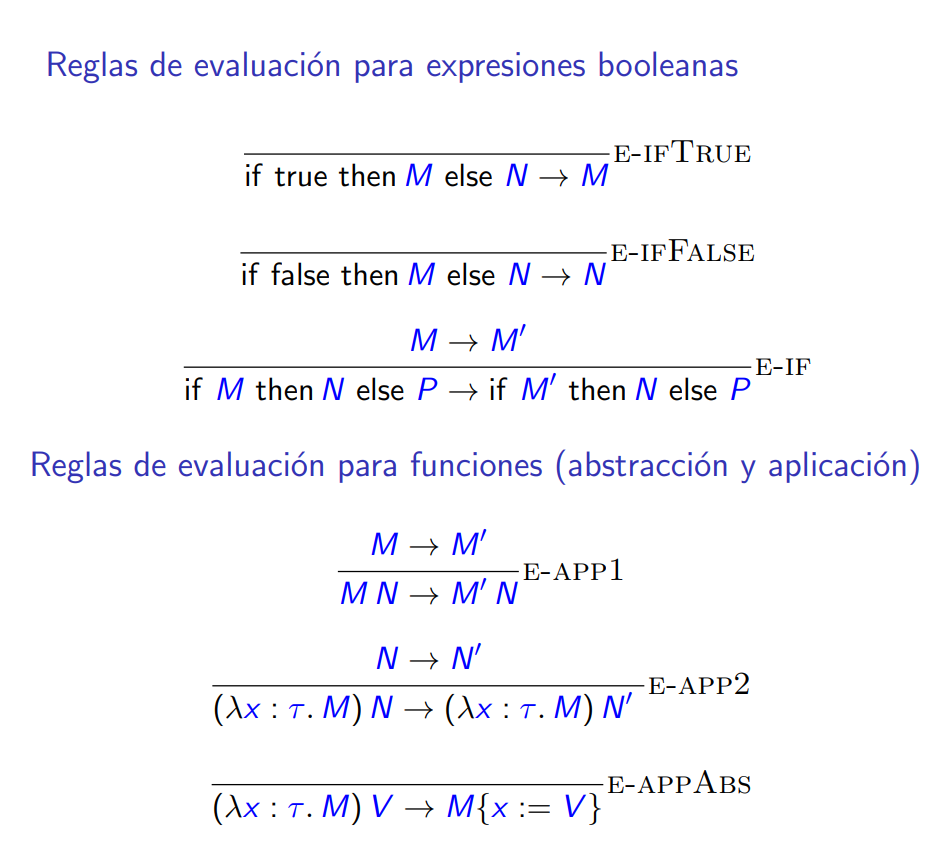
\includegraphics[width=\linewidth]{assets/reglas_operacionales.png}
\end{minipage}\]
\begin{itemize}
    \item 1. Si la guarda es verdadera, entonces el término se reduce a M.
    \item 2. Si la guarda es falsa, entonces el término se reduce a N.
    \item 3. Si el término de la guarda se puede reducir, entonces la reducimos, para obtener el valor (verdadera o falsa). Luego de este paso, aplicamos la regla 1 o la regla 2.
    \item 4. Si el término de M se puede reducir, lo reducimos. Luego le aplicamos a N.
    \item 5. Si el término N se puede reducir, entonces lo reducimos. 
    \item 6. Si el término N es un valor, sustituyo el parámetro de la lambda con el con el valor y lo aplico en el término M.
\end{itemize}
Estas reglas tienen nombres específicos, y se las puede encontrar en la siguiente imagen
\[\begin{minipage}[b]{0.9\textwidth}
    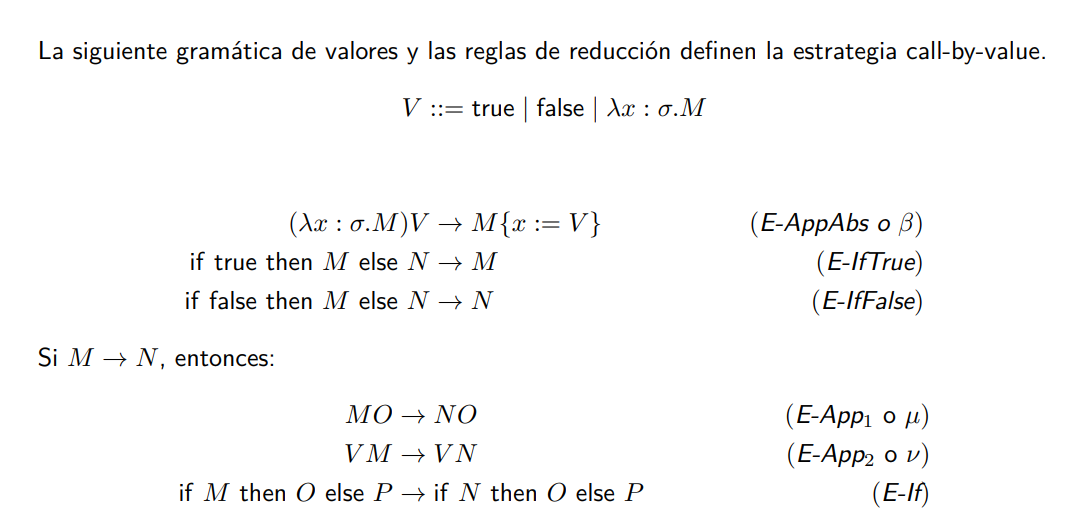
\includegraphics[width=\linewidth]{assets/gramatica_valores_reduccion.png}
\end{minipage}\] 
\subsubsection*{Sustitución}
La operación de sustitución $M\{x:=N\}$ nos devuelve un nuevo término tal que resulta de reemplazar todas las ocurrencias libres de x en M por N. \\
\textbf{Nota}: Se implementa por pattern matching porque es un constructor recursivo. 
\[\begin{minipage}[b]{0.8\textwidth}
    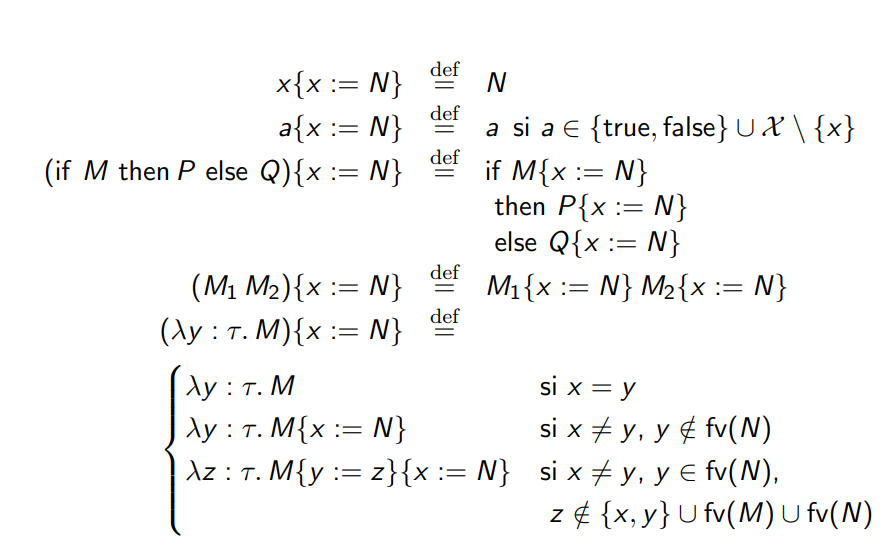
\includegraphics[width=\linewidth]{assets/def_sustitucion.png}
\end{minipage}\] 
\subsection*{Propiedades de la Evaluación}
\subsubsection*{Teorema (Determinismo)}
Si $M \rightarrow N_{1}$ y $M \rightarrow N_{2}$ entonces $N_{1} = N_{2}$ \\
\textbf{En criollo}: No hay más de una forma de reducir algo. 
\subsubsection*{Teorema (Preservación de Tipos o Subject Reduction)}
Si $\Gamma \vdash M : \tau$ y $M \rightarrow N$ entonces $\Gamma \vdash N:\tau$ \\
Si deducimos el tipo $\tau$ para un término sin ejecutar el programa, y luego ejecutamos el programa obteniendo N, entonces el término N tiene el mismo tipo. 
\subsubsection*{Teorema (Progreso)}
Si $\vdash M:\tau$ entonces: 
\begin{itemize}
    \item O bien M es un término cerrado irreducible bien tipado, osea un valor. 
    \item O bien existe un $N$ tal que $M \rightarrow N$
\end{itemize}
\subsubsection*{Teorema (Terminación)}
Si $\vdash M:\tau$ entonces no hay una cadena infinita de pasos: $M \rightarrow M_{1} \rightarrow M_{2} \rightarrow ...$
\subsubsection*{Canonicidad}
\begin{itemize}
    \item Si $\vdash M:bool$ es derivable, entonces la evaluación de M termina y el resultado es true o false.
    \item Si $\vdash M:\tau \rightarrow \sigma$ es derivable, entonces la evaluación de M termina y el resultado es una abstracción. 
\end{itemize}
\subsubsection*{Estado de error}
Cuando el término está en forma normal pero no es un valor.
\subsubsection*{Cantidad de Reglas de Congruencia}
Suele ser una de reducción por cada término, pero es importante recalcar que si un término tiene más de un parámetro (sin variables libres) entonces ese término tiene más de una regla de reducción. \\
A su vez, hay que hacer hincapié en por qué resalté el \textbf{sin variables libres}. Esto es porque los términos que tienen variables libres no se reducen, sino que solamente se sustituyen porque no son términos cerrados. \\
Lo que hay que meterse en la cabeza es que: si no reducimos completamente todo en las reglas de congruencia es: porque o nos falta algo, o se van a sustituir en las reglas de cómputo. TODO debe finalizar siendo un valor. \\
\textbf{Ej.}: Sean $M,N,O :: = \dots \ | \ []_{\sigma} \ | \ M::N \ | \ FOLDR \ M \ BASE \rightarrow N; REC(h,r) \rightarrow O$ \\
¿Qué reglas de Congruencia existen para estos términos? bueno, tenemos aparentemente 3.
\begin{itemize}
    \item Reducir M de M::N
    \item Reducir N de M::N
    \item Reducir M del FOLDR. h NO se reduce porque es un valor (cabeza de la lista) y r tampoco, porque r al ser un caso recursivo tiene variables libres. 
\end{itemize}
\subsubsection*{¿Cuando reducir y cuando no?}
\begin{itemize}
    \item Si tiene variables libres no se reduce. 
    \item Si es un caso condicional, no se reduce, porque de antemano no sabés en qué casos necesitás reducirlo. Por ejemplo, los CASE, IF o FOLDR no se suelen reducir sus términos (sí las guardas), porque no es necesario gastar cómputo en algo que no se sabe si vamos a usar.
\end{itemize}
\subsubsection*{Cantidad de Reglas de Cómputo}
Todos los valores posibles tienen una regla de Cómputo, usualmente, cada valor va a estar asociada a las posibles operaciones de las reglas de Congruencia. \\
Siguiendo el ej. anterior, defina los posibles valores del sistema y dé las reglas de cómputo. \\
Bueno, los posibles valores con listas hay dos: $V::=[]_{\sigma} \ | \ V::V$ \\
¿Qué operaciones deberíamos poder realizar con estos valores?: FOLDR con lista vacía, y FOLDR sin una lista vacía. 
\begin{itemize}
    \item Si el FOLDR tiene lista vacía entonces devuelve simplemente N.
    \item Si el FOLDR NO tiene lista vacía, entonces, debo sustituir las variables h y r con la información para el paso recursivo.
\end{itemize}
\subsubsection*{Árbol Sintático}
Es muy útil hacerlo. \\ 
Véase \hyperref[subsec:arbol_sintatico]{\textbf{\underline{anexo}}} para ver ejemplos para reducir expresiones y verificar si son términos. 
\subsubsection*{Término Bueno}
Decimos que un término es bueno si existe un contexto del que puedo derivarlo. 
\subsubsection*{Término Válido}
Está atado a como está sintácticamente formado. Es importante que solo tengan tipos válidos.
\begin{itemize}
    \item $x M$: No es válido. No podemos usar genéricos como M.
    \item $\lambda x:Bool$: No es válido. Las funciones toman algo y devuelven algo. Esta lambda no es $\tau \rightarrow \tau$.
    \item $\lambda x.x$: No es válido. No sabemos el tipo de x.
    \item if $x$ then $\lambda x:Bool x$: No es válido, los condicionales tienen una rama else.
    \item $\lambda x: Bool \rightarrow Bool . xy \ \lambda y: Bool . x$
    \begin{itemize}
        \item Si colocamos los paréntesis de la asociación queda así: $((\lambda x: Bool \rightarrow Bool . x \textbf{y}) \ (\lambda y: Bool . \textbf{x}))$
        \item Por un lado se resuelve $(\lambda x: Bool \rightarrow Bool . xy)$ y por otro $(\lambda y: Bool . x)$.
        \item Finalmente, cuando reduce, se realiza la aplicación. En negrita, están marcadas las variables libres.
        \item Este término es válido.
    \end{itemize}
    \item $\lambda y:\sigma . y$: No es válido, no existe el tipo $\sigma$. Solo existe $Bool \ | \ \tau \implies \tau$
    \item $xy \ \lambda x: Bool \rightarrow Bool . xy$
    \begin{itemize}
        \item Asociemos hacia la izquierda entonces queda $(xy) \ (\lambda x: Bool \rightarrow Bool . xy)$
        \item Cada lado se resuelve por separado y luego se componen.
    \end{itemize}
\end{itemize}
Para ver ejemplos de esto utilizando árboles sintáticos véase \hyperref[subsec:arbol_sintatico]{\textbf{\underline{anexo}}}
\subsubsection*{Tipando operaciones}
\[\begin{minipage}[b]{0.8\textwidth}
    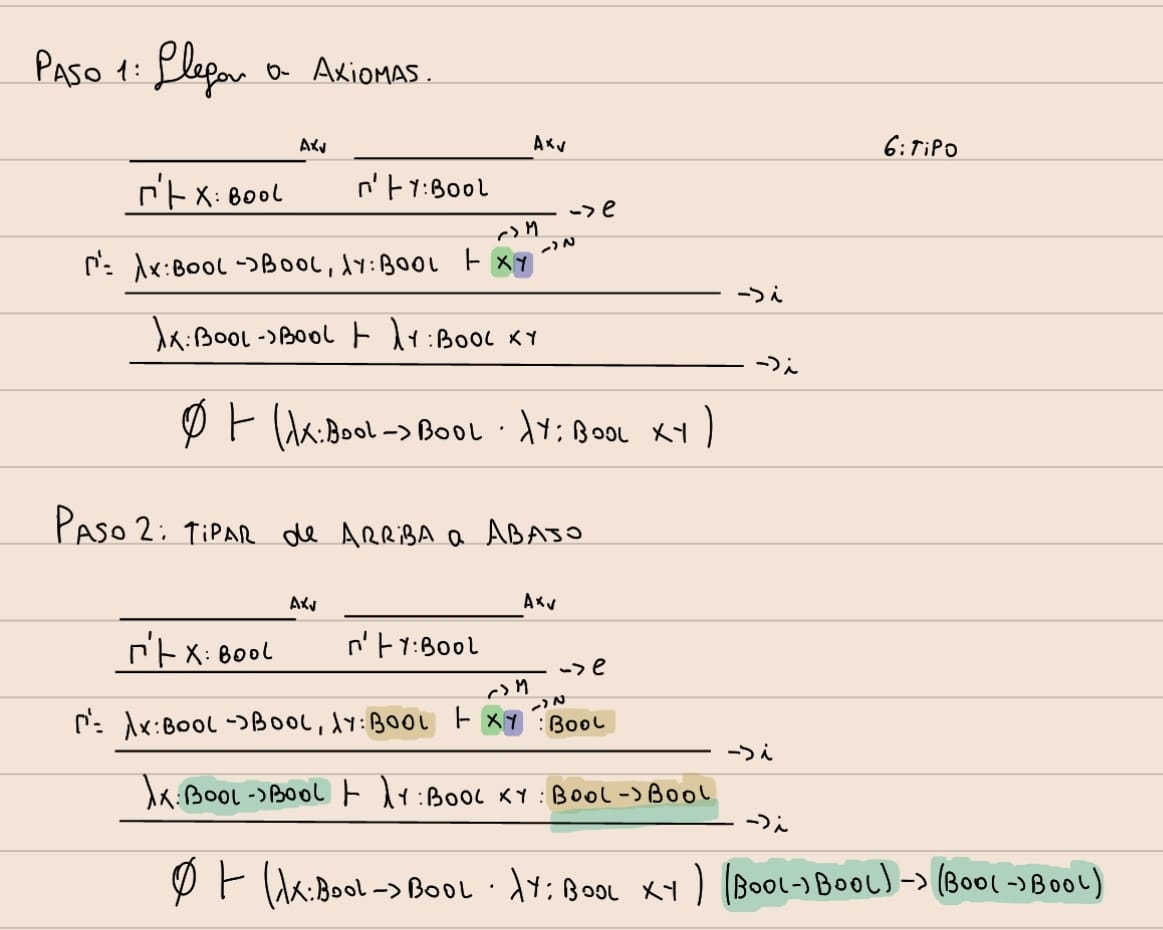
\includegraphics[width=\linewidth]{assets/tipado_operaciones.jpg}
\end{minipage}\]
\[\begin{minipage}[b]{0.8\textwidth}
    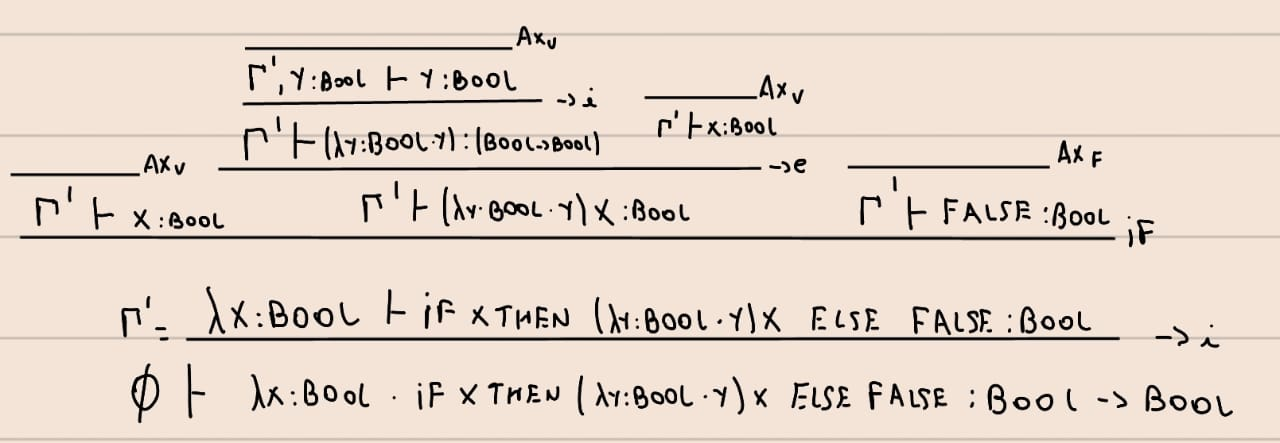
\includegraphics[width=\linewidth]{assets/tipado_condicional.jpg}
\end{minipage}\]
\subsubsection*{Aplicando Clases de Equivalencia}
Recordemos que las variables ligadas, en cualquier lenguaje de programación serían como el parámetro de una función y da igual que nombre le pongamos. Lo importante es NO tener dos parámetros con el mismo nombre.
\[\begin{minipage}[b]{0.9\textwidth}
    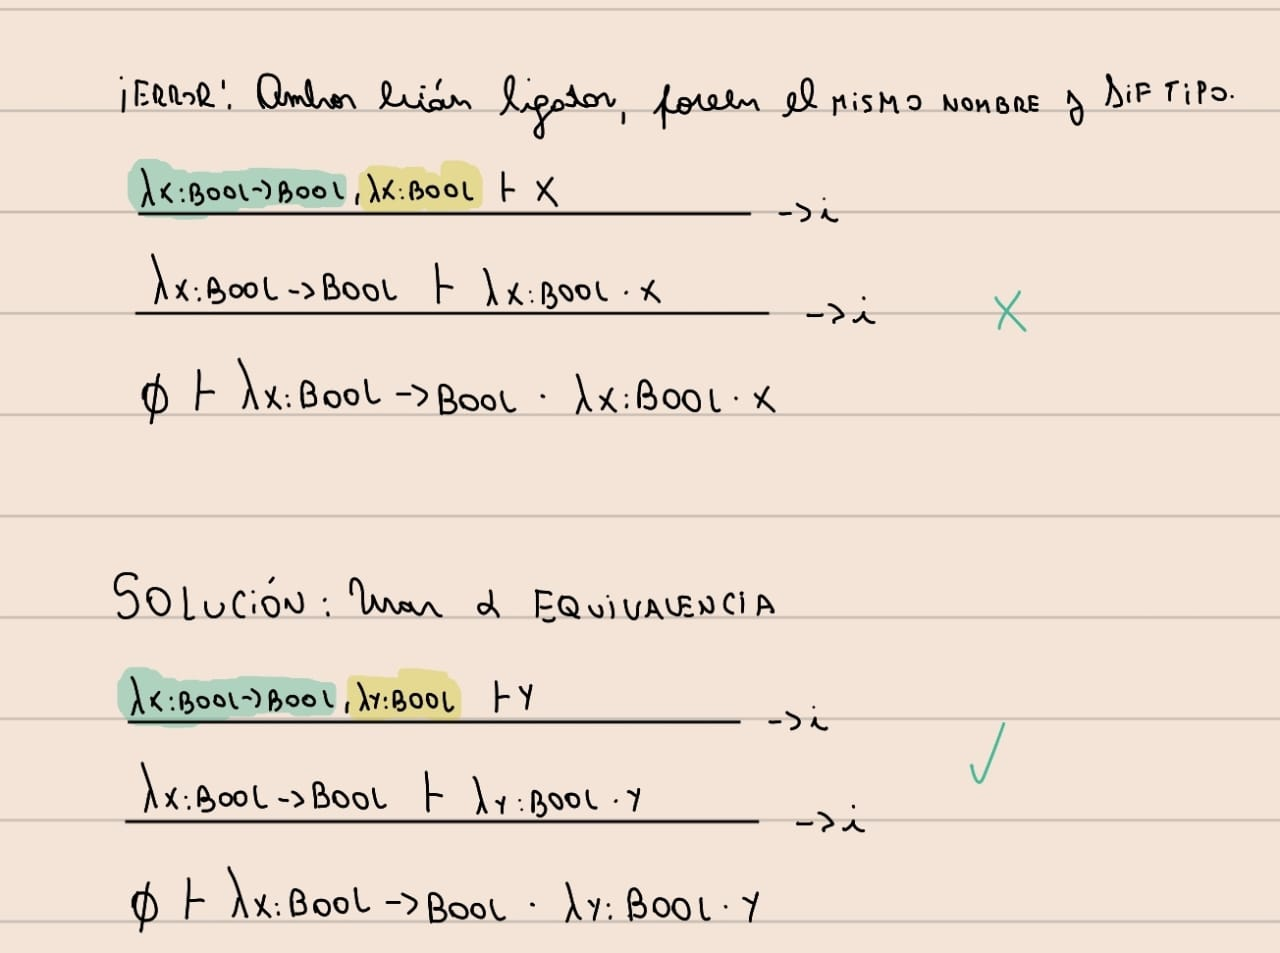
\includegraphics[width=\linewidth]{assets/alfa_reduccion.jpg}
\end{minipage}\]
\textbf{Nota}: Al igual que en un lenguaje de programación da igual a qué variable ligada le cambiemos su nombre.
\subsubsection*{Reglas de Tipado vs Reglas de Semántica}
\textbf{1}. En las Reglas de Tipado \textbf{existe} el contexto mientras que en las Reglas de Semántica \textbf{no existe}. \\
La excepción de usar un contexto en las reglas de semántica se da cuando tenemos alguna especie de guarda o un caso donde tenemos que devolver cosas de algún tipo específico, pero sin contexto no tenemos esa información. \\
\sd{\emptyset \vdash V_{1}:\sigma}{FROM \ V_{1} \ UNTIL_{x} N \ BY \ V_{2} \rightarrow IF \ N \{x:=V_{1}\} \ THEN \ []_{\sigma} \ ELSE \ V_{1}::(FROM \ V_{2}V_{1} \ UNTIL_{x} \ N \ BY \ V_{2})}{} \\
En este ejemplo podemos ver que como estamos en un lenguaje con \textbf{tipado estricto}, necesitamos que tanto el THEN como el ELSE devuelvan el mismo tipo. Entonces no podemos devolver una lista vacía sin especificar el tipo de sus elementos.  \\
\textbf{2}. En las Reglas de Semántica no se coloca el tipo de retorno en cada una de las reglas.  
\subsubsection*{Extensión con Números Naturales}
Sintaxis:
\[\begin{minipage}[b]{0.8\textwidth}
    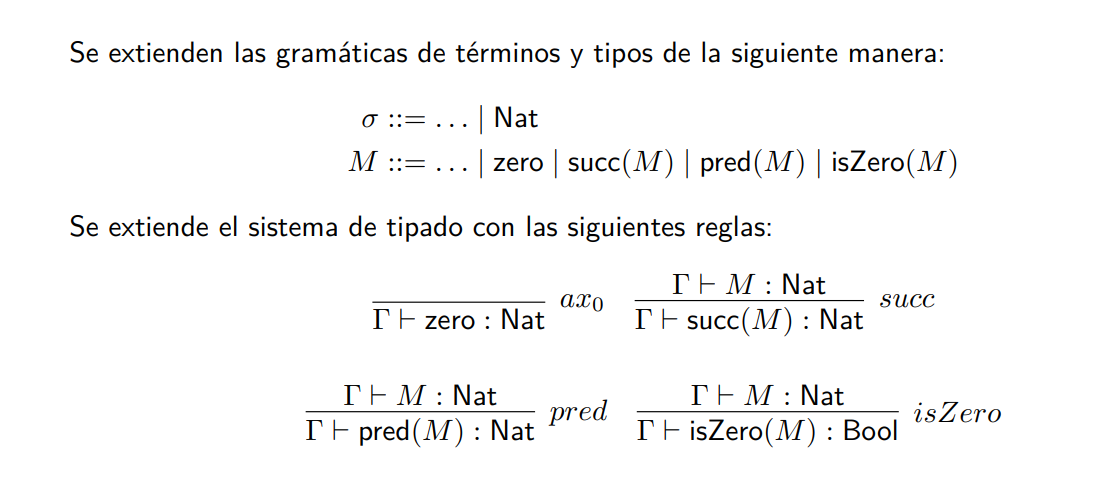
\includegraphics[width=\linewidth]{assets/extension_naturales.png}
\end{minipage}\]
Semántica:
\[\begin{minipage}[b]{0.8\textwidth}
    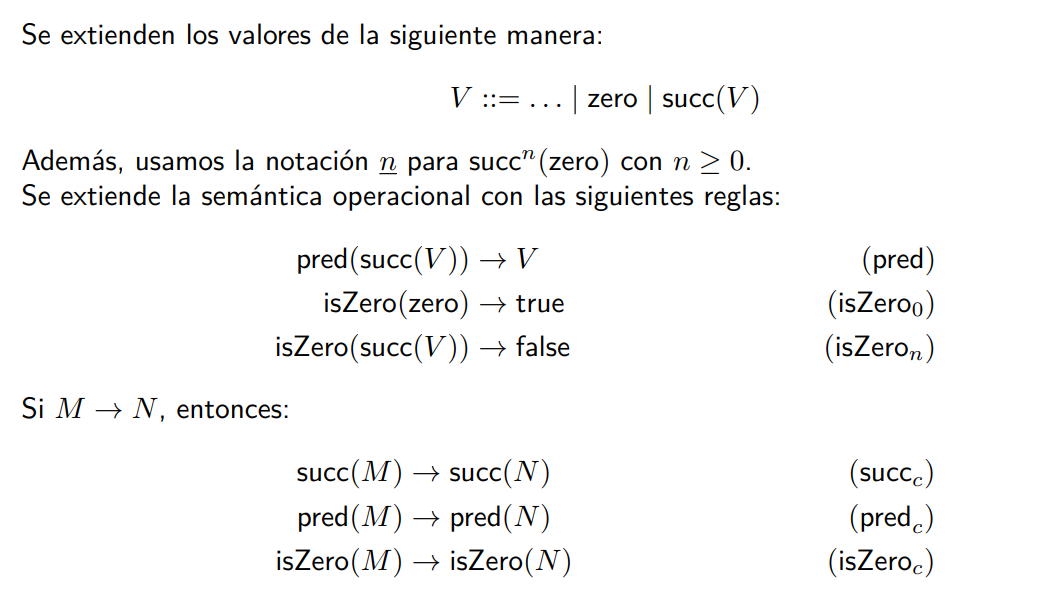
\includegraphics[width=\linewidth]{assets/extension_naturales_semantica.png}
\end{minipage}\]
\textbf{Ultra Importante}: Cada vez que extendmos tipos o sintaxis hay que chequear que siga valiendo el progreso, el determinismo y la preservación de tipos. \\
\textbf{¿Es segura esta extensión?}: No, porque con estas reglas se rompe el progreso pues pred(0) es forma normal pero no es un valor válido. \\
Si quisieramos que siga valiendo el progreso podemos extender la semántica y agregar un caso \textbf{$pred(zero) \rightarrow zero$ ($pred_{0}$)}
\subsubsection{Macros}
\[\begin{minipage}[b]{0.8\textwidth}
    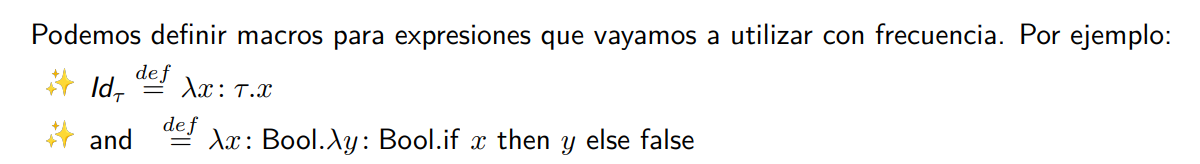
\includegraphics[width=\linewidth]{assets/macros.png}
\end{minipage}\]
\subsubsection{Agregando Reglas para las Abstracciones}
\[\begin{minipage}[b]{0.8\textwidth}
    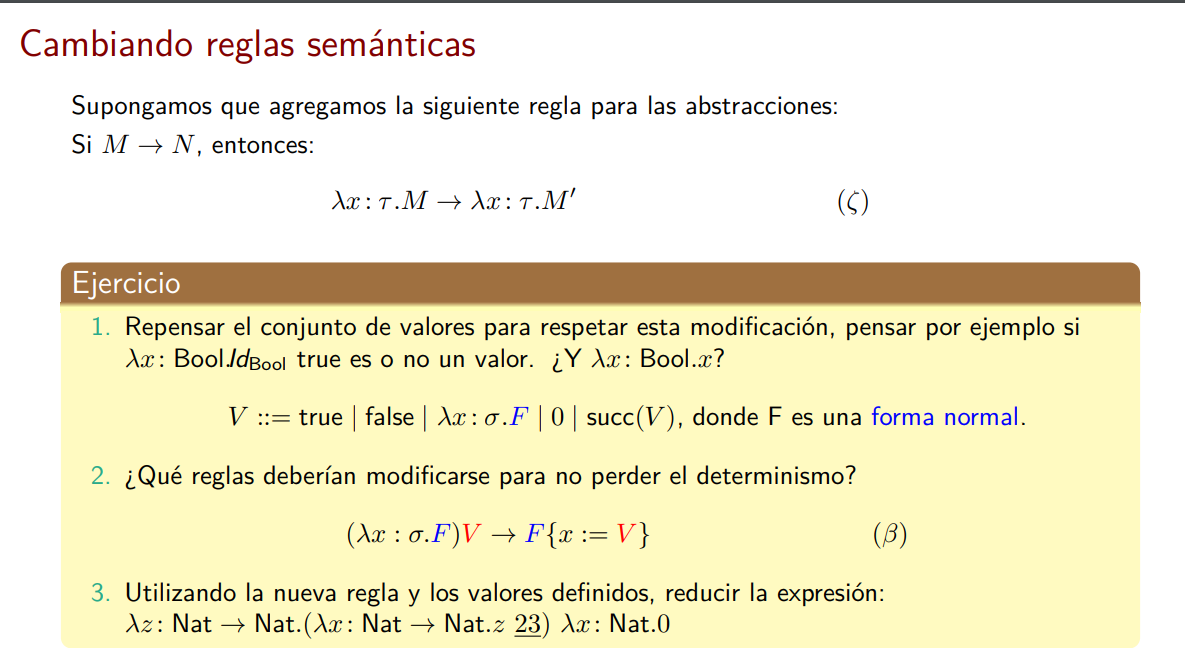
\includegraphics[width=\linewidth]{assets/forma_normal.png}
\end{minipage}\]
(No entendí qué caso es el conflictivo si tuvimos que cambiar de $\lambda x: \sigma . M$ a $\lambda x:\sigma . F$) ¿qué no podíamos hacer antes? \\
Entiendo que diciendo que tengas $\lambda x:\sigma . F$ estas diciendo que si le metés un input tenés que garantizar que lo que tenga la lambda adentro \textbf{ya sea una forma normal} y sabés que el proceso va a terminar bien. \\
Si usás $\lambda x: \sigma . M$ tenés el problema de que si le ponés cualquier cosa a M podés llegar a algo que no es reducible y capaz se cuelga? 
\subsection*{Sistema de Tipos para el Cálculo Lambda}
\textbf{Aclaración Importante}: En deducción natural hablabamos de $\tau, \sigma$ como hipótesis o proposiciones. Acá en cálculo lambda, esos son tipos. \\
Ej.: $\tau \rightarrow \sigma$ era una conclusión en deducción natural, acá es el tipo de una lambda. \\
Entonces ahora sí, veamos el sistema de tipos para el cálculo Lambda omitiendo los booleanos porque son exactamente igual que en deducción natural. \\
\sd{\Gamma, x:\tau \vdash M:\sigma}{\Gamma \vdash \lambda x: \tau.M: \tau \rightarrow \sigma}{T-ABS ($\rightarrow i$)}
\sd{}{\Gamma, x: \tau \vdash x:\tau}{T-VAR (ax)}
\sd{\Gamma \vdash M:\tau \rightarrow \sigma r \vdash N:\tau}{\Gamma \vdash MN:\tau}{T-APP ($\rightarrow$ e)}
\subsubsection{Lógica Combinatoria}
Es una variante del calculo $\lambda$. \\
Si a $\sigma \rightarrow \tau$ lo leemos como $\sigma \implies \tau$ luego, la regla de tipadod e aplicación de una función es la regla Modus Ponens. \\
\subsection*{Pruebas y Programas}
En la \textbf{Deducción Natural} hablamos en base a proposiciones, en cálculo lambda, las proposiciones son tipos. \\
En la \textbf{Deducción Natural} hablamos en base a pruebas, en cálculo lambda, las pruebas son términos. 
\subsubsection{Juicios Derivables}
Un juicio $\vdash \tau$ es derivable sí y solo sí, el tipo $\tau$ está habitado, es decir, existe algun camino que nos lleva a demostrar $\tau$. \\
Como también podemos probar estas cosas en deducción natural, lo hacemos también en cálculo lambda. \\
\[\begin{minipage}[b]{0.8\textwidth}
    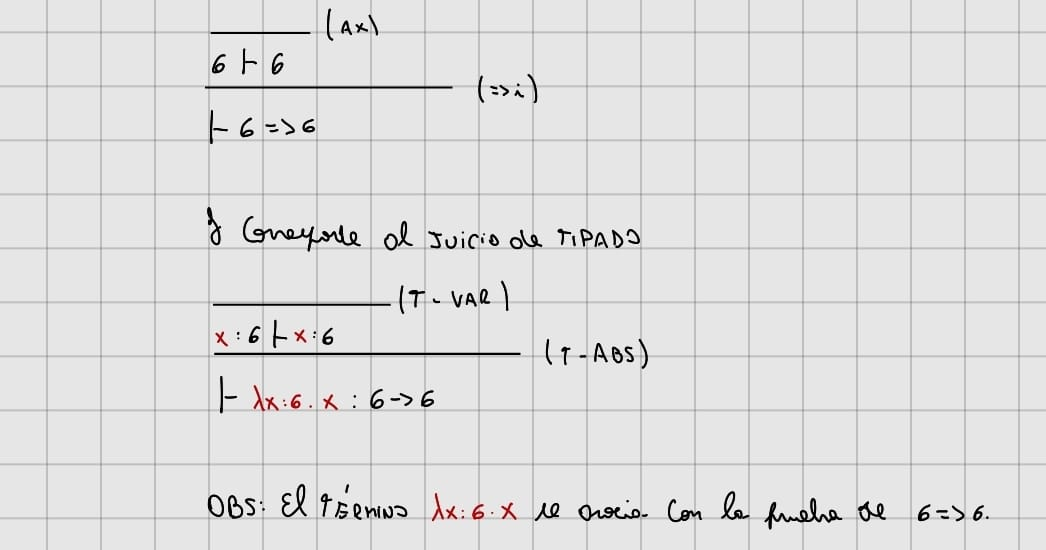
\includegraphics[width=\linewidth]{assets/juicio_tipado_lambda.jpg}
\end{minipage}\]
\textbf{Importante}: Como esto son fórmulas, puede haber muchas pruebas distintas para una misma fórmula. Mirá esta forma de probar lo mismo de antes pero más complicado.
\[\begin{minipage}[b]{0.8\textwidth}
    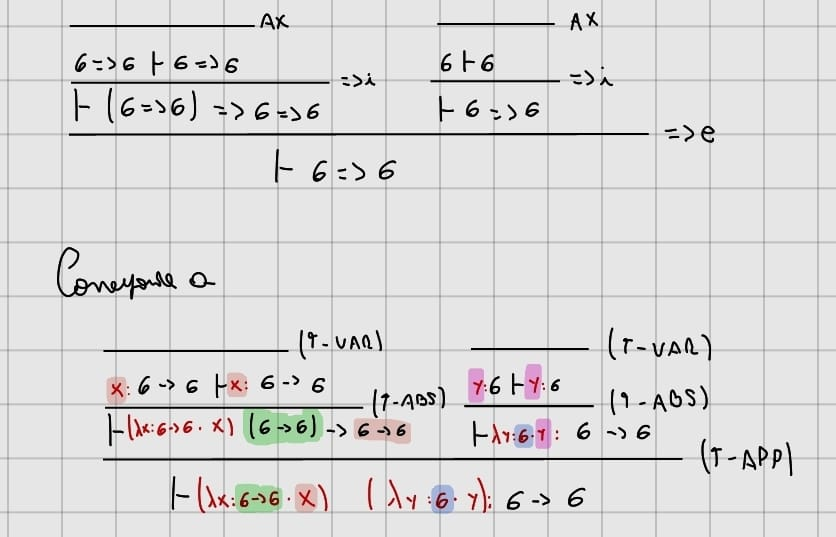
\includegraphics[width=\linewidth]{assets/juicio_tipado_lambda_2.jpg}
\end{minipage}\]
\subsubsection{Simplificación de Pruebas}
Corte: Un corte es un lema que probamos a pesar que \textbf{no es una subfórmula de la afirmación final}. Es decir, no es algo que queramos demostrar en la conclusión pero nos ayuda a seguir adelante. \\
Se caracteriza por tener pasos como $\implies_{i}$ y luego $\implies_{e}$ o también, $\land_{i}$ y $\land e_{1}$ o $\land e_{2}$. \\
Básicamente cuando veas una introducción y una eliminación, ahí estás haciendo un corte. \\
La variable que hacés aparecer aparte es el corte. \\
En la computación, un paso de reducción $\beta$ (E-APP ABS) se corresponde con una eliminación de corte. 
\subsubsection{Prueba en Forma Normal}
Es aquella prueba que no posee ningún tipo de corte. 
\subsubsection{Normalización de Pruebas}
Se realiza mediante la eliminación de cortes, es decir, tratar de quitar esos cortes para llevarlo a forma normal. 
\subsubsection{Conjunción (Producto) en Lambda}
\[\begin{minipage}[b]{0.6\textwidth}
    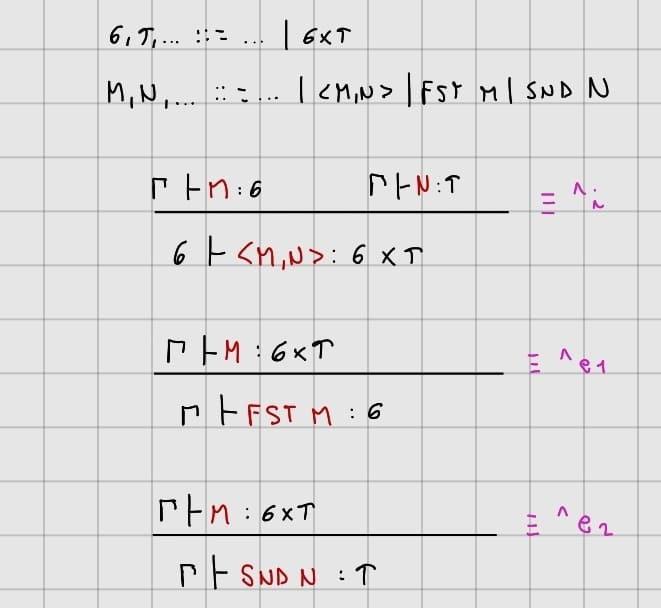
\includegraphics[width=\linewidth]{assets/conjuncion_lambda.jpg}
\end{minipage}\]
Veamos ahora como hacer reducciones con productos. 
\[\begin{minipage}[b]{0.6\textwidth}
    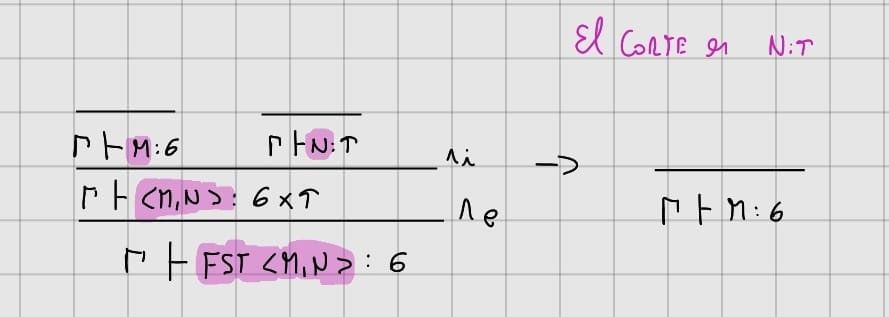
\includegraphics[width=\linewidth]{assets/producto_corte.jpg}
\end{minipage}\]
Nótese que la idea desde un primer momento era quedarse con M $\sigma$. Por lo tanto, el corte es añadir $\tau$.
\subsubsection{Disyunción (Suma) en Lambda} 
El corte característico acá es $\lor_{e}$ y luego $\lor_{i}$ mirando desde abajo hacia arriba. 
\[\begin{minipage}[b]{0.74\textwidth}
    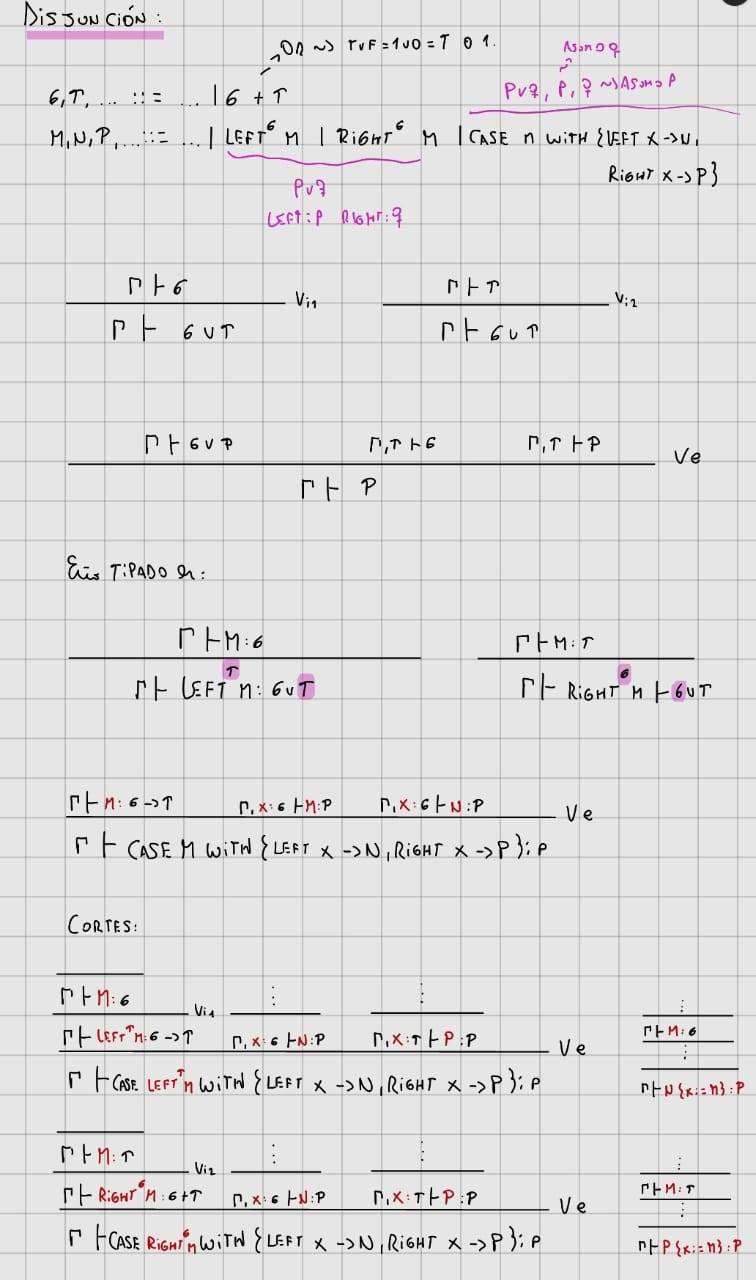
\includegraphics[width=\linewidth]{assets/disyuncion.jpg}
\end{minipage}\]
\subsubsection{Absurdo}
No existe \textbf{ningún constructor} para el tipo $\bot$ (vacío). 
\[\begin{minipage}[b]{0.7\textwidth}
    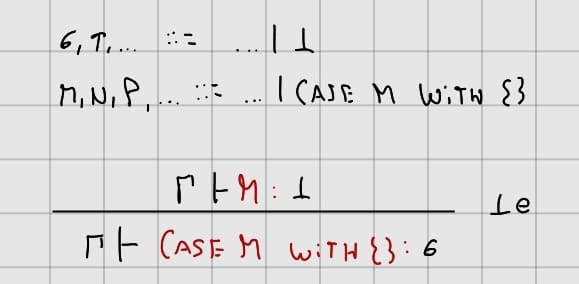
\includegraphics[width=\linewidth]{assets/absurdo_lambda.jpg}
\end{minipage}\]
\subsection*{Correspondencia de Curry-Howard}
$A_{1},...A_{n} \vdash \sigma$ es derivable en NJ (Logica Intusionista) si $\exists$ término $M$ donde $Fv(M) \subseteq \{x_{1}, ..., x_{n}\}$ tal que $x_{1}:A_{1}, ..., x_{n}:A_{n} \vdash M:\sigma$ \\
\textbf{En criollo}: Si en Cálculo Lambda tenes términos $x_{1}, ..., x_{n}$ que correspondan a $A_{1}, ..., A_{n}$ uno a uno entonces, lo podés considerar como válido. \\
Ej.: $P, Q \vdash P \land Q \equiv x:P, y:Q \vdash <x, y>: P \land Q$ donde 
\begin{itemize}
    \item $A_{1} = P \ A_{2} = Q$
    \item $x_{1}:P$ es decir, $x_{1}:A_{1}$
    \item $x_{2}:Q$ es decir, $x_{2}:A_{2}$
    \item $\sigma = P \land Q$ pero en cálculo lambda, nuestro término M, es de tipo sigma. $<x,y>:P \land Q$
\end{itemize}
\subsubsection{Corolario de Logica Intusionista}
$\nvdash \bot$: No puedo concluir que hay contradicción, lo que sugiere que mis premisas son consistentes. 
\subsubsection{Codificación de la Negación}
$\neg \sigma \equiv \sigma \rightarrow \bot$ \\
\textbf{Nota}: $\neg_{i} \equiv \implies i $ y $\neg_{e} \equiv \implies e$ \\
\subsubsection{Tipo Unit}
También conocida como Fórmula T, es una fórmula válida que siempre es verdadera y es un tipo algebraico con un único constructor T. \\
En el cálculo $\lambda$ extendemos la sintaxis con el tipo T que tiene un único elemento. 
\[\begin{minipage}[b]{0.3\textwidth}
    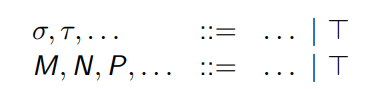
\includegraphics[width=\linewidth]{assets/extension_lambda_t.png}
\end{minipage}\]
Consideramos a la Logica Intusionista extendida con la siguiente regla \\
\sd{}{\Gamma \vdash T}{$T_{i}$} 
Y tiene la siguiente regla de tipado en Cálculo $\lambda$ \\
\sd{}{\Gamma \vdash T:T}{T-UNIT} 
\subsubsection{Recursión}
Se utiliza el operador fix: $M ::= ... \ | \ fix \ M$\\
No se precisa ningún tipo nuevo pero sí una regla de tipado. \\
\sd{\Gamma \vdash M : \sigma \rightarrow \sigma}{\Gamma \vdash fix \ M : \sigma}{T-FIX} \\
También extendemos la semántica para poder ir resolviendo las operaciones. 
\[\begin{minipage}[b]{0.6\textwidth}
    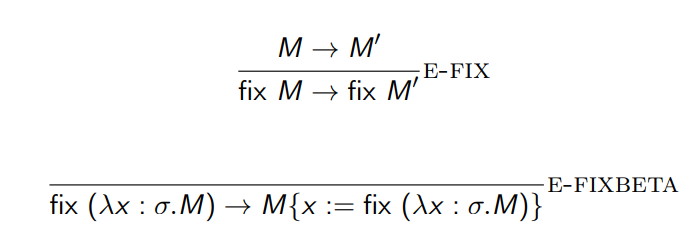
\includegraphics[width=\linewidth]{assets/fix_recursion.png}
\end{minipage}\]
Gracias a fix ahora podemos definir funciones parciales $fix \ (\lambda x: \sigma . x)$ donde $\vdash \ fix \ (\lambda x:\sigma.x):\sigma$ para cualquier $\sigma$. En particular, vale para $\sigma = \bot$ \\
\textbf{Importante}: No podemos extender la Lógica Intusionista (NJ) con un operador fix pues la lógica sería inconsistente. Ej.: $\vdash \bot$ sería derivable.
\section*{Inferencia de Tipos}
\textbf{Términos \textcolor{red}{sin} anotaciones de tipos}: U :: = x | $\textcolor{red}{\lambda x.U}$ | U U | True | False | if U then U else U \\
\textbf{Términos \textcolor{blue}{con} anotaciones de tipos}: U :: = x | $\textcolor{blue}{\lambda x.M}$ | M M | True | False | if U then U else U
\subsection*{erase(M)}
Es el término sin anotaciones de tipos que resulta de borrarlos del término M. El resultado es U. \\
Ej.: $erase((\lambda x:Bool . x) \ True) = ((\lambda x . x) \ True)$ \\
Esto nos quiere decir que, si tenemos un término M es fácil conseguir U pero no al revés. 
\subsection*{¿Cuándo podemos tipar un término U?}
Un término U sin anotaciones de tipos es tipable sí y solo sí existen: 
\begin{itemize}
    \item Un contexto de tipado $\Gamma$
    \item Un término con anotaciones de tipos M 
    \item Un tipo $\tau$
    tales que erase(M) = U y $\Gamma \vdash M:\tau$
\end{itemize}
Entonces, el problema de \textbf{inferencia de tipos} consiste en: 
\begin{itemize}
    \item Dado un término U determinar si es tipable.
    \item En caso de que U sea tipable, entonces
    \begin{itemize}
        \item Hallar un contexto $\Gamma$, un término $M$ y un tipo $\tau$ tales que cuando hagamos erase(M) = U y $\Gamma \vdash M:\tau$
    \end{itemize}
\end{itemize}
\textbf{En criollo}: Si tengo un U, entonces buscate un M, que tenga contexto, un $\tau$ y que si le mando ese M me da U. \\
Ej.: $\lambda x . x$ es la función identidad. ¿Cómo podemos tiparla?. De antemano, x podría ser cualquier cosa, una función, un valor, lo que realmente quiera. \\
Entonces para poder tiparla, necesitamos de antemano, saber en el contexto de qué tipo es x, por lo tanto, podemos decir que $\Gamma \vdash \{x: \alpha\}$. \\
Ya tenemos entonces $\Gamma$ y $U$. Nos falta conseguir $\tau$ que sería lo que nos falta para poder concluir $\Gamma \vdash M:\tau$. Como es una Lambda que recibe un x, y devuelve un x, entonces el tipo es $\tau:\alpha \rightarrow \alpha$. \\
Entonces, armamos el término M: $\lambda(x:\alpha) . x$ y podemos chequear ambas condiciones.
\begin{itemize}
    \item erase($\lambda(x:\alpha) . x$) = $\lambda x . x$ y esto es verdadero.
    \item $\Gamma \vdash (\lambda(x:\alpha) . x):\alpha \rightarrow \alpha$
\end{itemize}

\sd{\Gamma ,x:\alpha \vdash x:\alpha}{\Gamma \vdash (\lambda(x:\alpha) . x):\alpha \rightarrow \alpha}{T-ABS} y es justamente lo que queríamos derivar. \\
\textbf{Importante}: Solo tipo en M si $\exists$ una lambda. Ej.: $U = x \ True \equiv M = x \ True $ pues no existe ninguna lambda en U. 
\subsection*{Incorporando incógnitas a los tipos}
El algoritmo de inferencia de tipos se basa en manipular tipos \textbf{parcialmente conocidos}. \\
Ej.: $x \ True$, ¿cómo podemos tiparlo?. Bueno, recordemos que asociamos a la izquierda, por lo tanto sería algo así: $x(True)$ por lo tanto, x debería de ser una función que recibe obligatoriamente un booleano y devuelve un tipo desconocido. Ese tipo desconocido lo denotamos con una variable. \\
Por lo tanto, el tipo sería: (x: $Bool \rightarrow X_{1}$) \\
Ej. 2: $(X_{1} \rightarrow X_{1}) \stackrel{?}{=} ((Bool \rightarrow Bool) \rightarrow X_{2})$. \\
En criollo lo que nos pide es: ¿cómo tiene que ser X1 y X2 para que ambos lados se verifiquen? bueno, si vemos la ecuación izquierda antes de $\rightarrow$ tiene $Bool \rightarrow Bool$ entonces no queda otra que $X_{1} = Bool \rightarrow Bool$ 
Así mismo, entonces, del lado izquierdo nos queda $Bool \rightarrow Bool \rightarrow Bool \rightarrow Bool = (Bool \rightarrow Bool) X_{2}$ entonces la única forma que tiene $X_{2}$ es $Bool \rightarrow Bool$. \\
Por lo tanto, $X_{1}: Bool \rightarrow Bool$ y $X_{2}: Bool \rightarrow Bool$ \\
Ej. 3: if xy then y else true \\
La estrategia en los condicionales, o lugares donde hay ramas es la siguiente: \textbf{considerar y tipar cada rama por separado, luego se hace puesta en común}. \\
Entonces, en este caso tenemos que tipar tres ramas, una incógnita por cada variable: 
\begin{itemize}
    \item xy: $\Gamma_{c} = \{x: X_{1} \rightarrow X_{2}, y: X_{1}\}$
    \item y: $\Gamma_{t} = \{t: X_{3}\}$
    \item true: $\Gamma_{e} = \emptyset$
\end{itemize}
Entonces ahora planteamos un sistema de ecuaciones 
\(
\begin{cases} 
    X_{3} \stackrel{?}{=} Bool \\
    X_{1} \stackrel{?}{=} X_{3} \\
    X_{2} \stackrel{?}{=} Bool
\end{cases}
\) \\
Sustituimos ahora las incógnitas por los tipos y nos queda $X_{1} = Bool, X_{2} = Bool, X_{3} = Bool$. \\
Resolver ecuaciones del tipo $X_{1} \stackrel{?}{=}X_{2} \rightarrow X_{3}$ se llama UNIFICACIÓN. Reemplazando las variables deberíamos llegar a una igualdad. 
\subsection*{Unificación}
Es el problema de resolver sistemas de ecuaciones entre tipos con incógnitas. Es muy importante pues luego lo usamos para dar un algoritmo de inferencia de tipos. \\
Tenemos conjuntos finitos de constructores de tipos 
\begin{itemize}
    \item Tipos constantes (no tienen parámetros): Bool, Int, ...
    \item Constructores Unarios (reciben un parámetro): (List $\bullet$), (Maybe $\bullet$), ...
    \item Constructores Binarios (reciben dos parámetros): $(\bullet \rightarrow \bullet)$, ($\bullet \times \bullet$), ($Either \bullet \bullet$)
\end{itemize}
Los \textbf{tipos} se forman usando incógnitas y constructores: $\tau ::= X_{n} \ | \ C(\tau_{1}, \dots, \tau_{n})$ \\
Antes de definir formalmente la Unificación, primero veamos la Sustitución, que es una de las herramientas que vamos a usar.
\subsubsection*{Sustitución}
Es una función que a cada incógnita le asocia un tipo. \\
Notamos: $\{T_{1} \stackrel{?}{=} \sigma_{1}, \dots, T_{k}\stackrel{?}{=}\sigma_{k}\}$ a la sustitución S tal que $S(T_{1}) = S(\sigma_{1}) \land \dots \land S(T_{k}) = S(\sigma_{k})$ \\
Si $\sigma$ es un tipo, escribimos $S(\sigma)$ para que cada incógnita de $\sigma$ sea reemplazada por lo que haya sido definido en S. \\

Ej.: Si $S = \{X_{1} := Bool, X_{3} := (X_{2} \rightarrow X_{2})\}$ entonces S(($X_{1} \rightarrow Bool) \rightarrow X_{3}$) = $(Bool \rightarrow Bool) \rightarrow (X_{2} \rightarrow X_{2})$ 
\subsubsection*{Unificación}
Un problema de unificación es un conjunto finito E de ecuaciones entre tipos que pueden involucrar incógnitas. \\
Un \textbf{unificador} para E es una sustitución \textbf{S} tal que 
\begin{itemize}
    \item $S(\tau_{1}) = S(\sigma_{1})$
    \item ... 
    \item $S(\tau_{n}) = S(\sigma_{n})$
\end{itemize}
Ej.: $\{X_{1} \stackrel{?}{=} X_{2}\}$ mientras que sea una igualdad, se puede decir cualquier cosa de $X_{1}$ y $X_{2}$. Todas serán solución pero si la solución tiene menos variables para solucionar el problema, es más general. 
\subsubsection*{Sustitución más general}
Una sustitución \textbf{$S_{A}$} es \textbf{más general} que una sustitución \textbf{$S_{B}$} si existe una sustitución \textbf{$S_{C}$} tal que: $S_{B} = S_{C} \circ S_{A} $ \\
\textbf{En Criollo}: Si $S_{B}$ nace de $S_{A}$ particularmente, entonces $S_{A}$ es más general.
\subsection*{Algoritmo de unificación Martelli-Montanari (M-M) y la Corrección del Algoritmo}
Consiste en aplicar secuencialmente un conjunto de reglas las cuales hay dos chances: o falla, o sigue adelante reemplazando. Este algoritmo siempre termina para cualquier problema de unificación E.
\begin{itemize}
    \item Mientras que $E \neq \emptyset$ se aplica sucesivamente alguna de las reglas.
    \item La regla puede resultar en una falla (si E no tiene solución)
    \item De lo contrario, la regla es de la forma $E \rightarrow_{s} E'$ y al aplicarlo sucesivamente, si no hay falla, el algoritmo llega a $\emptyset$: 
    \begin{itemize}
        \item $E = E_{0} \rightarrow_{S_{1}} \ E_{1} \rightarrow_{S_{2}} E_{2} \dots \rightarrow_{S_{n}} E_{n} = \emptyset$
        $S = S_{n} \circ S_{n-1} \dots \circ S_{2} \circ S_{1}$ es un unificador para E, es el más general posible y lo denotamos mgu(E).
    \end{itemize}
\end{itemize}
\subsubsection*{Reglas del Algoritmo (M-M)}
\[\begin{minipage}[b]{0.7\textwidth}
    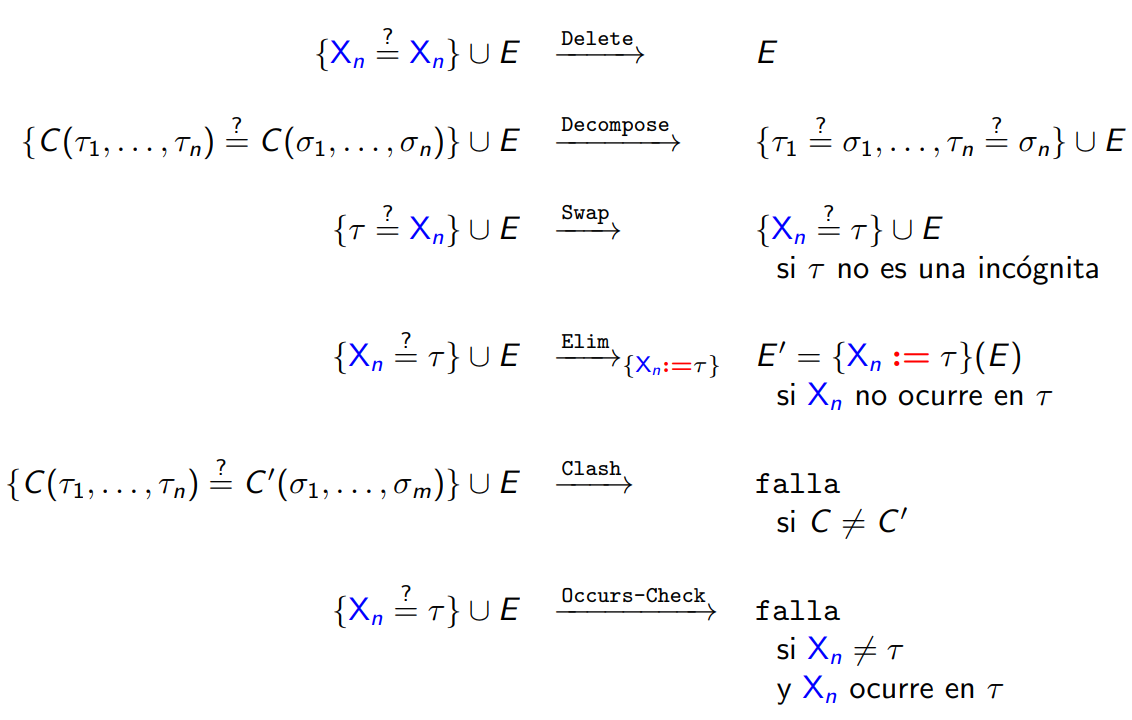
\includegraphics[width=\linewidth]{assets/algoritmo_m_m.png}
\end{minipage}\]
¿Por qué los condicionales en las reglas?
\begin{itemize}
    \item Swap: $\tau$ no debe ser una variable. Debe ser un valor porque sino entramos en un loop infinito de hacer referencia a sí mismo. Ej.: $4 = x \equiv x = 4 $ pero x = y $\neq$ y = x NO es lo mismo porque NO son valores.
    \item Elim: No podemos reemplazar un término que depende de sí mismo y reducirlo. Ej.: $X_{1} = X_{1} \rightarrow Bool$ no tiene sentido sustituir en este caso porque vamos a estar en prácticamente un loop infinito. 
    \item Clash: Si no tienen la misma cantidad de elementos falla.
    \item Occurs-Check: Solo podemos unificar si la incógnita no aparece en $\tau$. Ej.: $X_{1} = X_{1} \rightarrow Bool$ falla pero $X_{1} = Int$ funciona. 
\end{itemize}
La regla Decompose es muy útil para separar funciones. La Delete la hacemos cuando nos queda una igualdad trivial. La Elim la usamos dejando todo menos la igualdad que queremos quitar.
\[\begin{minipage}[b]{0.9\textwidth}
    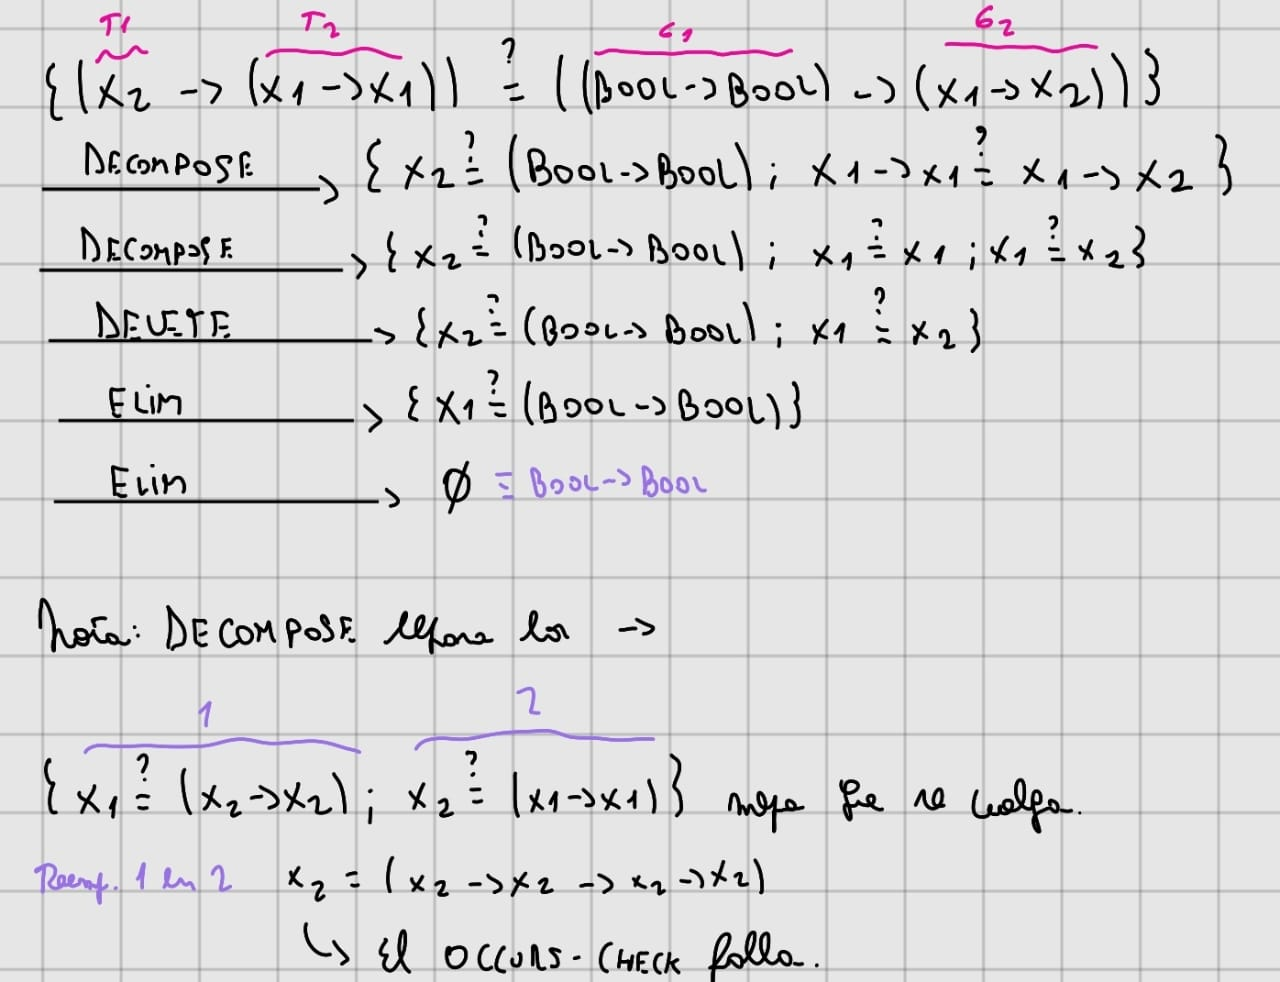
\includegraphics[width=\linewidth]{assets/alg_m_m.jpg}
\end{minipage}\]
\textbf{Nota}: El MGU del primer ejercicio sería lo mínimo indispensable para cumplir la igualdad. En este caso sería $X_{1}: Bool \rightarrow Bool, \ X_{2}: Bool \rightarrow Bool$ \\
\textbf{Importante}. El algoritmo de simplificación \textbf{no siempre} devuelve el mismo resultado si existe una solución.
\subsection*{Algoritmo W (Inferencia de Tipos)}
La idea es siempre empezar haciendo las reglas de tipado. La regla de tipado deriva el algoritmo de inferencia. \\
Al igual que el Algoritmo M-M hay dos opciones
\begin{itemize}
    \item Puede fallar si U no es tipable.
    \item Puede tener éxito y si lo tiene devuelve una tripla $(\Gamma, M, \tau)$ donde $erase(M) = U$ y $\Gamma \vdash M:\tau$ ¡sí! es lo mismo que vimos al principio sin ningún algoritmo
\end{itemize}
Se denota $W(U) \rightsquigarrow \Gamma \vdash M:\tau$ para indicar que el algoritmo de inferencia tiene éxito cuando se le pasa U como entrada y devuelve la tripla. \\

\begin{minipage}[b]{0.7\textwidth}
    \centering
    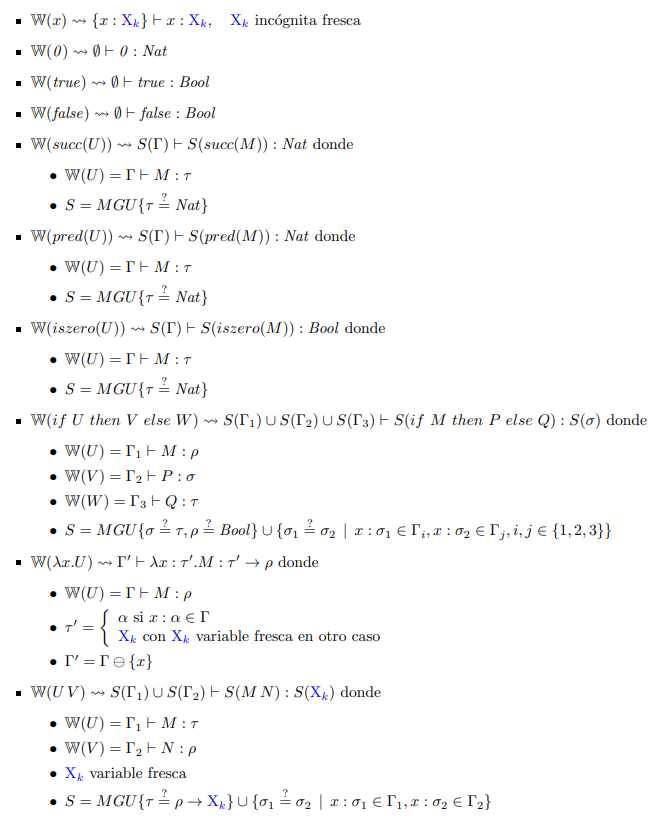
\includegraphics[width=\linewidth]{assets/algoritmo_w.png}
\end{minipage}

\textbf{Realmente Importante}: Recordemos que en los condicionales o cosas donde hay varios casos, cada tipo debe ser diferente aunque parezca obvio. Las restricciones se colocan luego. Nótese que en la segunda imagen, $U_{2}$ y $U_{3}$ son de tipos distintos $W(U_{2}) = \Gamma_{2} \vdash M_{2}:\tau_{2}$ y $W(U_{3}) = \Gamma_{3} \vdash M_{3}:\tau_{3}$ pero la restricción de como son se le da a la hora de hacer la sustitución $\{t_{2} = t_{3}\}$ \\
\textbf{Realmente Importante}: Como en los casos condicionales puede ser que una variable aparezca en más de una rama, tenemos que verificar que esa variable tenga el mismo tipo en todas las ramas. Esto se puede ver en la segunda imagen marcado en rojo. \\ Imaginemos que en U1, U2, y U3 tengamos apariciones de una misma variable pero con diferente tipo, esto no sería válido. \\
\textbf{Realmente Importante}: $\emptyset$ en el Algoritmo de W representa quitar una variable específica del contexto. Esto se ve fácil si de antemano vemos como es el juicio de tipado de la regla. 
\[\begin{minipage}[b]{0.7\textwidth}
    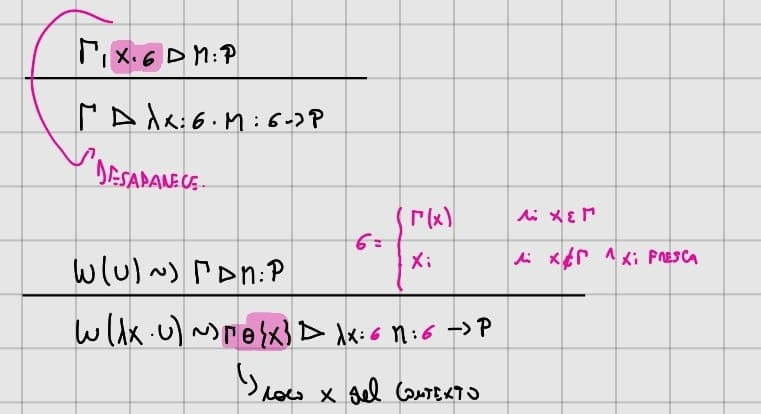
\includegraphics[width=\linewidth]{assets/abs_inf.jpg}
\end{minipage}\]

\subsubsection*{Incógnitas Frescas}
Las Incógnitas Frescas son variables de tipo que se introducen durante el proceso de inferencia para representar tipos que aún no se conocen. Que sea fresca garantiza que es única y no ha sido utilizada antes en el contexto de inferencia actual. 
\section*{Lógica de Primer Orden (LPO)}
Es prácticamente igual a la Lógica Proposicional pero acá se introducen los cuantificadores $\forall$ y $\exists$. En cuanto a tema de materia, es parecido a deduccion natural pero con cuantificadores. \\
Necesitamos entender la Lógica de Primer Orden porque es en lo que se basa Prolog (Programación Lógica) 
\subsection*{Lenguaje de Primer Orden $\mathcal{L}$}
Está formado por 
\begin{itemize}
    \item Conjunto de Símbolos de Función $\mathcal{F} = \{f, g, h, \dots\}$. Cada Símbolo de función tiene asociada una aridad ($\ge 0$)
    \begin{itemize}
        \item Los Símbolos de Función con aridad 0 se llaman \textbf{constantes}
    \end{itemize}
    \item Conjunto de Símbolos de Predicado $\mathcal{P} = \{P, Q, R, \dots\}$. Cada Símbolo de predicado tiene asociada una aridad ($\ge 0$)
    \item Conjunto Infinito de Numerable de Variables $ \mathcal{X} = \{X, Y, Z, \dots\}$
\end{itemize}
\textbf{Importante}: Los predicados solamente definen una relación entre dos elementos de mi dominio (devuelven un valor de verdad). La idea es enviar como argumento cosas que ya son irreducibles o pueden reducirse hasta poder compararse. \\
\textbf{Importante}: Las funciones solamente reciben como argumentos elementos de mi dominio y devuelven un elemento de mi dominio. Si se quisiese usar para una fórmula lógica ese valor, debería colocarse un predicado que nos arroje un valor de verdad para ese valor del dominio. 
\subsubsection*{Términos de Primer Orden}
Definimos el conjunto $\mathcal{T}$ de términos mediante la siguiente gramática $t :: = X \ | \ f(t_{1}, \dots, t_{n})$ donde \textbf{X} denota una variable y \textbf{f} un símbolo de función de aridad n. \\
\textbf{Importante}: Si un símbolo de función, llamémosle g tiene aridad 3, se debe usar enviando los 3 parámetros. Acá no existe la opción de algo ser opcional. \\
Véase \hyperref[subsec:terminos_lpo]{\textbf{\underline{anexo}}} para poder ver con más profundidad la justificación de qué es o no un término.
\subsubsection*{Diferencia entre Símbolo de Función y Símbolo de Predicado}
Un Símbolo de Función me devuelve un elemento de mi Dominio o universo. Los predicados no. \\
Ej.: $n, \ succ(n)$ son símbolos de función mientras que $\ge$ es un símbolo de predicado. 
\subsubsection*{Notación Infija, Prefija en LPO}
Ej.: $+(0, succ(X)) \equiv 0 + succ(X)$. Nosotros usaremos la notación infija. 
\subsubsection*{Fórmulas de Primer Orden}
\[\begin{minipage}[b]{0.7\textwidth}
    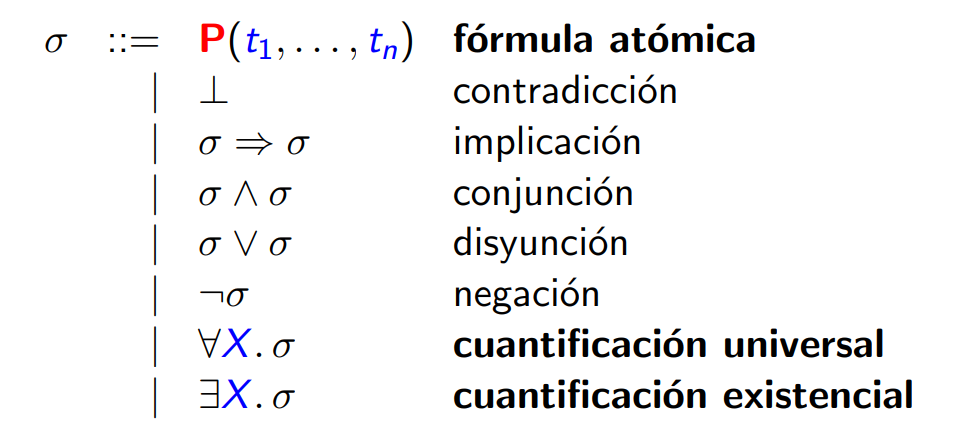
\includegraphics[width=\linewidth]{assets/formulas_lpo.png}
\end{minipage}\]
Al igual que en Cálculo Lambda, los cuantificadores ligan variables siempre y cuando esté definida en ese ámbito. En este caso, \textbf{X} está ligada; \textbf{P} denota un símbolo de predicado de aridad n. \\
\textbf{Importante}: Dos fórmulas que solo difieren en los nombres de las \textbf{variables ligadas} se consideran iguales. Esto es por el isomorfismo de las variables ligadas, da igual qué nombre tengan.
\subsubsection*{Sustitución}
Hay que tener cuidado en sustituir en LPO, si vamos a sustituir una variable que depende de otra que está ligada a un cuantificador, antes hay que renombrar la variable ligada en cuantificador. \\
Ej.: $\sigma := succ(X) = Y \implies \exists Z.X+Z = Y$\\
¿Qué es lo que sucede si hacemos $\sigma \{X:=Z*Z\}$? Cuando querramos reemplazar en el cuantificador del existe, el existe \textbf{ya tiene una Z} pero esta Z que está en el cuantificador es diferente a la que está en nuestro $\{X:=Z*Z\}$ por lo tanto hay que renombrar la Z del cuantificador porque de lo contrario, parecerá que son la misma. \\
El resultado de hacer esta operación quedaría como $\sigma := succ(Z*Z) = Y \implies \exists Z'.(Z*Z)+Z' = Y$ \\
\textbf{Importante}: Recordar que solamente reemplazamos las ocurrencias libres de una variable, no la que está ligada a un cuantificador. 
\subsection*{Deducción Natural extendida a LPO}
Todas las reglas de deducción natural proposicional siguen vigentes pero acá se agregan las reglas de introducción y eliminación para el $\forall$ y $\exists$. \\
Igual que antes: 
\begin{itemize}
    \item Un contexto $\Gamma$ es un conjunto finito de fórmulas.
    \item Un secuente es de la forma $\Gamma \vdash \sigma$
\end{itemize}
\[\begin{minipage}[b]{0.8\textwidth}
    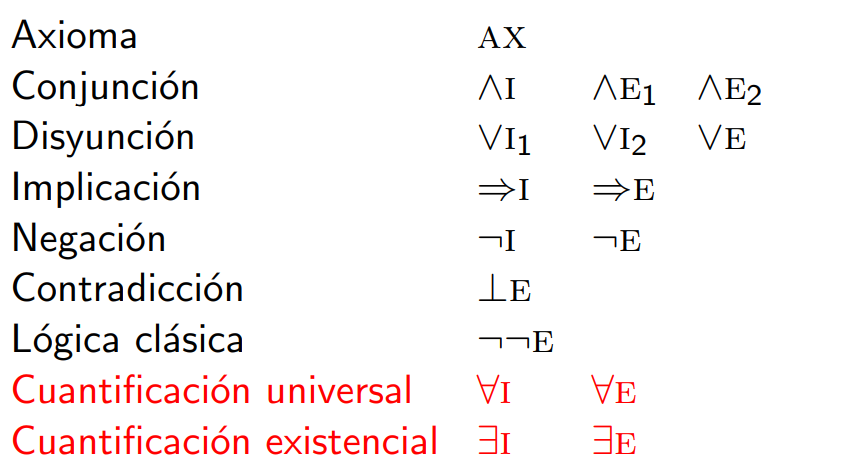
\includegraphics[width=\linewidth]{assets/reglas_deduccion_lpo.png}
\end{minipage}\]
\[\begin{minipage}[b]{0.8\textwidth}
    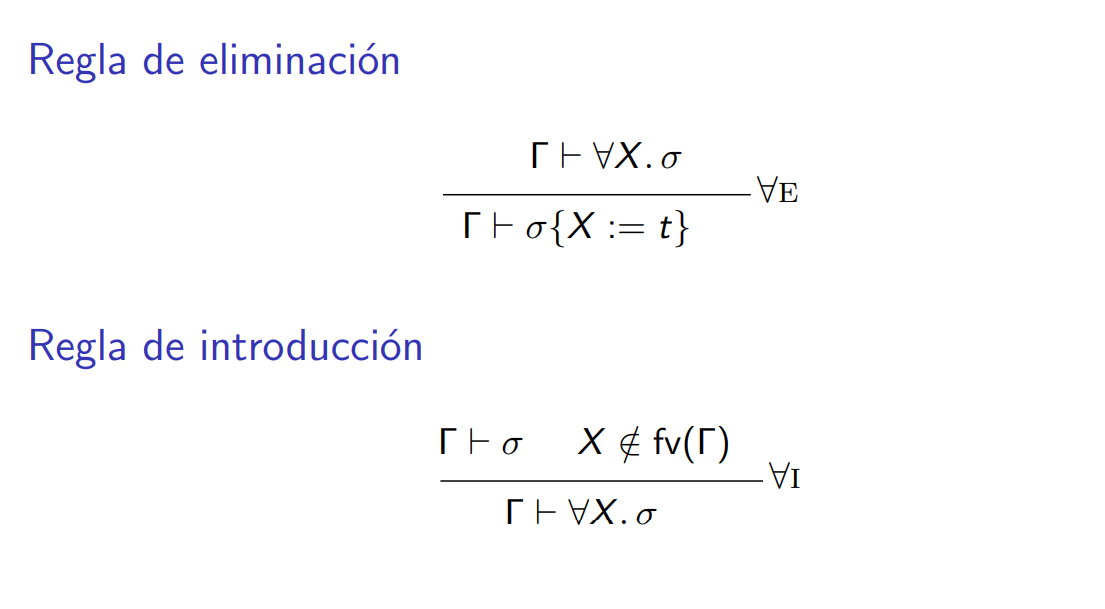
\includegraphics[width=\linewidth]{assets/reglas_deduccion_lpo_forall.png}
\end{minipage}\]
\[\begin{minipage}[b]{0.8\textwidth}
    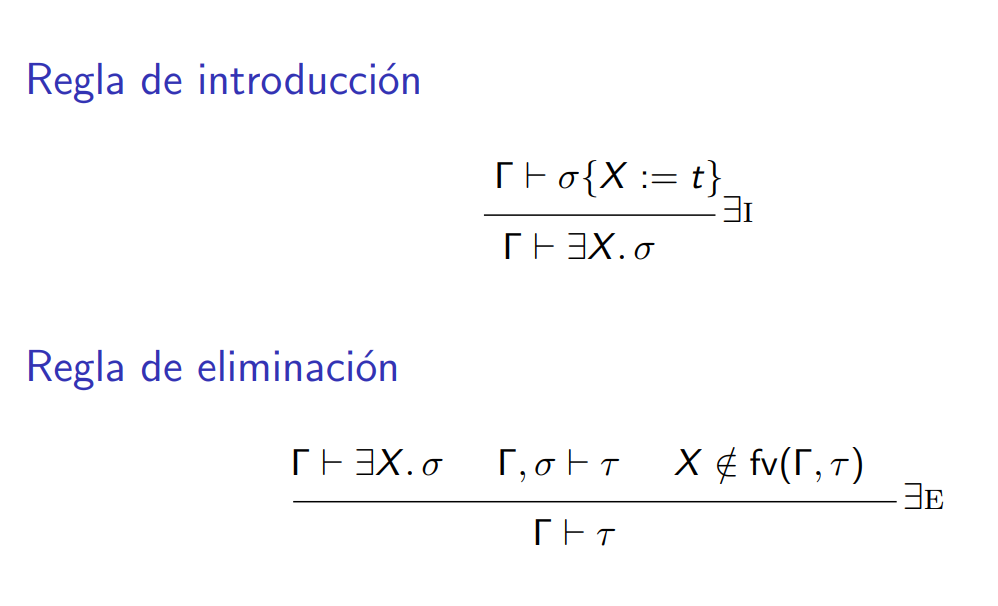
\includegraphics[width=\linewidth]{assets/reglas_deduccion_lpo_exists.png}
\end{minipage}\]
\subsection*{Estructuras de Primer Orden}
Nos ayuda a decir \textbf{cómo interpretamos} los elementos del universo (M, I). Definimos como \textbf{estructura de primer orden} como el par $\mathcal{M} = (M, I)$
\begin{itemize}
    \item $\mathcal{M}$: Conjunto \textbf{no vacío}, llamado universo.
    \item $\mathcal{I}$: Es una función que le da una interpretación a cada símbolo. 
    \item Para cada símbolo de función \textbf{f} de aridad n: $I(f): M^{n} \rightarrow M$
    \item Para cada símbolo de predicado \textbf{P} de aridad n: $I(P) \subseteq M^{n}$
\end{itemize}
¿Por qué es necesario esto? Hasta este momento $\forall X . X$ no nos dice nada. Es solo sintáxis. \\
Cuando hablamos de 0 podría significar falso en el ámbito o universo de los booleanos, podría significar 0 en los naturales. \\
Para poder darle todo este significado a cada símbolo tenemos que usar la función de interpretación. La función de interpretación es re importante, porque algo que está escrito de la misma manera puede ser verdadero o falso según en donde habitemos. 
\[\begin{minipage}[b]{0.8\textwidth}
    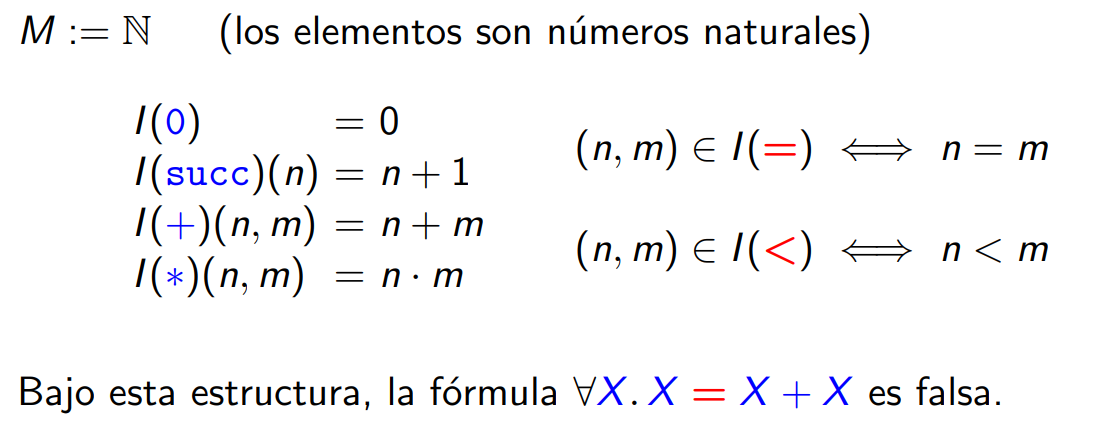
\includegraphics[width=\linewidth]{assets/universo_interprete.png}
\end{minipage}\]
\subsubsection*{Asignación}
Una asignación es una función que a cada variable le asigna un elemento del universo: $a: \mathcal{X} \rightarrow M$
\subsubsection*{Interpretación de Términos}
Cada término $t \in \mathcal{T}$ se interpreta como un elemento, extendiendo la definición de \textbf{a} a términos: $a(t) \in M$: $a(f(t_{1}, \dots, t_{n})) = I(f)(a(t_{1}), \dots, a(t_{n}))$
\subsubsection*{Interpretación de Fórmulas}
Suponemos fijada una estructura de primer orden $\mathcal{M} = (M, I)$. \\
Definimos una relación de \textbf{satisfacción a} $\vDash_{\mathcal{M}}\sigma$ $"$La asignación \textbf{a} (bajo la estructura $\mathcal{M}$ satisface la fórmula $\sigma$)$"$
\[\begin{minipage}[b]{0.8\textwidth}
    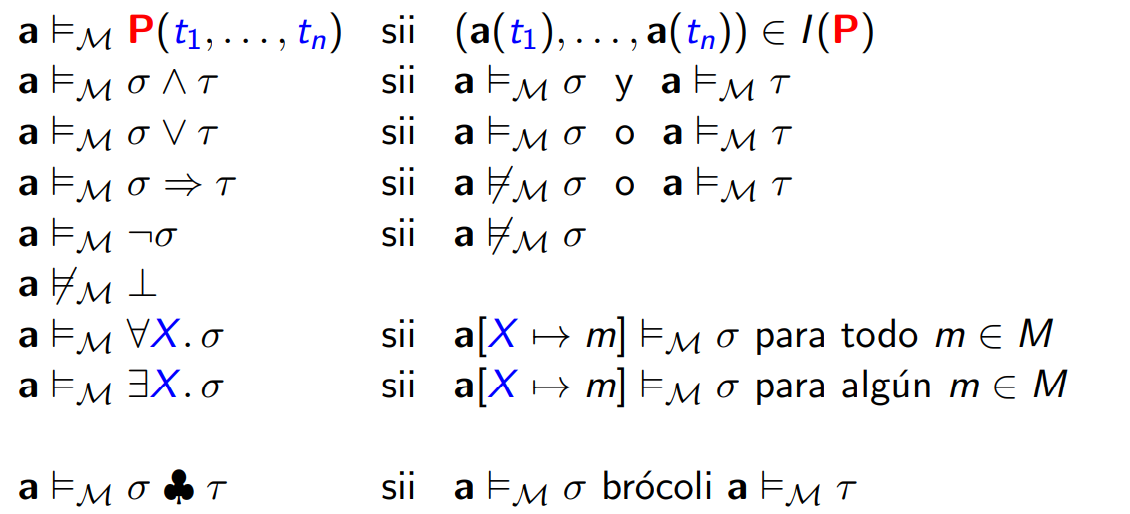
\includegraphics[width=\linewidth]{assets/interpretacion_formulas_lpo_deduccion_natural.png}
\end{minipage}\]
\textbf{Importante}: $a[x \rightarrow m]$ representa el mapsTo y está definido de la siguiente forma: \\
$a: V \rightarrow M$ \\
$a[x \rightarrow m]: V \rightarrow M$ \\
$a[x \rightarrow m](y) =
\begin{cases}
    m \ si \ x = y \\
    a \ si \ x \neq y
\end{cases}
$ \\
Véase \hyperref[subsec:lpo_formulas]{\textbf{\underline{anexo}}} para ver ejemplos de fórmulas válidas, aplicaciones de predicados y símbolos de función
\subsubsection*{Validez y Satisfactibilidad}
\[\begin{minipage}[b]{0.8\textwidth}
    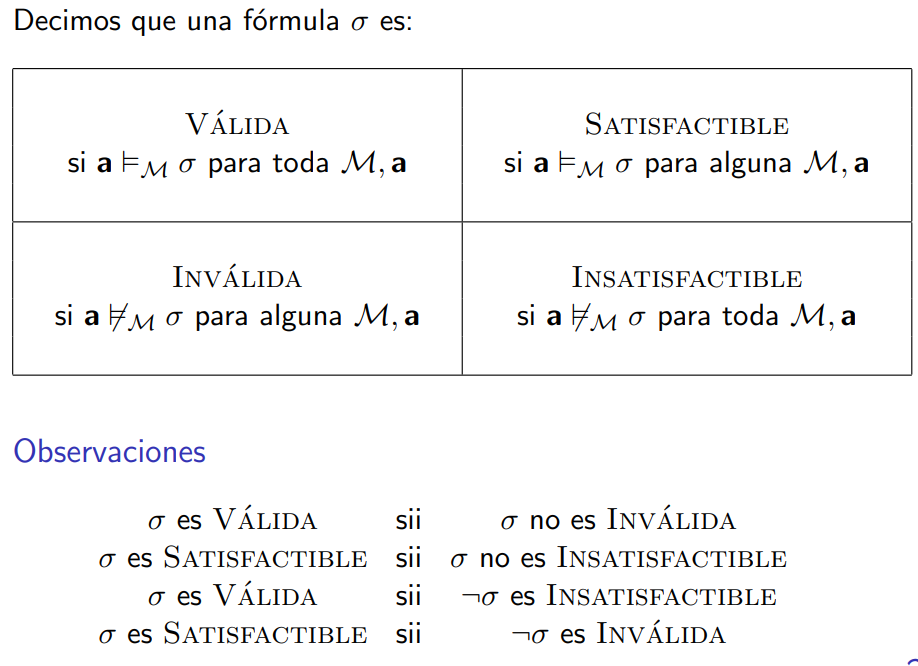
\includegraphics[width=\linewidth]{assets/validez_satisfactibilidad.png}
\end{minipage}\]
\section*{Pre-Prolog}
\subsection*{Términos de Primer Orden}
Prolog opera con ellos. Son de la pinta $X \ Y \ succ(succ(zero)) \ bin(I, R, D) \dots$
\subsection*{Fórmulas Atómicas}
En Prolog son de la forma $pred(t_{1}, ..., t_{n})$ \\
Ej.: $padre(zeus, atenea)$
\subsection*{Programa en Prolog}
Es un conjunto de reglas: $\sigma :- \tau_{1}, \dots, \tau_{n}$. \\
Cada $\sigma$ es una regla. \\
Ej.: $abuelo(X,Y) :- padre(X,Z), \ padre(Z,Y)$. En este caso $\sigma := abuelo(X,Y)$, $\tau_{1} := padre(X,Z)$ y $\tau_{2} := padre(Z, Y)$.  
\subsubsection*{Hechos}
Son aquellas reglas en las cuales $n = 0$. Es lo que se considera verdadero o tautológico. \\
¿A qué nos referimos con $n=0$? Bueno, que no dependen de nada. \\
Ej.: $\sigma :- padre(zeus, ares)$ 
\subsubsection*{Interpretación Lógica de las Reglas}
Cada uno de los $\tau$ en conjunción deben implicar $\sigma$ \\
Es decir, tienen la siguiente interpretación lógica $\forall X_{1}, \dots \forall X_{k}((\tau \land \dots \land \tau_{n}) \implies \sigma)$ donde $X_{1}, \dots, X_{k}$ son todas las variables libres de las fórmulas. \\
Ej.: $\forall X . \forall Y . \forall Z . ((padre(X,Z) \land padre(Z,Y)) \implies abuelo(X,Y))$
\subsubsection*{Consultas}
Hablamos de Consultas en Prolog cuando aparece una incógnita X. \\
Una consulta es de la forma: $?- \sigma_{1}, \dots, \sigma_{n}$ \\
Ej.: $?-abuelo(X, ares)$ 
\subsubsection*{Interpretación Lógica de las Consultas}
El X hay que predicarlo en base a existenciales. \\
Ej.: $\exists X_{1}, \dots, \exists X_{k} . (\sigma_{1} \land \dots \land \sigma_{n})$ donde $X_{1}, \dots, X_{k}$ son todas las variables libres de las fórmulas. \\
\subsubsection*{Claúsula y Literales}
\textbf{Claúsula}: $(P \land Q)$. \\
\textbf{Literal}: $P$
\subsection*{Lógica Proposicional}
\subsubsection*{Pasaje de Logica Proposicional a Forma Clausal}
Es un algoritmo. \\
La entrada es una \textbf{fórmula $\sigma$ de la lógica proposicional} y la salida es un booleano que indica si $\sigma$ es válida. 
\begin{itemize}
    \item Reescribir los $\implies$: $a \implies b \equiv \neg a \lor b$
    \item Pasar a Forma Normal (f.n) Negada: Empujar los $\neq$ hacia adentro (si hay).
    \item Pasar a Forma Normal (f.n) Conjuntiva: Distrubuir $\lor$ sobre $\land$ (si hay).
\end{itemize}
Luego, la forma Clausal está formada por conjunciones de disyunciones. \\
Ej.: $(p \lor q) \land (q \lor r)$ en Forma Clausal es $\mathcal{C} = \{\{p,q\}, \{q, r\}\}$. En este caso, esta Forma Clausal está dado por 2 Cláusulas, donde cada Claúsula tiene 2 literales.
\subsubsection*{Prioridad de Formas Normales en Logica Proposicional}
Hay tantas que puede ser un quilombo pero es así: $negada  \subseteq conjuntiva$
\subsubsection*{Refutación (Método de Resolución) en Lógica Proposicional}
Llamemos $\sigma$ a una fórmula de la lógica proposicional cualquiera. \\
\textbf{Refutación de $\mathcal{C}$}: Derivación de $\mathcal{C} \vdash \bot$ \\
Si encontramos una refutación de $\mathcal{C}$: 
\begin{itemize}
    \item Vale $\neg \sigma \vdash \bot$: Es decir, $\neg \sigma$ es insatisfactible o contradicción.
    \item Luego, vale $\vdash \sigma$. Es decir, $\sigma$ es tautología.
\end{itemize}
Si NO encontramos una refutación de $\mathcal{C}$:
\begin{itemize}
    \item No vale $\neg \sigma \vdash \bot$. Es decir, $\sigma$ es satisfactible.
    \item Luego, no vale $\vdash \sigma$. Es decir, $\sigma$ no es válida.
\end{itemize}
Es un algoritmo y tiene varios pasos pero veamos un ejemplo. \\
Ej.: $(P \land Q) \implies P$ ¿Cuáles son tautologías?  Si nos está pidiendo cuales son tautologías tenemos que ver que $\neg \sigma$ sea insatisfactible o contradicción, si esto sucede entonces $\sigma$ es tautología. \\
Lo primero que hacemos es pasar la fórmula $\neg \sigma$ a Forma Clausal, por el algoritmo descripto anteriormente nos queda
\begin{itemize}
    \item $\neg ((P \land Q) \implies P)$
    \item Eliminación del $\implies$: $\neg (\neg(P \land Q) \lor P)$
    \item Empujar $\neg$ interno: $\neg (\neg P \lor \neg Q \lor P)$
    \item Empujar $\neg$ externo: $P \land Q \land \neg P$
\end{itemize}
Luego, la forma Clausal es $\mathcal{C} = \{\{P\}, \{Q\}, \{\neg P\}\}$ \\
Ahora básicamente tenemos que ir eligiendo cláusulas \textbf{k} y \textbf{k'} hasta que lleguemos al vacío. \\
Eligiendo $k=\{P\}$ y $k'=\{\neg P\}$ nos da $\emptyset$. Por lo tanto, se agrega $\emptyset$ a $\mathcal{C}$ pero en el paso recursivo, como $\emptyset$ pertenece a $\mathcal{C}$ llegamos a que $\neg \sigma$ es insatisfactible. Luego, $\sigma$ es tautología. \\
\textbf{Importante}: Es útil ver que para llegar a vacío no siempre es necesario usar todas las cláusulas. Inclusive, va a haber veces que jamás se llegue a insatisfactible. Entonces eso indicaría que si vale $\neg \sigma$ entonces $\sigma$ es inválida. \\
\textbf{Importante}: Este proceso siempre termina.
\subsection*{Lógica de Primer Orden (LPO)}
\subsubsection*{Pasaje de LPO a Forma Clausal}
Es prácticamente un algoritmo. Es parecido al anterior en los primeros 2 pasos. La diferencia es que acá si $\sigma$ no es válida, el método puede no terminar. \\
En la teórica les ponen los pasos de una, pero a mí no me gustó como lo ordenaron. Primero lean lo de abajo, y va a haber una sección que se llama igual que esta pero con un (2). 
\subsection*{Resolución para Lógica de Primer Orden}
Hay que pasar por varias formas hasta llegar a la forma Clausal.
\textbf{Importante}: Lo anoto en todos lados porque siempre me olvido. No por algo nos hacen detectar siempre las variables ligadas y libres. Si tenés más de un cuantificador con la misma variable, entonces renombrá algun cuantificador y reemplazá su ocurrencia por la nueva variable, porque después es un quilombo.
\subsubsection*{Pasaje a forma clausal en Lógica de Primer Orden}
\subsubsection*{Skolemización}
La Skolemización es deshacerse de los cuantificadores existenciales. \\
La idea es introducir testigos para los $\exists$ sin cambiar la satisfactibilidad. 
\begin{itemize}
    \item Todo cuantificador existencial se instancia en una constante o función de skolem.
    \begin{itemize}
        \item Utilizamos una función cuando el cuantificador existencial está dentro al alcance de un cuantificador para todo (el más cercano). 
        \item Utilizamos simplemente c cuando el cuantificador existencial no está al alcance de otro cuantificador.
    \end{itemize}
\end{itemize}
\textbf{Importante}: La Skolemización \textbf{no es determinística}. \\
\textbf{Importante 2}: Skolemizar de afuera hacia adentro. \\
\textbf{Importante 3}: La Skolemización \textbf{preserva la satisfactibilidad} pero \textbf{no produce fórmulas equivalentes}, esto quiere decir que no preserva la validez. Ej.: $\exists X . (P(0) \implies P(X))$ es válida mientras que $P(0) \implies P(c)$ es inválida. \\
Ejemplo de Skolemización con existenciales sin alcance de universales
\[\begin{minipage}[b]{0.2\textwidth}
    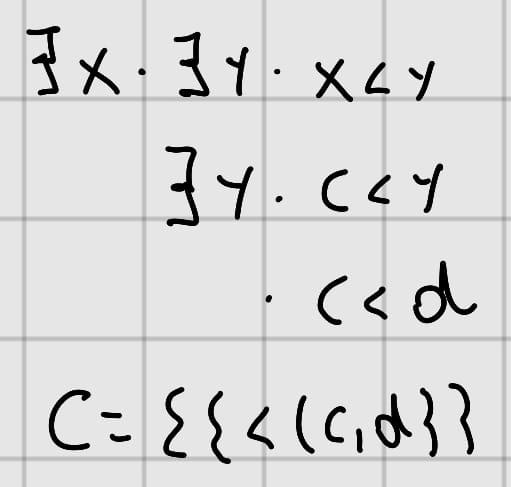
\includegraphics[width=\linewidth]{assets/skolem_1.jpg}
\end{minipage}\]
Ejemplo de Skolemización con existenciales al alcance de universales
\[\begin{minipage}[b]{0.6\textwidth}
    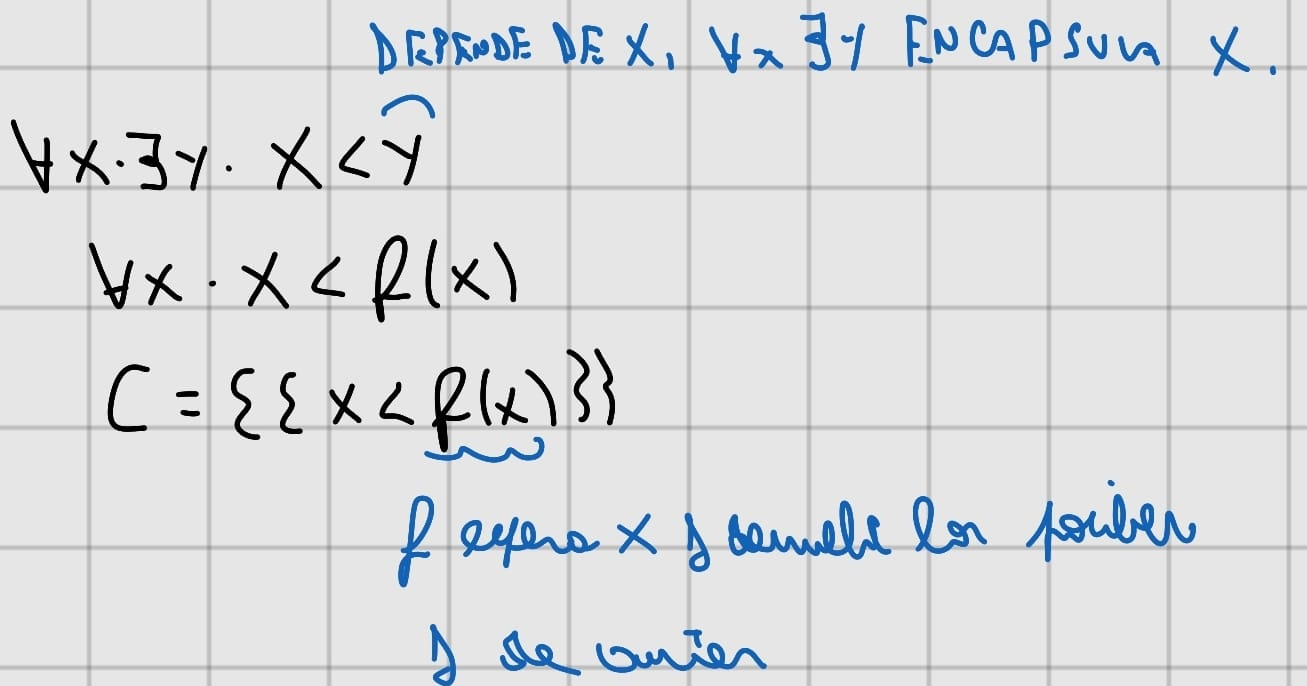
\includegraphics[width=\linewidth]{assets/skolem_2.jpg}
\end{minipage}\]
\subsubsection*{Forma Normal de Skolem (NNF)}
Sea A una sentencia rectificada en FNN. Una fórmula está rectificada si todos sus cuantificadores ligan variables distintas entre sí, y a la vez distintas de todas las variables libres. \\
\textbf{En criollo}: Los cuantificadores tienen variables con nombres únicos y no se pisan con variables libres. \\
Una fórmula en forma normal de Skolem tiene la siguiente pinta: $\sigma_{Sk} :: = \forall X_{1}X_{2} \dots \ X_{n} * \tau$
\subsection*{Pasaje de LPO a Forma Clausal (2)}\begin{itemize}
    \item Reescribimos $\implies$ usando $\neg$ y $\lor$.
    \item Pasar a f.n negada, empujando $\neg$ hacia adentro.
    \item Pasar a f.n extrayendo $\forall$ y $\exists$ hacia afuera.
    \item Pasar a f.n de Skolem, Skolemizando los existenciales.
    \item Pasar a f.n. conjuntiva, distribuyendo $\lor$ sobre $\land$.
    \item Empujar los cuantificadores hacia adentro de las conjunciones.
\end{itemize}
Acá dejo una imagen que hice por si es de utilidad, con las propiedades y todo (res: es lo que te devuelve al aplicar ese paso)
\[\begin{minipage}[b]{1\textwidth}
    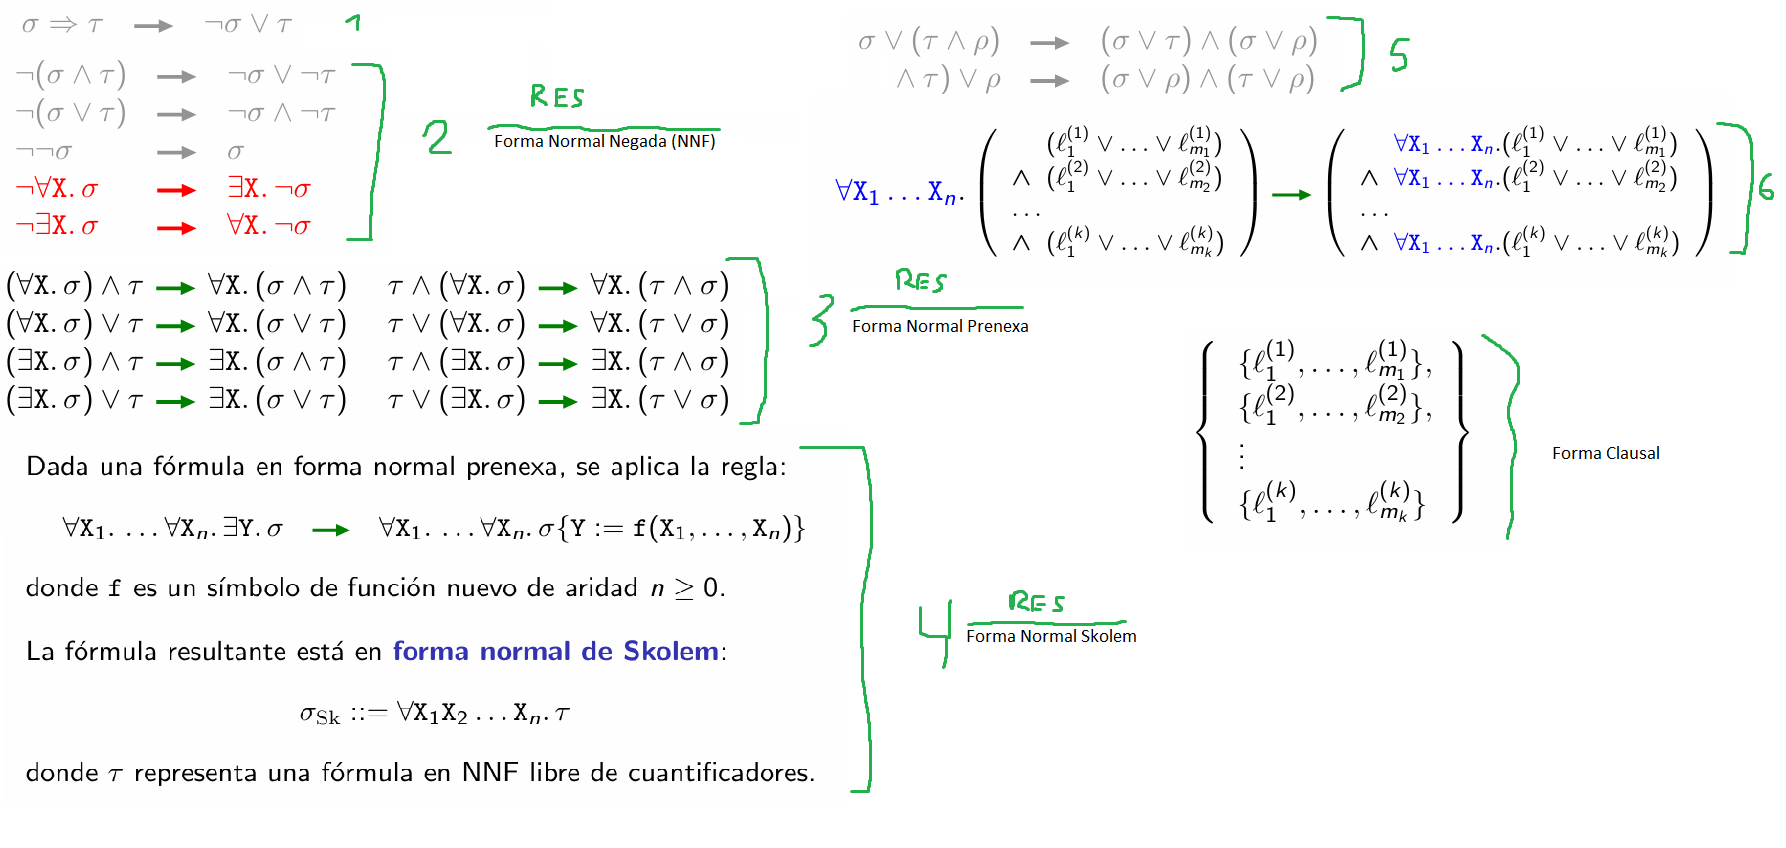
\includegraphics[width=\linewidth]{assets/paso_paso_lpo_clausal.png}
\end{minipage}\]
Véase \hyperref[subsec:lpo_forma_clausal]{\textbf{\underline{anexo}}} para dos ejemplos
\subsubsection*{Prioridad de Formas Normales en LPO}
Hay tantas que puede ser un quilombo pero es así: $negada \subseteq prenexa \subseteq skolem \subseteq conjuntiva$
\subsubsection*{Refutación (Método de Resolución) en LPO}
Es exactamente igual que en Lógica Proposicional \textbf{excepto} que ahora como existen funciones P que tienen argumentos, hay que ver si los argumentos son unificables. \\
Hasta ahora, esto vale $\forall X . P(X) \land \neg P(0)$, esto es porque las claúsulas que tenemos son $\mathcal{C} = \{\{P(X)\}, \{\neg P(0)\}\}$ y la regla propuesta no aplica porque las P son iguales pero sus argumentos no. \\
Ej.: Sea $\neg \sigma$ con sus cláusulas, $\mathcal{C} = \{\{P(X,Y)\}, \{\neg P(f(z), Z)\}\}$
\begin{itemize}
    \item Para cancelar los términos opuestos $P$ y $\neg P$, unificamos.
    \item $mgu(P(X,Y) \stackrel{?}{=}P(f(Z), Z))$. Para que estos sean iguales en argumento vemos que unificamos como $\{X := f(z), Y := Z\}$.
    \item Luego, k = $P(f(z), Z)$ y k' = $\neg P(f(z), Z)$ nos da como resultado $\{\}$ o $\emptyset$.
    \item Por lo tanto como $\neg \sigma$ es insatisfactible, $\sigma$ es tautología.
\end{itemize}
\textbf{Importante}: Primer paso de todo ejercicio: si comenzamos teniendo implicaciones, o cuantificadores universales existenciales con las mismas variables, recordar renombrarlas. \\
\textbf{Importante2}: (A nivel MGU) Si hay un cuantificador existencial que ahora depende un universal, primero hay que chequear \textbf{en qué términos} se usa la variable \textbf{ligada al cuantificador universal}. Esto es, porque cuando eliminemos el \textbf{cuantificador existencial}, la existencial se elimina y será del tipo \textbf{f(variableCuantUniversal)} pero como variableCuantUniversal estaba en otro término (no ligado al existencial) al intentar unificar nos dará occurs-check pues variableCuantUniversal NO unifica con f(variableCuantUniversal). La idea justamente acá, es que como el existencial asegura que existe (puede no existir), entonces no podemos confundir con la ligada al para todo porque esa sí vale siempre. Igual, dejo un ejemplo acá abajo.
\[\begin{minipage}[b]{1\textwidth}
    \includegraphics[width=\linewidth]{assets/lpo_skolem.jpg}
\end{minipage}\]
OJO. Esto es SOLO a nivel MGU. Con esto quiero decir que si vas a unificar, le cambies el nombre a las variables. 
\section*{Prolog}
El algoritmo que vimos antes para ver si una fórmula de primer orden $\sigma$ es válida funciona, pero es costosa. Esto es porque a nivel computacional implica hacer
\begin{itemize}
    \item Búsqueda: Elegir dos claúsulas
    \item Selección: Elegir un subconjunto de literales de cada claúsula
\end{itemize}
Además en cada paso se agrega una claúsula, resolverse ecauciones de unificación y se usa BFS.\\
¿Cómo soluciona este problema Prolog? Usando \textbf{resolución SLD}.
\subsection*{Resolución SLD}
La resolución SLD se aplica solamente sobre cláusulas de Horn. 
\subsection*{Cláusulas de Horn}
Recordemos que una claúsula es un conjunto de literales 
\[\{l_{1}, \dots, l_{n}\}\]
Los literales son de la forma 
\[l::= P(t_{1}, \dots, t_{n})\ |\ \neg P(t_{1}, \dots, t_{n})\]
En SLD cada cláusula tiene como máximo un literal positivo. \\
Por ejemplo, en SLD no es posible resolver esto: $\mathcal{C} = \{\{P(X), Q(Y)\}, \{\neg Q(Y)\}\}$ porque la primera claúsula tiene dos positivos. 
\subsubsection*{Grupos en Claúsulas de Horn}
\begin{itemize}
    \item Las que tienen un literal positivo y ningún negativo se llaman hechos o axiomas.
    \begin{itemize}
        \item En LPO: $\{P(X)\}$
        \item padre(m, t): Es un axioma que dice que m es padre de t.
        \item madre(k, t): Es un axioma que dice que k es madre de t.
    \end{itemize}
    \item Las que tienen un literal positivo y una/varias negativas se llaman reglas.
    \begin{itemize}
        \item En LPO: $\{P(X), \neg Q(X,Y)\}$
        \item En Prolog: padres(x) :- madre(m, x), padre(p, x).
        \item Esta regla define que x tiene 'padres' cuando existe una madre m de x y un padre p de x.
    \end{itemize}
    \item Las que NO tienen literal positivo y una/varias negativas se llaman cláusulas objetivo.
    \begin{itemize}
        \item En LPO: $\{\neg P(X)\}$
        \item padres(t).
        \item Cuando esto le llega a Prolog, se conforma una claúsula objetivo que se compone de literales negativos.
    \end{itemize}
\end{itemize}
\textbf{Nota}: Los axiomas + reglas en Prolog se llaman \textbf{cláusulas de definición (PGM)} y estas nunca llegan a ser insatisfactibles. 
\subsubsection*{Derivación SLD}
En cada paso, Prolog siempre toma una \textbf{claúsula de definición (PGM)} y una \textbf{claúsula objetivo (Goal)}
\section*{Programación Orientada a Objetos (POO)}
No subieron la teórica así que voy a tener que escribir en base a lo que anoté yo y me pareció interesante. \\
Vamos a usar SmallTalk donde todo es prácticamente un objeto. \\
En SmallTalk los objetos se comunican entre sí a través de mensajes, donde cada mensaje es una invocación a un método de un objeto. \\
Como en el Paradigma Orientado a Objetos podemos mutar instancias de objetos determinados a través de métodos (getters/setters), necesitamos tener un estado. Al principio de la materia vimos que el estado no es más que el conjunto o estado de variables en un momento dado. 
\subsection*{Mensajes}
Siempre están asociados a un objeto.
\subsection*{Métodos de Instancia y Métodos de Clase}
Los métodos no son más que la implementación de la respuesta a un mensaje dado. \\
\begin{lstlisting}
    Object subclass: Persona [
        Persona class >> hola [
            ^'hola, como estas'
        ]

        Persona class >> crearNuevaPersona [
            ^Persona new.
        ]
    ]

    obj := Persona new.
    obj hola.
\end{lstlisting}
En este caso el mensaje es hola (invocar al método de instancia hola), y la respuesta 'hola, como estas' la devuelve el método hola de la clase persona. \\
La diferencia entre un método de instancia y método de clase es la siguiente 
\begin{itemize}
    \item Método de Instancia: Son métodos que se pueden ejecutar \textbf{a través de la instancia de una clase}.
    \begin{itemize}
        \item Ej.: obj hola.
    \end{itemize}
    \item Método de Clase: Se ejecutan en la clase misma, y nos pueden ayudar a la creación de nuevas instancias.
    \begin{itemize}
        \item Ej.: obj := Persona crearNuevaPersona.
    \end{itemize}
\end{itemize}
\subsection*{Objeto Receptor}
Es el objeto que recibe el mensaje. Puede recibirlo tanto una clase a través de un método de clase, o una instancia de la clase a través de un método de instancia. 
\subsection*{Objeto Colaborador}
Es un objeto con el que el receptor interactúa o colabora para lograr una tarea o propósito. \\
Es un parámetro. Ej.: 10 mcm: 4, 4 actúa como colaborador.
\subsection*{Return}
En el código, el return se puede notar como $\land \ variable$
\subsection*{Uso de Variables en Clases}
No nos referimos a ella como this, como si hacemos en muchos lenguajes, sino que acá, en SmallTalk simplemente mencionamos la variable. 
\subsection*{POO y Clean Code}
Jamás, bajo ningún termino agregamos campos a una clase por fácilidad de cómputo. Las variables que representan a una clase deben ser la menor cantidad, y deben estar pensadas para el objetivo que tenga ese objeto de resolver. \\
Esto es más que nada porque, un objeto debería ser lo más chico posible además de que si agregamos campos extra, hay que mantenerlos y eso da un costo mayor. 
\subsection*{Tipos de Expresiones en SmallTalk}
\begin{itemize}
    \item Variables Locales: Se escriben en minúscula 
    \begin{itemize}
        \item x:=3. y:=2.
    \end{itemize}
    \item Variables Globales: Se escriben en mayúscula (no obligatorio). Se definen a nivel de clase, y son accesibles desde cualquier parte del programa a través de la clase a la que pertenecen.
    \begin{itemize}
        \item classVariableNames: 'contador'
    \end{itemize}
    \item Mensajes Unarios: Toman un único parámetro. Se usan de manera prefija.
    \begin{itemize}
        \item 10 print. Imprime el valor 10.
        \item 5 isOdd. Devuelve true. 
        \item -1. Devuelve el número -1, el (-) es un mensaje unario.
    \end{itemize}
    \item Mensajes Binarios: Toman dos parámetros. Se usan de manera infija.
    \begin{itemize}
        \item 3 + 5.
        \item 10 * 2.
        \item true and: false. 
    \end{itemize}
    \item Mensajes Keyword: Pueden tener múltiples argumentos, con cada argumento despues de su palabra clave correspondiente. 
    \begin{itemize}
        \item Rectangulo new ancho: 5 alto:10. Los keywords son ancho y alto.
    \end{itemize}
    \item Asignación
    \begin{itemize}
        \item persona := Persona new
    \end{itemize}
\end{itemize}
La prioridad, dentro de una expresión es la siguiente: $unarios > binarios > keyword$ \\
Veamos un ejemplo donde tiene importancia esto: Sea una clase de un entero, implemente un método de instancia que permita saber cual es el mcm del número instanciado y otro que viene por parámetro. \\
\begin{lstlisting}
    mcm: numberTwo 
        | res | 
        res := self * b // self gcd: b
        ^res
\end{lstlisting}
Como está implementado este código va a fallar, porque primero va a hacer self * b, e inmediatamente va a querer dividir por algo que todavía no se resolvió. 
\begin{lstlisting}
    mcm: numberTwo 
        | res |
        res := self * b // (self gcd: b)
        ^res
\end{lstlisting}
\textbf{Importante}: Nótese que todos los métodos los estamos haciendo dentro de una clase. Esto quiere decir que siempre tenemos que asumir que estamos dentro de un objeto. \\
Si tuviesemos que notar qué mensajes, receptores, colaboradores, resultados hay para la siguiente entrada: $6 \ mcm \ 10 $
\begin{itemize}
    \item Mensaje: mcm | Receptor: 6 | Colaboradores: 10 | Resultado: 30
    \item Mensaje: * | Receptor: Self (6) | Colaboradores: 10 | Resultado: 60 
    \item Mensaje: gcd | Receptor: Self (6) | Colaboradores: 10 | Resultado: 2
    \item Mensaje: // | Receptor: 60 | Colaboradores: 2 | Resultado: 30 
\end{itemize}
Nótese que básicamente fuimos paso a paso viendo qué instrucciones estaban y quienes estaban involucrados. 
\subsection*{Palabras Reservadas en SmallTalk}
\begin{itemize}
    \item true
    \item false
    \item self
    \item super
    \item nil
    \item thisContext
\end{itemize}
\subsection*{Algunos ejemplos de instancias de objetos}
\begin{itemize}
    \item nil: Es la instancia de UndefinedObject
    \item true: Es la instancia de la clase True 
    \item false: Es la instancia de la clase False
    \item Constantes Númericas: 1, 12, 125... son números, instancias de clases como SmallInteger o LargeInteger.
    \item Strings: $'hola'$ es la instancia de la clase String
    \item Símbolos: \#Rectángulo. Instancia de la clase Symbol. Un Símbolo es un objeto que representa un identificador único e inmutable. 
    \item Caracteres: \$a es la instancia de la clase Character. Representa un único caracter.
\end{itemize}
\subsection*{Herencia}
Importante: En la materia no se lo menciona, pero siempre es mejor priorizar la composición antes que la herencia. \\
La Herencia trae muchos problemas a nivel de objetos porque se vuelve inmantenible si la clase padre tiene muchos atributos, y esto es importante, porque una clase no debería estar abierta a eliminar cosas núcleo pero sí abierta a extenderla. \\
Esto es porque si refactorizamos la clase padre, si hay mas de una clase que heredaban esta, vamos a tener que considerar modificar andá a saber cuantas más clases. \\
El concepto de Herencia es importante, porque cuando hablamos de una relación padre-hijo, si desde hijo queremos llenar campos que están en el padre, usamos la palabra super, mientras que si queremos hablar de nuestro ámbito local de objeto usamos self. \\
Voy a mostrar un ejemplo en un lenguaje que conozca bien (TypeScript) para que después puedan relacionarlo en cualquier lenguaje. 
\begin{lstlisting}
    class ContactoBasico {
        msg: string;

        constructor(data){
            this.msg = data.msg;
        }
    }

    class ContactoEmail extends ContactoBasico {
        email: string;

        constructor(data){
            super(data);
            this.email = data.email;
        }

        hacerAlgo(){
            console.log(`Email: ${this.email}, Mensaje: ${this.msg}`);
        }
    }
\end{lstlisting}
En el ejemplo anterior, podemos ver que ContactoEmail puede almacenar un valor en msg como si fuese una variable de clase de sí misma, pero en realidad, esta puede ser utilizada a nivel ContactoEmail porque la estamos llenando vía super.
\subsection*{Self}
Cuando hablamos de Self, estamos hablando de utilizar las variables o métodos de la instancia del objeto que estamos manipulando. \\
El Self siempre busca hacia abajo. 
\subsection*{Super}
Cuando hablamos de Super, estamos hablando de herencia. Esto quiere decir que si una clase habla de super, está extendiendo de otra. Ojo, super habla de la clase inmediatamente que está por encima. \\
Esto es súper importante, porque hay muchos lenguajes (y gracias a dios) que no aceptan herencia múltiple. 
\begin{lstlisting}
    class ContactoBasico {
        msg: string;

        constructor(data){
            this.msg = data.msg;
        }

        hacerAlgo(){
            console.log("Hola");
        }
    }

    class ContactoEmail extends ContactoBasico {
        email: string;

        constructor(data){
            super(data);
            this.email = data.email;
        }

        hacerAlgo(){
            console.log(`Email: ${this.email}, Mensaje: ${this.msg}`);
        }
    }

    class ContactoEmailMasComplicado extends ContactoEmail {
        emailSecundario: string; 

        constructor(data){
            super(data);
            this.emailSecundario = data.emailSecundario;
        }

        hacerAlgo(){
            return super.hacerAlgo();
        }

    }
\end{lstlisting}
Ojo. En este ejemplo, si queremos instanciar ContactoEmailMasComplicado tendremos que cumplir la precondición de super, es decir, el constructor de ContactoEmail, y a su vez el de ContactoBásico. Esto es porque es una cadena. Ya se dan cuenta del por qué es malo laburar con herencia. \\
¿Qué es lo que sucede, si una vez instanciada ContactoEmailMasComplicado en obj, llamamos obj.hacerAlgo? ¿Qué hacerAlgo ejecuta?, bueno, el padre inmediato. Ejecutaría  console.log(`Email: ${this.email}, Mensaje: ${this.msg}`), es decir, el hacerAlgo() que está en ContactoEmail, que es padre de ContactoEmailMasComplicado. 
\subsection*{Importancia del Return}
En los métodos de una clase, si no tenemos un return, entonces el método retornará \textbf{self}. Es decir, la instancia. 
\subsection*{Métodos de Clase}
Los métodos de clase nos permiten crear instancias de una clase sin utilizar desde fuera de la clase la palabra reservada \textbf{new}. Esto nos permite que la clase por sí misma, diga qué es lo que podemos usar para crear instancias de ella. 
\begin{lstlisting}
    Object subclass: #Rectangulo 
            instanceVariableNames: 'ancho alto'
            classVariableNames: ''

    Rectangulo class >> ancho: ancho alto: alto [
        ^self new 
            ancho: ancho;
            alto: alto;
            yourself.
    ]

    Rectangulo >> ancho: valor [
        ancho := valor
    ]

    Rectangulo >> alto: valor [
        alto := valor
    ]

    Rectangulo >> descripcion [
        ^'Rectángulo de ancho ', ancho printString, ' y alto ', alto printString
    ]

    Uso: 
    rect := Rectangulo ancho: 30 alto: 20.
    rect descripcion.


\end{lstlisting}
Importante notar, que cuando hacemos $\land self \ new \ ancho: ancho;$ estamos creando una nueva instancia, mandando un mensaje al método ancho con el parámetro ancho. \\
Importante notar también, que cuando hacemos self new, estamos enviando un mensaje de new con varios argumentos. Estos argumentos los separamos por ; porque son parte del mismo mensaje.
\subsection*{Sobrecarga}
Decimos que un método de clase está sobrecargado cuando existe más de un método con el mismo nombre pero que toman diferentes parámetros (ya sea en cantidad o en tipos, lo importante es que no sean la misma cantidad de parámetros en el mismo orden y mismo tipo). Es importante notar que los métodos de clase más restrictivos deberían poder estar encapsulados en el más general. 
\begin{lstlisting}
    object subclass #robot 
           instance variablenames: 'posicion'

           inicializar: unaposicion
              posicion := unaposicion 

           posicion:
              ^posicion 
    
            inicializar:
                self inicializar: (0 @ 0)
\end{lstlisting}
\subsection*{Sintaxis de SmallTalk}
\begin{itemize}
    \item Usá \textbf{.} para indicar donde termina una instrucción. Es similar al \textbf{;} de C++ pero acá, si hay solamente una línea el \textbf{.} no es necesario.
    \begin{itemize}
        \item Ej.: 	x := 10. y := 20.
    \end{itemize}
    \item Usá \textbf{;} cuando tengas que encadenar mensajes a un mismo objeto, sin finalizar la ejecución de la expresión anterior. 
    \begin{itemize}
        \item Ej.: Transcript show: 'Hola'; cr; show: 'Mundo'
    \end{itemize}
\end{itemize}
\subsection*{Bloques (Block-Closures)}
Permite encapsular lógica dentro de un código independiente y reutilizable. Está compuesto por una secuencia de instrucciones que se agrupan y pueden ser pasadas como argumentos a métodos o invocadas como acción dentro de un método. \\
La sintáxis está compuesta por :variable + expresión \\
Si solo hay que definirlo, lo terminamos con \textbf{.}
\begin{lstlisting}
    [:x | x * 2]
\end{lstlisting}
Si hay que pasarle argumentos, lo invocamos con \textbf{:}
\begin{lstlisting}
    resultado := (1 to: 3) collect: [:x | x * 2].
    resultado tiene [2, 4, 6]
\end{lstlisting}
Si hay que obtener el resultado de un bloque, colocamos value antes del \textbf{.}. \\
El value invoca al bloque. Un value vacío es llamar al método sin argumentos.
\begin{lstlisting}
    resultado := [1 + 2 + 3] value. 
    resultado tiene el valor de 6
\end{lstlisting}
Si hay que usarlo en condicionales, cada rama podría ser un bloque 
\begin{lstlisting}
    resultado := 10 > 5 
        ifTrue: ['es mayor']
        ifFalse: ['es menor'].
\end{lstlisting}
Si hay que enviarle argumentos a los bloques, los enviamos a través de value, es decir, invocamos al bloque con tantos argumentos instanciados.
\begin{lstlisting}
    resultado := [:x :y | x+y ] value: 3 value: 4.
\end{lstlisting} 
Si querés usar variables locales en los bloques, la sintaxis es diferente 
\begin{lstlisting}
    resultado := [ | x y | x:= 3. y:=2. x+y. ]
\end{lstlisting}
\textbf{Importante}: Si un bloque está definido para n argumentos, solo se podrá invocar ese bloque enviando los n argumentos.
\begin{lstlisting}
    resultado := [:x :y | x+1] value: 1. falla 
    resultado := [:x :y | x+1] value: 1 value: 3. funciona
\end{lstlisting}
Para invocar bloques anidados, simplemente usamos value reiteradas veces pero indicando la cantidad de argumentos.
\begin{lstlisting}
    [ | z | z:=10 . [:x | x+z]] value value: 10.
    Invoca al bloque padre, y como el segundo bloque espera un argumento obligatorio le enviamos el valor de 10. 
\end{lstlisting}
\textbf{Importante}: \textbf{NUNCA} usar un return dentro de un bloque. Es algo bastante oscuro. \\
\textbf{Importante}: Los bloques devuelven como resultado la última expresión del bloque.
\subsubsection*{Bloques = Block Closures}
¿Qué relación tienen los bloques con los closures? Cuando guardamos un método que contiene un bloque, y a su vez, el bloque utiliza una variable de ese método, estamos encapsulando a este bloque en un universo donde las variables que se usen van a ser inmmutables, a menos que ejecutemos este bloque reiteradas veces. \\
Veamos un ejemplo 
\begin{lstlisting}
    A m1 
        | x y |
        y := 0
        x := [ y := y+1 ].
        ^x

    B m2
        | a aBlock anotherBlock |
        a := A new.
        aBlock := a m1. 
        aBlock value. 
        aBlock value. 
        anotherBlock := a m1.
        anotherBlock value. 
        ^aBlock value.
\end{lstlisting}
Prestemos atención a A por un momento, A es un método que básicamente define dos variables locales \textbf{x, y} donde \textbf{y} es inicializada con 0, y \textbf{x} es inicializada con un bloque que depende de \textbf{y}. Al finalizar el método, devuelve el bloque. \\
Ahora vayamos a B m2. La variable \textbf{a} almacenará la instancia de A creada (para poder usar el método de instancia m1). Luego que hace esto hay dos partes, una variable llamada aBlock, donde aBlock almacenará el block-closure [ y := y+1 ]. \\
Luego, la instrucción aBlock value ejecuta el closure esperando un valor, y hasta ahora, el valor que arroja es 1 (Nótese que arroja 1 porque es 0 := 0+1) \\
Luego, la instrucción aBlock value, ejecuta el closure esperando un valor, y hasta ahora, el valor que arroja es 2 (Nótese que arroja 2 porque en la llamada anterior, y valía 1, entonces 1 := 1+1 = 2) \\
Lo interesante viene ahora, anotherBlock := a m1. almacena el bloque de m1 pero como una instancia NUEVA. Es decir, es otro bloque INDEPENDIENTE. \\
Por lo tanto cuando hagamos anotherBlock value. arrojará y = 1. \\
Finalmente, aBlock value sumará 1 al primer bloque, y retornará su valor, es decir, y = 3. 
\textbf{Conclusión}: Ninguno de los bloques sabe que están instanciados para variables diferentes, y cada bloque recuerda qué valor tomaba la variable y en cada instrucción. \\
¿Cuál es el mensaje, cual el receptor y cual sus colaboradores? bueno, el mensaje sería m1, el receptor sería el propio objeto a y no hay ningún colaborador.
\subsection*{Excepciones}
Si mandamos un mensaje a un método que no existe en la clase, se tratará de buscar en cada uno de los super recursivamente. El último intento lo hará en el padre de todos los objetos, es decir, la clase Object. Si no existe ahí, se ejecutará una excepción (does not understand).
\subsubsection*{Colecciones en SmallTalk}
Se indexan desde el 1 en adelante. Les querían caer mal a los que indexamos desde 0. \\
Algunas de las colecciones mas conocidas son 
\begin{itemize}
    \item Bag (Multiconjunto)
    \item Set (Conjunto)
    \item Array (Arreglo): La cantidad de elementos es fija. 
    \item OrderedCollection (Lista)
    \item SortedCollection (Lista ordenada)
    \item Dictionary (Hash)
\end{itemize}
El mensaje que hay que utilizar para crear estas colecciones es \textbf{with}. \\
Hay diferentes maneras (equivalentes) de crear una colección y agregar sus elementos
\begin{itemize}
    \item Bag with: 1 with: 2 with: 4
    \item $\#$ (1 2 4) = (Array with: 1 with: 2 with: 4) $\rightarrow$. Ojo, el $\#$ es un símbolo, por lo tanto sería una lista inmutable.
    \item Bag withAll: $\#$(1 2 4)
\end{itemize}
Algunos mensajes que aceptan las colecciones
\begin{itemize}
    \item add: agrega un elemento.
    \item at: devuelve el elemento en una posición.
    \item at:put: agrega un elemento a una posición.
    \item includes: responde si un elemento pertenece o no.
    \item includesKey: responde si una clave pertenece o no.
    \item do: evalúa un bloque con cada elemento de la colección.
    \item keysAndValuesDo: evalúa un bloque con cada par clave-valor. 
    \item keysDo: evalúa un bloque con cada clave.
    \item select: devuelve los elementos de una colección que cumplen un predicado. 
    \item reject: la negación del select.
    \item collect: devuelve una colección que es resultado de aplicarle un bloque a cada elemento de la colección original.
    \item detect: devuelve el primer elemento que cumple un predicado. 
    \item reduce: toma un bloque de dos o más parametros de entrada y hace fold de los elementos de izquierda a derecha.
\end{itemize}

\section*{Anexo}
\subsection*{Prolog}
Un programa en Prolog está compuesto por
\begin{itemize}
    \item Hechos: no poseen un cuerpo. Son verdaderos siempre.
    \item Reglas: tambien llamados predicados. El lado izquierdo de una regla es conocido como HEAD mientras que el lado derecho, o las condiciones que deben de cumplirse para que valga el HEAD se llama BODY.
    \item Consultas
\end{itemize}
Los Hechos y las Reglas conforman una database o cláusulas. \\
La idea de Prolog consiste en realizar consultas, es decir, preguntar cosas acerca de la información que tenemos almacenada. 
\subsubsection*{Hechos}
Comienzan con minúscula siempre, y están en lowercase.
\begin{lstlisting}
    woman(mia).
    woman(judy).
    playsAirGuitar(judy).
    party. 
\end{lstlisting}
En este caso tenemos 4 hechos, que sin importar la situación que estemos, siempre serán verdad. \\
Si hacemos la siguiente consulta: \textbf{?- woman(mia)} la respuesta será true. \\
Si hacemos la siguiente consulta \textbf{?- woman(guada)} la respuesta será false, pues la database no tiene información acerca de que guada sea una mujer. Esto es súper importante en la Programación Lógica. Que sea falso significa que estamos en un mundo cerrado, por lo tanto, lo que no son hechos ni reglas, \textbf{siempre es falso}.
\subsubsection*{Reglas}
Las reglas están conformadas por hechos en su cuerpo. El lado izquierdo de una regla es llamado HEAD mientras que el lado derecho de una regla es llamado BODY. \\
\begin{lstlisting}
    happy(yolanda).
    listen2Music(mia).
    listen2Music(yolanda).
    playsAirGuitar(mia) :- listens2Music(mia).
\end{lstlisting}
En esta database tenemos 3 hechos y 1 regla. \\
Las reglas se leen como: \textbf{playsAirGuitar(mia) es verdadero si listens2Music(mia) es verdadero}. Esto es importante, porque lo que quiere decir es que cada una de las condiciones del BODY implican el HEAD. \\
¿Cómo es que Prolog deduce el resultado de \textbf{playsAirGuitar(mia)}? Lo primero que hace es buscar esta ecuación como un hecho. Como NO es un hecho, entonces se fija qué condiciones deben cumplirse para que esto sea verdadero (por defecto, es falso). Como observa que depende de listens2Music(mia), observa si esto es un hecho. Como efectivamente es un hecho, concluye que esto es verdadero. 
\subsubsection*{Reglas $\lor$}
Las Reglas $\lor$ se caracterizan por ser verdaderas si las condiciones no necesariamente se deben cumplir al mismo tiempo. \\
Para poder definir un $\lor$ en Prolog, usamos \textbf{;}.
\begin{lstlisting}
    playsAirGuitar(butch) :- happy(butch); listens2Music(butch).
\end{lstlisting}
playsAirGuitar(butch) será verdadero sí y solo sí happy(butch) es verdadero \textbf{o} listens2Music(butch) es verdadero.
\subsubsection*{Variables}
Las variables en Prolog no son como en un lenguaje imperativo que significan un nombre para un valor dado. Acá las variables se unifican a valores y estas comienzan con una letra mayúscula. \\
Esto quiere decir que, Prolog por cada vez que trata de devolver una respuesta, en realidad está devolviendo una unificación para la cual una condición es cierta (hecho) 
\begin{lstlisting}
    woman(mia).
    woman(judy).
    woman(yolanda).
    loves(vincent, mia).
    loves(marsellus, mia).
    loves(pumpkin, honey_bunny).
    loves(honey_bunny, pumpkin).
\end{lstlisting}
De la siguiente database, podemos hacer consultas como: \textbf{woman(X)}, ¿qué es lo que estamos preguntando? \textbf{dame todas las posibilidades para X donde X cumpla woman}. \\
Esto se resuelve de la misma manera en que nosotros hacíamos el Algoritmo de Martinelli-Montanari, quiero decir que: 
\begin{itemize}
    \item $\{woman(X) \stackrel{?}{=} woman(mia)\}$
    \begin{itemize}
        \item Dec $\rightarrow$ $\{X \stackrel{?}{=} mia\}$  
        \item Del $\rightarrow \emptyset$
        \item Luego, X=mia. 
    \end{itemize}
\end{itemize}
Esto mismo sucede para woman(judy) y woman(yolanda). \\
¿Qué pasa con loves?, bueno, falla por clash porque los predicados no son el mismo, ni tampoco necesitan la misma cantidad de argumentos.
\begin{itemize}
    \item $\{woman(X) \stackrel{?}{=} loves(vincent, mia)\}$
    \begin{itemize}
        \item $\rightarrow$ clash. 
    \end{itemize}
\end{itemize}
\textbf{Importante}: Recordar que una variable unifica con cualquier cosa. \\
Veamos ahora un último ejemplo, ¿qué pasa con loves(marsellus, X)? Bueno, buscará en la database los hechos o reglas que hagan match con esta consulta, viendo qué posibles valores puede tomar X para ser verdadero. \\
Desde ya, no va a unificar nunca con woman porque falla por clash. \\
Tampoco unifica con loves(vincent, mia) por el mismo motivo 
\begin{itemize}
    \item  $\{loves(marsellus, X) \stackrel{{?}}{=} loves(vincent, mia)\}$ 
    \begin{itemize}
        \item Dec $\rightarrow$ $\{marsellus \stackrel{{?}}{=} vincent\}, \{X \stackrel{{?}}{=} mia\}$  
        \item $\rightarrow$ clash entre marsellus y vincent, son dos funciones de aridad 0 y son diferentes.
    \end{itemize}
\end{itemize}
\subsubsection*{Términos}
En Prolog, los términos están conformados por: atómos, números, variables y términos complejos. 
\begin{itemize}
    \item Los átomos son aquellos que comienzan con minúscula, están conformados por letras minúsculas, letras mayúsculas, dígitos y el símbolo de $\mathunderscore$. Ej.: listens2Music, playsAirGuitar, 'vincent'.
    \item Los números son como conocemos en todos los lenguajes de programación, números.
    \item Las variables empiezan con mayúscula, están conformadas por mayúsculas, minúsculas, números y $\mathunderscore$ y usamos $\mathunderscore$ para hablar de una variable anónima. 
    \item Los términos complejos o también conocidos como estructuras, están conformados por una palabra y una secuencia de argumentos. Ya vimos anteriormente algunos, por ejemplo playsAirGuitar(jody) y se nota playsAirGuitar/1 pues requiere de un argumento.
\end{itemize}
\textbf{Importante}: Cuando decimos que playsAirGuitar requiere de un solo argumento, decimos que es de aridad 1 o función unaria. \\
Esto de la aridad es útil entenderlo porque Prolog nos permite tener un mismo nombre de predicado, pero con diferente cantidad de argumentos. Esto, a bajo nivel lo trata como si fuesen dos predicados totalmente diferentes. \\
De ahí viene que esto es válido:
\begin{lstlisting}
    loves(tom, guada).
    loves(tom, kari).
    loves(kari, tom, andy).
\end{lstlisting}
\subsubsection*{¿Cuándo usar variables anónimas, y cuando no?}
Veamos el siguiente ejemplo 
\begin{lstlisting}
    gives_footmassage(X, mia).
    kills(marsellus, Y) :- gives_footmassage(Y, mia).

    gives_footmassage2(_, mia).
    kills2(marsellus, Y) :- gives_footmassage2(Y, mia).
\end{lstlisting}
¿Cual es la diferencia entre $gives_footmassage$ y $gives_footmassage2$? que $gives_footmassage2$ será verdadero siempre y cuando el segundo argumento sea mia, pero jamás sabremos con certeza quién le da un footmassage a mia. Entonces, marsellus no sabe. \\
En el $gives_footmassage$, marsellus sabe que tendrá que matar al X que le haga masajes en los pies a mia. \\
\textbf{Entonces}: NO usar variables anónimas en definiciones de predicados a menos que nunca se quiera unificar o devolver una respuesta concreta de ese argumento. 
\subsubsection*{Unificación}
Es \textbf{fundamental} entender qué es la unificación. Decimos que dos términos unifican si son el mismo término o ellos contienen variables que pueden ser instanciadas como términos que pueden terminar siendo términos iguales. \\
\textbf{Unifican}: 42=42 unifica porque son el mismo número, mia=mia unifica porque son el mismo átomo, X=X unifican porque son la misma variable y woman(mia) = woman(mia) unifican porque son el mismo término complejo. \\
\textbf{No unifican}: 42=41, ni tampoco woman(mia) = woman(vincent), ni tampoco loves(a, b) = loves(mia, vincent) \\
\textbf{¿Qué sucede con woman(mia) = woman(X)?} esto si unifica, porque existe una unificación para X de tal manera que woman(mia) = woman(X) y esto sucede sí y solo sí X = mia, es decir, X debe instanciarse con el valor de mia para unificar. \\
\textbf{¿Qué sucede con loves(vincent,X) = loves(X, mia)?}, esta no unifica. ¿por qué? 
\begin{itemize}
    \item Dec $\rightarrow$: $\{vincent \stackrel{?}{=} X\}$, $\{X\stackrel{?}{=} mia\}$
    \item Swap $\rightarrow$: $\{X \stackrel{?}{=} vincent\}$, $\{X\stackrel{?}{=} mia\}$
    \item Delete $\{X := vincent\}$: $\{vincent \stackrel{?}{=} mia\}$ y esto es falso, pues los términos vincent y mia no unifican.
\end{itemize}
Usualmente, no estamos solamente interesados en el hecho de que dos términos unifiquen, sino que tambien queremos ver cómo las variables tienen que ser instanciadas para que sean iguales. Prolog nos da esta información pues cuando unifica dos términos realiza todas las instanciaciones necesarias. 
\begin{lstlisting}
    2 = 2 unifica 
    '2' = 2 no unifica 
    mia = X unifica, X = mia 
    X = Y unifica 
    loves(X,X) = loves(marsellus, mia) no unifica, porque no hay forma de que X tenga dos posibles unificaciones a la vez.
\end{lstlisting}
\textbf{Importante}: Por defecto, Prolog no tiene activo el occurs-check. Esto quiere decir, que podríamos tener referencias circulares infinitas si no tenemos cuidado. Esto quiere decir que esto: $X_{1} \stackrel{?}{=} X_{3} \rightarrow X_{1}$ es posible, aunque no debería de serlo.
\subsubsection*{Occurs-Check}
El Occurs-Check es la ocurrencia de una variable que estamos definiendo, que dependa de sí misma. Esto produce referencias circulares infinitas. \\
Ej.: $father(X) := X$ es una regla que tiene Occurs-Check, es decir, se cuelga. Esto viene a que si $X = father(X)$ entonces esto sería father(father(X)) = father(X) pero a su vez X es father(X) entonces $X = father(father(father(father(\dots))))$ \\
Esto sucede porque Prolog es un lenguaje optimista. Este asume que vos no le vas a enviar nada peligroso.
\subsubsection*{Búsqueda de Soluciones (Proof Search)}
Evalúa cada una de los hechos/reglas que hagan match, luego, si la regla posee un body, va tomando cada una de las condiciones de izquierda a derecha. Busca las posibles soluciones y hace backtracking para ver cuales cumplen la segunda, y así sucesivamente. \\
Cuando hacemos una consulta, las cosas que deben cumplirse para que sea verdadera, se llaman \textbf{goals} o claúsulas objetivo.
\begin{lstlisting}
    1. f(a).
    2. f(b).
    3. g(a).
    4. g(b).
    5. h(b).

    6. k(X) :- f(X), g(X), h(X).
\end{lstlisting}
Desarrollemos, en forma de árbol qué es lo que hace Prolog para encontrar la solución a $?- k(Y)$
\begin{itemize}
    \item Teniendo $k(Y)$ lo primero que hará, es buscar la primera ecuación con la que pueda unificar. como k(Y) falla tratando de unificar con los hechos 1 al 5 por Clash, entonces llegamos a que k(Y) debe unificar al HEAD de la regla k(X) :- f(X), g(X), h(X). Cuando Prolog unifica a una variable en un hecho o una regla, genera una nueva variable del estilo \textbf{k($\mathunderscore$G34)}, entonces ahora Prolog sabe que $k(\mathunderscore G34) :- f(\mathunderscore G34), g(\mathunderscore G34), h(\mathunderscore G34)$.
    \item El siguiente paso es que Prolog reemplaza la consulta original $k(\mathunderscore _G34)$ por la lista de \textbf{goals}: $f(\mathunderscore G34), g(\mathunderscore G34), h(\mathunderscore G34)$
    \item El siguiente paso es que para resolver un goal: \textbf{toma la regla que está más a la izquierda}. Para resolver el goal de $f(\mathunderscore G34)$ se busca en la database, con qué hecho o regla unifica. 
    \begin{itemize}
        \item La primera unificación posible de $f(\mathunderscore G34)$ es con $f(a)$, por lo tanto ahora nos quedan dos \textbf{goals} restantes. Entonces, unificamos $f(\mathunderscore G34)$ a $f(a)$ y ahora, todas las ocurrencias de $\mathunderscore G34$ se instancian como a.
        \item Por lo tanto, los goals quedaron así: \textbf{g(a), h(a)}
        \item Como g(a) es un hecho en nuestra database, nos queda solo una regla para probar, pero notamos que h(a) no existe como hecho, por lo tanto, Prolog decide que produjo un error, por lo tanto da un paso atrás y se fija qué caminos alternativos tiene para tomar antes de fallar (en este caso ninguno). Este proceso de vuelta hacia atrás es conocido como \textbf{backtracking}.
        \[\begin{minipage}[b]{0.3\textwidth}
            \includegraphics[width=\linewidth]{assets/proof_search.png}
        \end{minipage}\] 
    \end{itemize}
    \item En este momento, como Prolog se equivocó instanciando $\mathunderscore G34$ con el valor de $a$ hace un \textbf{REDO}.
    \item Ahora $f(\mathunderscore G34)$ toma el valor de $f(b)$ (siguiente ecuación en la lista de hechos)
    \begin{itemize}
        \item Todas las ocurrencias de $(\mathunderscore G34)$ se instancian como b.
        \item Por lo tanto, los goals quedaron así: \textbf{g(b), h(b)}
        \item Como g(b) es un hecho, entonces el último goal por ver es h(b).
        \item Luego h(b) también es un hecho.
        \item Por lo tanto, el conjunto de Goals quedó vacío, por lo tanto, la consulta original es satisfactible, y Prolog encontró una forma para que lo sea (instanciar Y por b). Si escribimos ;, Prolog hará backtrack y tratará nuevamente de buscar más posibles soluciones, pero en este caso, como no hay más devolverá False.
    \end{itemize} 
\end{itemize}
El árbol de búsqueda quedó de la siguiente manera:
\[\begin{minipage}[b]{0.3\textwidth}
            \includegraphics[width=\linewidth]{assets/proof_search2.png}
        \end{minipage}\] 
\subsubsection*{Recursión en Prolog}
Los predicados pueden ser definidos recursivamente. Hablando de una manera más formal, un predicado es recursivo sí y solo sí está definido de una o más reglas que refieren a sí mismo. \\
Los predicados recursivos están conformados por un caso base, y un caso recursivo. 
\begin{lstlisting}
    is_digesting(X,Y) :- just_ate(X,Y).
    is_digesting(X,Y) :-
        just_ate(X,Z),
        is_digesting(Z,Y).

    just_ate(mosquito,blood(john)).
    just_ate(frog,mosquito).
    just_ate(stork,frog).
\end{lstlisting}
Ejercicio.: ¿Qué salida arroja Prolog si la consulta es $is\mathunderscore digesting(stork, mosquito)$?
\begin{itemize}
    \item $is\mathunderscore digesting(stork, mosquito)$ unifica con la primera regla, esto quiere decir que buscará $just\mathunderscore ate(stork, mosquito)$. Como esto es falso, entonces sigue evaluando las demás posibilidades.
    \item $is\mathunderscore digesting(X,Y)$ unifica con la segunda regla. El goal por el cual Prolog reemplaza a $is\mathunderscore digesting(X,Y)$ es por $just\mathunderscore ate(stork, Z)$ y $is\mathunderscore digesting(Z, mosquito)$.
    \begin{itemize}
        \item $just\mathunderscore ate(stork, Z)$: No hace match con $just\mathunderscore ate(mosquito, blood(john))$ por falla en clash.
        \item $just\mathunderscore ate(stork, Z)$: no hace match con $just\mathunderscore ate(frog, mosquito)$ por falla en clash.
        \item $just\mathunderscore ate(stork, Z)$: hace match con $just\mathunderscore ate(stork, frog)$, por lo tanto el posible valor de Z es frog. 
        \item Por lo tanto, ahora el goal se reduce a $is\mathunderscore  digesting(frog, mosquito)$, y como esto es un hecho y el goal ahora está vacío, Prolog demuestra que la consulta es satisfactible y la unificación para que lo sea es Z = frog.
    \end{itemize}
\end{itemize}

\subsection*{Haskell}
Para ejecutar un archivo hay que instalar GHCI. Una vez instalado, nos paramos en la terminal en el directorio donde está el archivo que queremos ejecutar. 
\begin{itemize}
    \item Cargar archivo: :l nombreArchivo
    \item Ver tipo: :type tipo 
    \item Ejecutar funcion: funcion parametro1 parametro2...
    \item Recargar archivo: :r
    \item Si necesitamos hacer cálculos para mandar un parámetro, usar paréntesis: Ej.: otherwise = n * factorial(n-1)
\end{itemize} 
\subsection*{Maybe}
El Maybe se utiliza en Haskell para recibir/devolver respuestas condicionales que pueden ser de un tipo u otro. \\

Se define como $data \ Maybe \ a \ = \ Nothing \ | \ Just \ a$ \\

Ej.: $ devolverFalsoSiVerdadero \:: \ Bool \rightarrow Prelude.Maybe \ Bool $ \\

El Maybe deja la puerta abierta a un valor posible "Nothing". Entonces tenemos dos casos: Si me envian un True devuelvo False (tipo bool), caso contrario, devuelvo Nothing. 

\subsection*{Either}
El Either se utiliza en Haskell para poder recibir/devolver un parámetro que podría ser de un tipo u otro. \\
Se define como $ data \ Either \ a \ b \ = \ Left \ a \ | \ Right \ b $ \\

Para poder saber qué operación hacer según el tipo literalmente en código usamos (Left valor) o (Right valor). \\

Ej.: $ devolverRepresentacionIntBool \ :: \ Either \ Int \ Bool \ \rightarrow \ Int $ \\

Si es un entero, devuelvo ese mismo entero porque no hago nada. Eso lo hacemos con $Left(a) \ = \ a$, ahora, si el tipo es booleano tengo que decir explícitamente la respuesta según su valor. Es decir, $Right(False) \ = \ 0$ sino, $Right(True) \ = \ 1$.

\subsection*{Declaración de tipos en Haskell}
Se utiliza $data \ nombretipo \ tipo \ = \ Tipo \ 1 \ | \ Tipo \ 2$ 
El $|$ se interpreta como \textbf{o bien}
\subsection*{Árboles Binarios}
Es un tipo (para mi parecer) meramente recursivo. \\
$data \ AB \ a \ = \ Nil \ | \ Bin \ (AB \ a) \ a \ (AB \ a)$
Nótese que es algo re contra recursivo, porque para definir el tipo de AB a decimos que es un Bin que a su vez es de AB a y a su vez AB a es otro árbol binario. \
Veamos unos ejemplos de esto
\begin{itemize}
    \item Bin (Nil) Nil (Nil): es el árbol que no tiene ni siquiera raíz. Y nótese que en cada paréntesis es importante indicar el Nil pues es la forma de que el tipado de Haskell nos lo acepte.
    \item Bin (Bin Nil 3 Nil) 4 (Bin Nil 6 Nil): Es el árbol que comienza con un Nodo raíz que tiene el valor de 4. El hijo izquierdo del Nodo con valor 4 es otro árbol binario que tiene como valor 3 en su nodo y no tiene hijos. El hijo derecho del Nodo con valor 4 es otro árbol binario que tiene como valor 6 en su Nodo y no tiene hijos. 
\end{itemize}
Y así sucesivamente, veamos un dibujo para tener algo más visual. \\
El siguiente árbol binario: Bin (Bin (Bin Nil 2 Nil) 3 Nil) 4 (Bin (Bin Nil 5 Nil) 6 Nil) representa el siguiente:
\[\begin{minipage}[b]{0.5\textwidth}
    \includegraphics[width=\linewidth]{assets/abb_haskell.jpg}
\end{minipage}\]
\subsection*{Curry \& Uncurry}
\label{subsec:curry_uncurry}
Digamos que necesitamos currificar una función que recibe una tupla de elementos. Es decir, algo así: $ suma :: (Int, Int) -> Int $ \\
Por la definición de curry necesitamos que por cada argumento, haya una función que lo devuelva, por lo tanto el resultado sería algo así $ suma :: Int -> Int -> Int $. \\
Veamos el tipo de función que queremos currificar: $((a, b) -> c)$, esto lo queremos llevar a $a -> b -> c$. \\
Por lo tanto nuestra función curry sería algo así: 
\begin{lstlisting}
    curryOwn :: ((a, b) -> c) -> a -> b -> c
    curryOwn f a b = f (a, b) 
\end{lstlisting}
Entonces, digamos que queremos hacer la suma currificada. 
\begin{lstlisting}
    sumTuple :: (Float, Float) -> Float
    sumTuple (x, y) = x + y

    sumarCurry :: Float -> Float -> Float
    sumarCurry = curryOwn sumTuple
\end{lstlisting}

Lo que hace sumarCurry es llamar a curry(sumTuple) es decir, a curry le manda la función sumTuple. Los parámetros que le mandamos a sumarCurry como a -> b, los convierte en (a, b) para poder aceptar el tipo de la función sumTuple. \\

¿Cómo sería entonces la función uncurry? 
Si recibimos los argumentos en forma de $ a -> b -> c$ debo llevarlo a $ (a, b) -> c$
\begin{lstlisting}
    uncurryOwn :: a -> b -> c -> ((a, b) -> c)
    uncurryOwn f (a, b) = f a b

    sumarUncurry :: (a, b) -> c
    sumarUncurry = uncurryOwn sumarCurry
\end{lstlisting}
Esto quiere decir que vamos a llamar a sumarUncurry que recibe la tupla, ahora sumarCurry está currificada, por lo que la tenemos que convertir nuevamente a la función no currificada, para luego llamar a sumTuple de la manera original.
\subsection*{Clases de Tipos}
\label{subsec:clases_tipos}
\begin{itemize}
    \item Num a: Indica que el parámetro a es numérico
    \item Ord a: Indica que el parámetro a es ordenable bajo algun criterio, es decir, podemos aplicar $ > \ < \ =$ etc.
    \item Eq a: Indica que el parámetro a se puede igualar, es decir, podemos aplicar $=$
\end{itemize}
\subsection*{Foldr}
\label{subsec:foldr_ex}
\begin{lstlisting}
    // Solo recorre listas de tipo a. Es decir, devuelve la suma de los elementos.
    sumFoldrlist :: Num a => [a] -> a 
    sumFoldrlist = foldr (\x ac -> x + ac) 0

    //Recorre tipos plegables. Acá no nos limitamos solo a listas, porque véase que usamos t a en vez de [a]
    sumFoldr :: (Foldable t, Num a) => t a -> a 
    sumFoldr = foldr (\x ac -> x + ac) 0
\end{lstlisting}
\subsection*{Foldr, el árbol de recursión y más de una lista}
\label{subsec:foldr_armar_pares}
Uno de los problemas más normales es tener que enviar más de una lista a procesar a una función dada en Haskell y realizar recursión estructural. \\
Veamos el siguiente ejercicio: Arme pares de la forma [(a, b)] usando recursión estructural. \\
Esto es súper simple si lo hacemos sin recursión estructural porque nos queda algo así 
\begin{lstlisting}
    armarPares :: [a] -> [b] -> [(a, b)]
    armarPares [] _ = []
    armarPares _ [] = []
    armarPares (x:xs) (y:ys) = (x, y) : armarPares xs ys
\end{lstlisting}
¿Cómo hacemos esto con foldr? Veamos el árbol recursivo.
\[\begin{minipage}[b]{0.9\textwidth}
    \includegraphics[width=\linewidth]{assets/armar_pares_2.jpg}
\end{minipage}\] 
El error en la recursión estructural vendría del lado de que como estamos recorriendo dos listas a la vez, y mi llamado recursivo es del tipo $[b] \rightarrow [(a,b)]$ no puedo devolver $[]$ entonces lo que hago es devolver $const \ []$ y se aplica parcialmente al argumento que sería la segunda lista $const \ [] \ l2$ y como la primera lista está vacía entonces devuelve []. \\
Esto es súper importante a tener en cuenta, porque si mandamos más de un argumento en la recursión, recordar el concepto de curry.
\subsection*{Flip}
Toma dos parámetros y devuelve una función que los devuelve en el orden inverso. \\
Es decir: $(a \rightarrow b \rightarrow c) \ \rightarrow b \rightarrow a \rightarrow c$ \\
Luego: $ flip \ f \ a \ b \ = \ f \ b \ a $
\subsection*{Función identidad}
Devuelve el mismo valor aplicado a la función. \\
Es decir: $(a  \rightarrow b)  \rightarrow a \rightarrow b$ \\
Luego: $ \$ f \ a \ = \ f \ a  $
\subsection*{Función constante}
Devuelve un valor enviado sin aplicarle ninguna función. \\
Es decir: $a \rightarrow b \rightarrow a$ \\
Luego: $const \ a \ b \ = \ a$
\subsection*{Reduciendo expresiones elegantemente}
\begin{itemize}
    \item $filter(\backslash x \rightarrow length \ x > 3)$
    \begin{itemize}
        \item  ¿Puede hacerse algo mejor? No. Porque a x si o sí necesitamos aplicarle una función.
    \end{itemize}
    \item $filter(\backslash x \rightarrow x > n)$
    \begin{itemize}
        \item ¿Puede hacerse algo mejor? Sí. $filter (>n)$
    \end{itemize}
    \item $filter (\backslash x \rightarrow mod x 2 /= 0)$
    \begin{itemize}
        \item ¿Puede hacerse algo mejor? No. Porque a x le tenemos que calcular su módulo con 2.
    \end{itemize}
    \item $map(\backslash x \rightarrow map (\backslash y \rightarrow toUpper \ y) \ x)$
    \begin{itemize}
        \item ¿Puede hacerse algo mejor? Primero entendamos que hace, recorre una lista de palabras, luego en cada palabra toma cada letra y la pasa a mayúscula. Esto es un doble map, uno por palabra otro por letra. Entonces sí $map \ (map \ toUpper)$
    \end{itemize}
    \item $doblarElementos . filtrarPares$
    \begin{itemize}
        \item ¿Puede hacerse algo mejor? No. Esto es el equivalente a un lenguaje imperativo hacer doblarElementos(filtrarPares(lista))
    \end{itemize}

\end{itemize}
\subsection*{¿Qué hacen las siguientes funciones compuestas?}
\begin{lstlisting}
    flip($) 0 id 

    (==0) . (flip mod 2)

    Primero veamos que hace flip mod 2.
    mod 2 es notación infija (Integral a => 2 -> a -> a), entonces lo que está diciendo es que si le paso cualquier número va a hacer mod 2 x, y nosotros por lo que yo entiendo es que queremos ver si es par.
    Por lo tanto, lo primero que haríamos es invertir los argumentos de mod 2 con flip (Integral a => a -> 2 -> a), entonces quedaría algo como mod x 2 donde el x lo tenemos que enviar nosotros.
    Luego, se compone la función de mod x 2 == 0 esperando solo un argumento donde verifica si efectivamente un número dado es par. 
    Entonces, (Integral a => x -> Bool)
    
    map f = ((:) . f)
    Lo que hace esta función es básicamente aplicar una función f a todos los elementos y agregarlos a una lista particular.
    
    Dado ["hola", "abc"] quiero devolver ["cba", "aloh"]. Es decir, dar vuelta cada caracter de cada palabra y ademas dar vuelta las palabras. 

    reverseAnidado :: ["String"] -> ["String"]
    reverseAnidado = reverse . (map . reverse) 
    Lo primero que hacemos es hacer un map haciendo reverse por cada caracter de la lista. Luego, reordenamos las palabras en sí.
    El tipo de reverse es: [a] -> [a] pero con los elementos al revés. Entonces, por cada palabra (map) hacemos un reverse y las guardamos.
    Finalmente, nos queda algo así ["aloh", "cba"], nos queda dar vuelta eso, entonces hacemos nuevamente un reverse de toda la lista. ["cba", "aloh"].
    
    listacomp f xs p = [f x | x <- xs, p x]
    listacomp f xs p = map f (filter p xs)
\end{lstlisting}

\subsection*{Ejercicios Foldl}
\label{subsec:foldl_ejercicios}
1. Definir la función sumasParciales que dada una lista de números devuelve otra de la misma longitud que tiene en cada posicion la suma parcial de los elementos de la lista original desde la cabeza hasta la posición actual. \\
Entendamos el enunciado: 
\begin{itemize}
    \item Vamos a usar foldl para ir sumando de izquierda a derecha.
    \item El tipado de foldl es b $\rightarrow$ a $\rightarrow$ b donde b es nuestro primer argumento acumulador y a el elemento.
    \item Necesito de alguna manera tener el valor inmediato anterior. Podemos hacer algo como empezar enviando una lista vacia como caso base, y a medida que vamos haciendo la recursion tomar la cabeza de la lista.
    \item Si la lista esta vacia entonces solo agrego x a la lista de la recursion (primer elemento), si no esta vacia sumo con el elemento de la lista (cabeza) 
    \item Porque foldl labura asi $\rightarrow$ [1, 2, 3]
    \begin{itemize}
        \item 1:[] = [1]
        \item 2 + (head [1]) : [1] = [3, 1]
        \item 3 + (head [3, 1]) : [3, 1] = [6, 3, 1]
        \item Ahora podemos usar reverse y el resultado es [1, 3, 6]
    \end{itemize}
\end{itemize}
Entonces la solución sería algo así: 
\begin{lstlisting}
    sumasParciales :: Num a => [a] -> [a]
    sumasParciales = reverse . foldl(\acc x -> if(length acc > 0) then x+(head acc):acc else x:acc) []
\end{lstlisting}
\subsection*{Ejercicios Map}
\label{subsec:map_ejercicios}
1. Realice una función mapDoble que toma una función currificada de dos argumentos y dos listas de igual longitud y devuelve una lista de aplicaciones de la función a cada elemento correspondiente de las dos listas. \\
Básicamente $f=x+y \ l1 = [1, 2] \ l2 = [3, 4] $ da como resultado $[4, 6]$ \\
Desglosemos el ejercicio en partes 
\begin{itemize}
    \item 1. Lo primero que necesito hacer básicamente es recorrer ambas listas de alguna manera a la vez, y obtener algo como [(1, 3), (2, 4)] y luego aplicar a esa lista de pares la función f.
    Si nos ponemos a pensar, basta con hacer una función que reciba dos listas de tipo [a] y [b] y devuelva una lista de [(a, b)]. 
    \item 2. Una vez que tenemos esta lista de pares, sabemos que la función que nos va a enviar tiene que utilizar ambos elementos a la vez, pero la función es de la forma $a \rightarrow b \rightarrow c$ y esto quiere decir que está currificada pero nuestra lista de pares es de tipo $[(a, b)]$ por lo tanto antes de aplicar f debemos aplicar $ uncurry \ f \ lista$ para que cuando mandemos f y la lista, f se convierta en una función que espere $(a, b)$.
    \item 3. Por último, para aplicar a todos los elementos de la lista podemos usar map de la siguiente forma: $map \ (uncurry f) (lista)$
\end{itemize}
\begin{lstlisting}
    mapDobleCorta :: (a -> b -> c) -> [a] -> [b] -> [c]
    mapDobleCorta f l r = map (uncurry f) (armarPares l r)
\end{lstlisting}
donde la función armarPares tiene la siguiente pinta 
\begin{lstlisting}
    armarPares :: [a] -> [b] -> [(a, b)]
    armarPares _ [] = []
    armarPares [] _ = []
    armarPares (x:xs) (y:ys) = (x, y) : armarPares xs ys 
\end{lstlisting}
2. Realice una suma de matrices.
\begin{itemize}
    \item Idea: Necesitamos de alguna manera recorrer la fila 1 de la matriz 1 y la fila 1 de la matriz 2. Esto lo podemos hacer facilmente reutilizando el ejercicio anterior (armarPares), es decir, enviamos armarPares con la fila1 matriz1 y fila1 matriz2. Esto nos armaría los pares de esa fila. 
    \item Tenemos que generalizar este proceso para cada fila. Por lo tanto podemos recibir una matriz, y podemos hacer recursion sobre cada lista de la matriz.
    \item A su vez, vamos a necesitar que una vez que tenemos los pares armados, sobre esos pares se aplique un map haciendo uncurry sobre f. Porque si tenemos F1 M1 + F1 M2 = [(1, 2), (3, 4), (5, 6)] esto indica que la fila de la M1 es [1, 3, 5] y la fila de la M2 es [2, 4, 6]. Por lo tanto, lo que necesito hacer es convertirlo en [[9, 12]] y agregarlo a la lista resultante. El Uncurry acá es ultra importante porque mi función pide $Int \rightarrow Int \rightarrow Int$ y yo voy a mandar $(Int, Int) \rightarrow Int$.
\end{itemize}
\begin{lstlisting}
    sumaMat :: (Int -> Int -> Int) -> [[Int]] -> [[Int]] -> [[Int]]
    sumaMat _ [] _ = []
    sumaMat _ _ [] = []
    sumaMat f (x:xs) (y:ys) = map (uncurry f) (armarPares x y) : sumaMat f xs ys
\end{lstlisting}
¿Qué es lo que podríamos cambiar? Estamos haciendo un laburo exactamente igual mapDoble. \\
\begin{lstlisting}
    sumaMat :: (Int -> Int -> Int) -> [[Int]] -> [[Int]] -> [[Int]]
    sumaMat f = mapDoble(mapDoble(f))
\end{lstlisting}
\subsection*{Armando funciones que permitan hacer recursión sobre un tipo dado}
1. \textbf{foldNat}: Necesitamos hacer recursión sobre los números enteros. Una excelente pregunta es ¿recursión sobre números naturales?. Sí. \\
Un número natural se define de la siguiente manera $data \ Nat \ = \ Zero \ | \ Succ \ Nat$. Es decir, tiene dos chances: O es cero, o es un sucesor de algún número. \\
¿Cuántos casos tendríamos que probar si quisieramos verificar la correctitud del tipo? 2. Que sea Zero o que sea algún sucesor. \\
Así, de esta manera, podemos definir al número 4 como $Succ(Succ(Succ(Succ  \ Zero)))$. \\
La recursión nos sirve justamente para esto, para poder hacer operaciones con números naturales. \\
Ej.: Necesitamos multiplicar un número n m veces ¿Cómo hacemos esto? Sumamos el mismo número m veces. Es decir, si quiero hacer n * n equivale a decir n+n+n+n+n. Entonces ¿Cómo podríamos hacer esto? \\
Para empezar, pensemos en qué tipo de operaciones queremos hacer con foldNat. Podríamos hacer multiplicación, potencia, etc. \\
Pensemos por un momento ¿qué pasaría si el caso base fuese 0 si estamos sumando? Nada, porque justamente para la multiplicación la queremos hacer como n+n+n+n+n y si llegamos a Zero quiero que devuelva 0. \\
Ahora ¿qué sucede si queremos hacer la potencia? Recordemos que la potencia se define como la multiplicación de un número m veces. Si nos abstraemos a nuestro esquema $n^{m} \equiv n * n * n * n ... m\equiv (n+n) + (n+n) + (n+n) + (n+n) ... m \ veces$ si quisieramos aplicar el caso base de 0 para la multiplicación se nos haría 0. Por lo tanto tenemos otro caso base, sería 1. \\
Por lo tanto, definamos el foldNat pero utilizando el tipo de Integer (como pidió la cátedra)
\begin{lstlisting}
    foldNat :: Integer -> (Integer -> Integer) -> Integer -> Integer
    foldNat base _ Zero = base 
    foldNat base f n = f (foldNat base f (n-1))
\end{lstlisting}
Entonces ahora podemos definir la multiplicación como 
\begin{lstlisting}
    multiplicacion :: Integer -> Integer -> Integer 
    multiplicacion n m = foldNat 0 (+n) m 
\end{lstlisting}
¡Nótese que acá el caso base es 0 porque estamos sumando! \\
Por último podemos definir la potencia reutilizando la multiplicación 
\begin{lstlisting}
    potencia :: Integer -> Integer -> Integer 
    potencia n m = foldNat 1 (multiplicacion n m) m
\end{lstlisting}
Es importante notar que la potencia requiere hacer foldNat nuevamente porque tenemos que hacer el proceso de multiplicación m veces. 
\subsection*{¿Son términos válidos?}
\label{subsec:arbol_sintatico}
Recordemos que asocia a la derecha las implicaciones y hacia izquierda la aplicación. \\
Lo que hay que revisar bien siempre son todos los tipos. 
\[\begin{minipage}[b]{0.6\textwidth}
    \includegraphics[width=\linewidth]{assets/arbol_sintatico.jpg}
\end{minipage}\] 
La idea es ir aplicando como Haskell la asociación, separar en varios pasos la ejecución y luego aplicarlo. 
\subsection*{Términos LPO}
\label{subsec:terminos_lpo}
Sea $\mathcal = \{d, f, g\}$ donde d tiene aridad 0, f aridad 2 y g aridad 3. ¿Cuales de la siguientes cadenas son términos sobre $\mathcal{F}$? \\
Recordemos definiciones: 
\begin{itemize}
    \item Si un Símbolo de Función tiene aridad 0: es constante.
    \item Si f tiene una aridad n, cuando se utilice deben enviarse los n parámetros. 
    \item Un término tiene la pinta: $t ::= X \ | \ f(t_{1}, \dots, t_{n})$
\end{itemize}
1. g(d,d): No es término. g es un símbolo de función pero de aridad 3 y acá se le están enviando solo dos. \\
2. f(X, g(Y, Z), d): No es término. Mismo caso que arriba, f está mal aplicado y g también. Aridades incorrectas. \\
3. g(X, f(d, Z), d): Es un término. f y g están aplicados con su aridad esperada, y los elementos que se envían por parámetro son términos irreducibles y/o constantes. \\
4. g(X, h(Y, Z), d): h no está definido en nuestro conjunto de Símbolos de Funciones. \\
\subsection*{Fórmulas Válidas, uso de Predicados y Funciones}
\label{subsec:lpo_formulas}
Sea c una constante, f un símbolo de función de aridad 1 y S y B dos símbolos de predicados binarios. ¿Cuales de las siguientes son fórmulas? \\
Recordemos la teoría 
\begin{itemize}
    \item Una constante C es una función con aridad 0.
    \item Las funciones o símbolo de función esperan siempre los n argumentos con los cuales se definieron. Devuelven un elemento del dominio.
    \item Los predicados S y B, binarios (reciben dos argumentos) hacen una relación específica entre dos términos irreducibles y arrojan un valor de verdad.
\end{itemize}
1. S(c, X): Es una fórmula, estamos comparando una constante c con un valor irreducible X. Devuelve un valor de verdad. \\
2. B(c, f(c)): Es una fórmula, estamos comparando una constante c con un valor irreducible que produce f(c). \\
3. f(c): No es una fórmula. Es un valor del dominio, no reduce a un valor de verdad. \\
4. B(B(c, X), Y): No es una fórmula, un predicado no puede recibir como parámetro un valor de verdad (B(c, X)). \\
5. S(B(c), Z): Mismo caso que el anterior \\
6. $(B(X,Y) \implies (\exists Z.S(Z,Y)))$: Es una fórmula. B(X,Y) es valor de verdad, $\implies$ define una fórmula y $(\exists Z.S(Z,Y))$ es una fórmula pues el Z que existe está en nuestro dominio, y $S(Z,Y)$ relaciona dos elementos de nuestro dominio y arroja un valor de verdad. \\
7. $(S(X,Y) \implies S(Y, f(f(X))))$: Es una fórmula. S(X,Y) es una fórmula, $\implies$ es una fórmula, y $S(Y, f(f(X)))$ es una fórmula porque al aplicar dos veces f, nos termina devolviendo un elemento de nuestro dominio que luego es comparado con Y en el símbolo de predicado S. \\
8. $B(X,Y) \implies f(X)$: No es una fórmula. f(X) es un término o valor de nuestro dominio, no es un valor de verdad. Se le debería aplicar un símbolo de predicado para que arroje un valor de verdad. \\
9. $S(X, f(Y)) \land B(X,Y)$: Es una fórmula. 
10. $\forall X. B(X, f(X))$: Es una fórmula. Para todo elemento posible de nuestro dominio X, al enviarlo a f nos devuelve un valor del dominio y se lo compara con el X. Luego, aplicar B devuelve un valor de verdad. \\
11. $\exists X. B(Y, X(C))$: No es una fórmula, porque X es un elemento del dominio y acá se lo está usando como función de aridad 1 (creo) 
\subsection*{Pasaje de LPO a Forma Clausal}
\label{subsec:lpo_forma_clausal}
1. Sea $\sigma = \exists X . \forall Y . (P(X,Y) \land Q(X) \land \neg R(Y))$
\begin{itemize}
    \item Reemplazamos todas las ocurrencias de implicaciones por su equivalente. Como acá no hay, no hacemos nada.
    \item Reemplazamos todas las ocurrencias de las negaciones exteriores hacia adentro, como acá están todas dentro, no hacemos nada.
    \item Movemos todos los cuantificadores hacia afuera. Como acá no hay adentro, no hacemos nada.
    \item Pasamos los cuantificadores existenciales a función o constante, en este caso como el existencial está fuera de todo (no depende de ningun cuantificador universal), entonces nuestra hipotética x, será una constante. Por lo tanto $= \forall Y . (P(C, Y) \land Q(C) \land \neg R(Y))$
    \item Distribuimos los $\lor$ sobre $\land$. Como acá no hay, no hacemos nada.
    \item Por último, los cuantificadores universales por cada $\land$ distribuimos. Por lo tanto $= \forall Y . P(C,Y) \land \forall Y . Q(C) \land \forall Y . \neg R(Y)$
    \item Entonces la forma clausal es: $\mathcal{C} = \{\{P(C,Y)\}, \{Q(C)\}, \{\neg R(Y)\}\}$
\end{itemize}

\end{document} 
